%%%%%%%%%%%%%%%%%%%%%%%%%%%%%%%%%%%%%%%%%%%%%%%%%%%%
%%%     Language Science Press Master File       %%%
%%%         follow the instructions below        %%%
%%%%%%%%%%%%%%%%%%%%%%%%%%%%%%%%%%%%%%%%%%%%%%%%%%%%

% Everything following a % is ignored
% Some lines start with %. Remove the % to include them

\documentclass[output=book,
  colorlinks,citecolor=brown,
  draft,
  draftmode,
%  showindex,
%  nobabel,
%  booklanguage=german,
%  multiauthors,
		  ]{langscibook}

%%%%%%%%%%%%%%%%%%%%%%%%%%%%%%%%%%%%%%%%%%%%%%%%%%%%
%%%          additional packages                 %%%
%%%%%%%%%%%%%%%%%%%%%%%%%%%%%%%%%%%%%%%%%%%%%%%%%%%%

\title{Categoriality and continuity in prosodic prominence}
% \subtitle{Add subtitle here if exists}
\author{Simon Roessig}
\renewcommand{\lsSeries}{silp}%use series acronym in lower case
\renewcommand{\lsSeriesNumber}{}
\dedication{für Lina und Julius}

\BackBody{

Prosody has been characterised as a ‘half-tamed savage’ being shaped by both discrete, categorical aspects as well as gradient, continuous phenomena. This book is concerned with the relation of the ‘wild’ and the ‘tamed’ sides of prosodic prominence. It reviews problems that arise from a strict separation of categorical and continuous representations in models of phonetics and phonology, and it explores the potential role of  descriptions aimed at reconciling the two domains. In doing so, the book offers an introduction to dynamical systems, a framework that has been studied extensively in the last decades to model speech production and perception. The reported acoustic and articulatory data presented in this book show that categorical and continuous modulations used to enhance prosodic prominence are deeply intertwined and even exhibit a kind of symbiosis. A multi-dimensional dynamical model of prosodic prominence is sketched, based on the empirical data, combining tonal and articulatory aspects of prosodic focus marking. The model demonstrates how categorical and continuous aspects can be integrated in a joint theoretical treatment that overcomes a strict separation of phonetics and phonology.

}
\BookDOI{10.5281/zenodo.4121875}

% add all extra packages you need to load to this file

\usepackage{tabularx,multicol}
\usepackage{url}
\urlstyle{same}

\usepackage{listings}
\lstset{basicstyle=\ttfamily,tabsize=2,breaklines=true}

\usepackage{langsci-basic}
\usepackage{langsci-optional}
\usepackage{langsci-lgr}
\usepackage{langsci-gb4e}

\usepackage{tipa}
\usepackage{arydshln}
\setlength{\dashlinedash}{2pt}
\setlength{\dashlinegap}{2pt}


%% hyphenation points for line breaks
%% Normally, automatic hyphenation in LaTeX is very good
%% If a word is mis-hyphenated, add it to this file
%%
%% add information to TeX file before \begin{document} with:
%% %% hyphenation points for line breaks
%% Normally, automatic hyphenation in LaTeX is very good
%% If a word is mis-hyphenated, add it to this file
%%
%% add information to TeX file before \begin{document} with:
%% %% hyphenation points for line breaks
%% Normally, automatic hyphenation in LaTeX is very good
%% If a word is mis-hyphenated, add it to this file
%%
%% add information to TeX file before \begin{document} with:
%% \include{localhyphenation}
\hyphenation{
affri-ca-te
affri-ca-tes
pros-od-ic
}
\hyphenation{
affri-ca-te
affri-ca-tes
pros-od-ic
}
\hyphenation{
affri-ca-te
affri-ca-tes
pros-od-ic
}
\addbibresource{localbibliography.bib}

%%%%%%%%%%%%%%%%%%%%%%%%%%%%%%%%%%%%%%%%%%%%%%%%%%%%
%%%             Frontmatter                      %%%
%%%%%%%%%%%%%%%%%%%%%%%%%%%%%%%%%%%%%%%%%%%%%%%%%%%%
\begin{document}

\newcommand*{\orcid}{}

\renewcommand{\lsImpressumExtra}{\vspace{2mm}The work presented in this book is based on the author's doctoral dissertation which was accepted by the Faculty of Arts and Humanities of the University of Cologne in 2020. It was supported by the CRC ‘Prominence in Language’ (SFB 1252), project A04, funded by Deutsche Forschungsgemeinschaft.\vspace{2mm}

}

\maketitle
\frontmatter

% \currentpdfbookmark{Contents}{name} % adds a PDF bookmark
{\sloppy\tableofcontents}
%  \addchap{\lsPrefaceTitle}
 
 
 
%  \addchap{\lsAcknowledgementTitle} 



%  \addchap{\lsAbbreviationsTitle}
% \addchap{Abbreviations and symbols}

\begin{tabularx}{.45\textwidth}{lQ}
... & \\
... & \\
\end{tabularx}
\begin{tabularx}{.45\textwidth}{lQ}
... & \\
... & \\
\end{tabularx}

\mainmatter

%%%%%%%%%%%%%%%%%%%%%%%%%%%%%%%%%%%%%%%%%%%%%%%%%%%%
%%%             Chapters                         %%%
%%%%%%%%%%%%%%%%%%%%%%%%%%%%%%%%%%%%%%%%%%%%%%%%%%%%

\chapter{Introduction}
\label{chapter_intro}

Prosody has been characterised as a ``half-tamed savage" \citep[475]{Bolinger1978} being shaped by both categorical and continuous aspects. According to this view, the categorical, ``tamed" side of prosody represents those aspects that are grammaticalised and as such are part of a phonological, symbolic system. The continuous, ``untamed" side represents the ``unusually generous scope that speakers have [...] in the phonetic implementation" of prosodic categories \citep[49]{Gussenhoven2004}.\footnote{In this view, the continuous aspects of prosody can become grammaticalised in the course of language change and thus develop to be used in a categorical fashion.}

The objective of many approaches to prosody has been to ``draw a sharp dividing line between the tamed half and the untamed half" \citep[49]{Gussenhoven2004}. Interestingly, this aim resonates with a more general, long-standing debate in linguistics revolving around the question how phonology with its categorical representations and phonetics with its continuous signals are related. The prevalent view has long been that  phonological knowledge, the mental representations of speech sounds, is best conceptualised as symbols and discrete rules or constraints that operate on these symbols in an abstract system. The result of the discrete computations has to be translated into a continuous, phonetic signal \citep{Ladd2006}, an acoustic output produced via articulatory movements. The relation between phonology and phonetics is thus characterised by a translation of categorical to continuous, involving two fundamentally different ``formal languages" \citep[906]{GafosBenus2006}. Fruitful proposals to solve problems arising from the disparity of these representations are rooted in the framework of nonlinear dynamical systems. The framework has gained increasing attention in modelling phenomena in cognition \citep[among others][]{Kelso1995, vanGelderPort1995, Gafos2006, GafosBenus2006, Port2002, Spivey2007, ThelenSmith1994, Tulleretal1994} because it can provide one formal language to capture categorical and continuous aspects of cognition at the same time.

The present work aims to shed light on the relation between the categoriality and the continuity of prosodic prominence. Crucially, it argues that it is often difficult to draw a sharp dividing line between the tamed and the untamed sides of prosody. It demonstrates that what has been termed phonetic or ``untamed" seems to form synergies with what has been described as phonological or ``tamed", and both work jointly towards the same communicative goals. In particular, the present work investigates recordings of 27 native speakers of German marking focus types in an interactive task. The analysis thereby pursues \emph{integration} in a two-fold manner. On the one hand, the integration of categorical and continuous aspects of pitch accents is examined, revealing that the probabilistic mapping of focus types to pitch accent categories is mimicked by the continuous parameters of the pitch accents. For instance, a higher probability of rising accents is accompanied by larger pitch excursions of these rising accents. On the other hand, the present work integrates multiple dimensions of prosodic focus marking by combining the tonal analyses with investigations of articulatory movements of the lips and the tongue, showing that speakers make use of a rich set of parameters.

These results are incorporated into a dynamical approach that models the discreteness of phonological categories and the continuous nature of phonetic substance as well as the multi-dimensionality of prosodic patterns. The present work thereby emphasises the synergies of categorical and continuous aspects of prosody and questions the need to be able to separate the ``tamed" and the ``untamed" sides in a theoretical approach. The aim is to contribute to a larger understanding of how ``a symbiosis of the symbolic and subsymbolic paradigms” \citep[19]{Smolensky1988} can be developed. On the one hand, this symbiosis is desirable in order to bridge gaps between the disciplines of phonetics and phonology. On the other hand, the symbiosis is needed to form analytical synergies that can cope with a growing body of findings  demonstrating that the sound patterns of language are characterised by a wide array of variability, gradient phenomena and systematic fine-grained details.

The book is structured as follows:


\textsc{Chapter} \ref{chapter_pandp} sheds light on the relation of phonetics and phonology, or how the relation of the two has been conceptualised in theoretical frameworks. After very briefly tracing the history of some of the most important ideas that led to today's understanding of phonetics and phonology, the chapter turns to problems that arise from a strict separation of phonetics and phonology, or a purely symbolic phonology. In this context, phenomena like (in)variance of sound categories in the world's languages, assimilation, vowel harmony, and incomplete neutralisation are discussed. Special attention is paid to solutions that are provided by models to cope with these phenomena, such as optional rules, the introduction of stochasticity and scalar values in Optimality Theory, gestural overlap in Articulatory phonology, phonetic implementation rules, and concepts of exemplar\largerpage{} theory. 

\textsc{Chapter} \ref{chapter_ds} introduces the framework of dynamical systems. This chapter has two parts. In the first part, the basic concepts of dynamical systems and attractors are presented. The most important features of dynamical systems are illustrated using the logistic map, and differential equations and multi-stability are introduced. In the second part of the chapter, applications of dynamical models in phonetics, phonology and beyond are investigated in more detail: the \citet{HakenKelsoBunz1985} model of inter-limb coordination patterns, the harmonic oscillator of Articulatory phonology, the coupled oscillator model for the coordination of speech gestures, the categorical perception model of \cite{Tulleretal1994}, and two models by \citet{GafosBenus2006} for incomplete neutralisation and Hungarian vowel harmony. This second part takes up the problems of the relation of phonetics and phonology outlined in Chapter \ref{chapter_pandp}. It describes how models based on dynamical systems can help to learn more about the relation of phonetics and phonology, and how attractors in dynamical systems relate to the conception of linguistic categories in a traditional sense. Throughout the chapter, the models are illustrated using MATLAB code that accompanies this book and is available for download.

\textsc{Chapter} \ref{chapter_prosody} deals with the topic of prosody and prosodic prominence. The chapter sketches some of the concepts that are fundamental to the study presented later in the book, such as pitch accents, prosodic structure and prosodic strengthening. Special attention is paid to what has been described as categorical and what has been described as continuous in prosody research. This chapter introduces the prosody of focus marking -- a field of research that the present work attempts to contribute to. The chapter takes three perspectives on focus marking by incrementally adding bits of evidence. It reviews what is known about the tonal and articulatory patterns of prosodic focus marking and refines the view on categorical and continuous phenomena in these patterns. In doing so, it narrows down the subject of the empirical and modelling part of the book. 

\textsc{Chapter} \ref{chapter_data} introduces the objectives of the empirical part of this work and describes the experimental methods used to collect the data that are analysed in the next two chapters. The corpus of collected data described here comprises productions of 27 native speakers of German marking different focus structures (background, broad focus, narrow focus, and contrastive focus) by means of prosody in a controlled experimental environment.

\textsc{Chapter} \ref{chapter_onglide_modelling} presents the results of the F0 measures of a subset of productions of the corpus. This subset contains all utterances in which the nuclear accent is placed on the target word, i.e. the indirect object. The analysis demonstrates that speakers use categorical and continuous modulations of F0 to mark focus types and that the two types of modulation form a symbiosis. A first dynamical model for pitch accents is sketched in the second part of this chapter. This model represents an account that reconciles the categoriality and the continuity of pitch accents found in the data. As a result, it provides a first step towards an approach that dispenses with a strict division of abstract representations of pitch accents on the one hand, and their phonetic implementation in terms of F0 on the other.

\textsc{Chapter} \ref{chapter_multi_prosody} extends the analysis of F0 patterns including the utterances without nuclear pitch accent on the target word and adds measures of articulatory movements of the lips and the tongue. The chapter  sketches a second model that enriches the account of Chapter \ref{chapter_onglide_modelling} in two ways: First, the transition from unaccented to accented is conceptualised as a bifurcation, a qualitative change, in the dynamical system. Second, the attractor landscapes are understood as multi-dimensional constructs in which many dimensions -- both laryngeal and supra-laryngeal -- contribute to a complex, flexible bundle of prosodic prominence.

\textsc{Chapter} \ref{chapter_discussion} completes the book with a general discussion.

  
%\chapter{Categoriality and continuity in the sounds of language}
\label{chapter_pandp}

A central topic of debate in recent years has concentrated on the question of how phonology, with its categorical representations, and phonetics, with its continuous signals, relate to each other. Although concerned with the same object of study -- the sounds of speech and how they are used in communication -- phonetics and phonology share a long tradition of separation. 

This separation of the two fields at least partly originated from the fact that speech is indeed found to be concrete and continuous, yet at the same time abstract and categorical. Humans produce the acoustic signals we consider as speech sounds by moving their articulators. Both motion and acoustic output can be characterised as continuous. But the sounds of speech have been ascribed an abstract, symbolic nature in the function they serve as part of language \citep{Ladd2014,Pierrehumbert1990}. This dual nature of speech sounds is at the root of the observation that it is possible for ``two physical (acoustic) events that are objectively quite different to count as instances of the same category in the symbolic system, and for two physical events that are objectively very similar to count as instances of two different categories" \citep[29]{Ladd2014}. Many researchers have acknowledged throughout the history of linguistics that the search for an adequate characterisation of speech is not achieved with the mere description of the physical aspects of the sounds of language but has to include the mental or cognitive representations of sounds. Likewise, the description in terms of a purely abstract system void of reference to the phonetic substance proves unpromising as well, since ``phonological units and processes are what they are largely due to the physical and physiological structure of the speech mechanism" \citep[155]{Ohala1990}.

This chapter is concerned with how phonetics, phonology and their relation have been characterised by taking a brief look at some history of the fields and discussing several problems arising through a strict separation of categorical, symbolic from continuous, physical aspects that has been assumed by many models. The chapter also concentrates on which solutions have been provided more recently in the literature.

\section{Phonetics and phonology}

The physical, continuous nature of speech is traditionally treated as the domain of \emph{phonetics}. The cognitive, categorical nature of speech is attributed to the field of \emph{phonology}. While scholars working on various aspects of speech sounds did not assume a strong division between the two domains for a long time, the 20th century brought a ``split between phonetics and phonology" \citep[680]{Ohala1997}. Ferdinand de Saussure's work, in introducing the distinction between \emph{parole} and \emph{langue}, played an important role in laying the foundations of the division between phonetics and phonology. This division was spelled out more clearly by \cite{Trubetzkoy1958} -- although \cite{DurandLaks2002} note that Saussure's use of the terms ``phonetics" and ``phonology" was slightly different from Trubetzkoy's. \citet[7]{Trubetzkoy1958} proposed a division between two disciplines (``Lautlehren") each with its own name, object of study and methodology. While phonetics in his view is concerned with the physical form of speech and consequently has to use the methods of the natural sciences, phonology is concerned with the meaning of speech sounds in language, their symbolic character and has to use the methods of the humanities and social sciences. In Saussurean terms, the former discipline studies the sound pattern of parole while the latter studies the sound pattern of langue \citep{Culler1986,Ladd2014}. This division had great impact on the development of linguistics, the fields of phonetics and phonology and on the way scholars have since viewed language and speech in general. While the division seems natural to many and is commonly taught in introductory courses in linguistics, it has also been the subject of one of the most important debates in the study of language in recent years.

One of the major building blocks for a clear-cut separation of phonetics and phonology is the idealisation of speech as a linearly ordered string of discrete units \citep{Ladd2014, DurandLaks2002}. Although the idea that speech can be, in some form, described as a sequence of symbolic units had been present in alphabetic writing systems for millennia, the rise of the \emph{phonemic principle} at the end of the nineteenth century marked a turning point in the history of linguistics. Representations in terms of \emph{phonemes} take the categorical nature of speech into account: Sufficiently similar sounds that do not contrast, called \emph{allophones}, are grouped into one category, one phoneme. For example, whether an /l/ is realised as a voiced lateral [l] or as a the devoiced version [\textipa{\r*l}], like in English after voiceless stops, does not influence the categorisation of the sound as the phoneme /l/ according to the principle. In this case, the realisation as a devoiced version is simply attributed to contextual variation. While for many linguists phonemes and phonemic transcriptions offered a useful toolbox to capture what they considered the most important information when describing a language, the phoneme was also ascribed an important psychological function. Baudoin \cite{Courtenay1963} considered the phoneme as a ``living psychological phonetic unit" that constitutes the ``psychological equivalent of sound" (translations: \citealp[18]{DurandLaks2002}). In this view, words and sentences are conceptualised as being composed of segment-sized units not only for descriptive purposes, they are represented in the language user's mind as strings of discrete units. These discrete units form the minimal building blocks of the cognitive representation of speech.

Although the concept of the phoneme and its implications were sharply criticised in early generative work \citep{Chomsky1964} and phonological knowledge began to be represented in terms of distinctive features \citep{JacobsonFantHalle1952,ChomskyHalle1968}, the division between categorical, abstract units and a continuous, physical layer was maintained. Phonological representations of sounds were decomposed and conceptualised as bundles of binary features that make reference to phonetic characteristics. In this way, the rise of distinctive features tied phonetics and phonology closer together. However, the idea of distinctiveness as a \emph{gold standard} for the description of sound patterns as well as the categorical, symbolic nature of the primitives of phonology continued to be central. Moreover, the representations of sound categories in the mind as bundles of features remained faithful to the idea that words are linearly ordered sequences of discrete units and that abstract phonological representations have to be mapped onto a universal set of phonetic entities.

In fact, many theories in the twentieth century have implicitly incorporated the view argued for by Saussure and Trubetzkoy. For example, one of the largest endeavours in linguistics, the development and maintenance of a standardised set of symbols for the description of the world's languages, the \emph{International Phonetic Alphabet} (IPA), builds on the assumption that the phonetic sounds are not part of langue. As such, they are viewed as \emph{universal} categories that exist regardless of the languages they are used in \citep{IPA1999,Ladd2014}. This assumption has been attacked by many scholars in recent years. \citet[30f]{Pierrehumbertetal2000}, for example, state that ``there are no two languages in which the implementation of analogous phonemes is exactly the same" and that ``phonological inventories only exhibit strong analogies". A remarkable example is provided by data of \cite{ChoLadefoged1999} on voice onset time (VOT) in eighteen languages. VOT ist defined as the duration between the release of a stop and the beginning of vocal fold vibration following the stop and is regarded as one of the most important acoustic parameters to distinguish voicing categories of stop consonants \citep{Lisker1986}. The results of \cite{ChoLadefoged1999} are shown in Figure \ref{fig:cho_ladefoged_1999}. Ordered from low to high VOT, it appears that there are hardly any clear boundaries between the categories that the authors imposed on the data as an interpretation, like ``unaspirated", ``slightly aspirated", ``aspirated" and ``highly aspirated". Some of the within-category differences appear at least equal to the between-category differences. This example demonstrates that the existence of a universal, language-independent set of phonetic categories may be problematic. Therefore, the data are hard to reconcile with the stance taken in the prevalent models of phonetics and phonology -- a point of view that is well summarised with the words of \citet[4f]{ChomskyHalle1968}:

\begin{quote}
[G]eneral linguistic theory might propose, as substantive universals, that [...] phonetic transcriptions must make use of a particular, fixed set of phonetic features. [...] We will be concerned with the theory of ``universal phonetics," that part of general linguistics that specifies the class of ``possible phonetic representations" of sentences by determining the universal set of phonetic features and the conditions on their possible combinations. The form of each sentence in each language is drawn from this class of possible phonetic representations.
\end{quote}

\begin{figure}[h]
\begin{center}
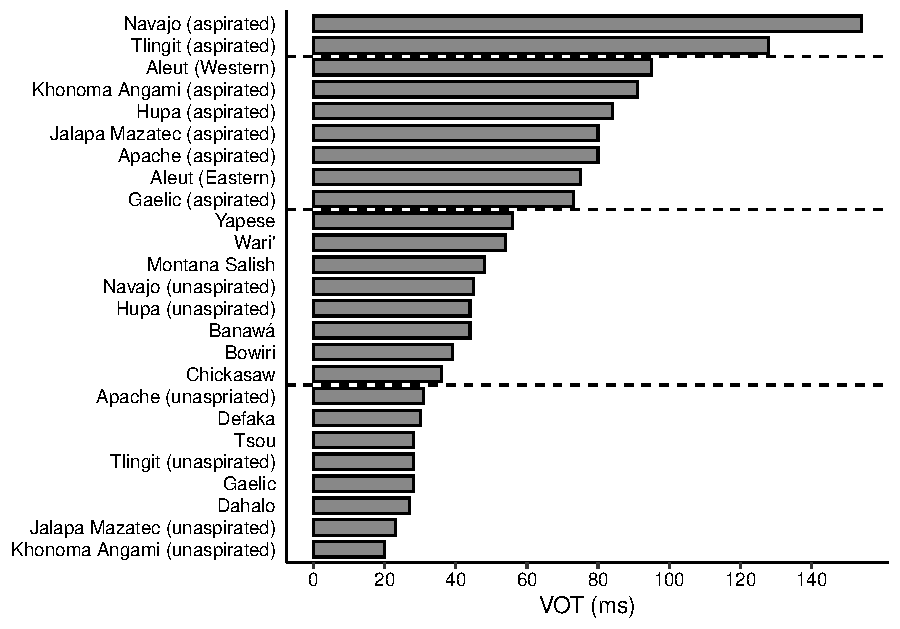
\includegraphics[width=\linewidth]{figures/ch2/real_vot.pdf}
\caption[Mean VOT values for velar stops from eighteen languages in the study of \cite{ChoLadefoged1999}]{Mean VOT values for velar stops from eighteen languages in the study of \cite{ChoLadefoged1999}. Dashed lines indicate the category boundaries assumed by the authors.}
\label{fig:cho_ladefoged_1999}
\end{center}
\end{figure}

To illustrate this point, if language drew on a fixed set of phonetic categories, the picture obtained by \cite{ChoLadefoged1999} should look more like the simulated data shown in Figure \ref{fig:simulated_vot}. Compared to this figure, the original picture resembles a continuous increase of VOT lacking clear jumps between the putative categories. Although this remains pure speculation, it is in line with \citet[42]{Ladd2014} who concludes that ``any apparent discontinuities in the gradual increase from one end of the VOT scale to the other would disappear" when more data were added to the picture of Cho and Ladefoged.

\begin{figure}[h]
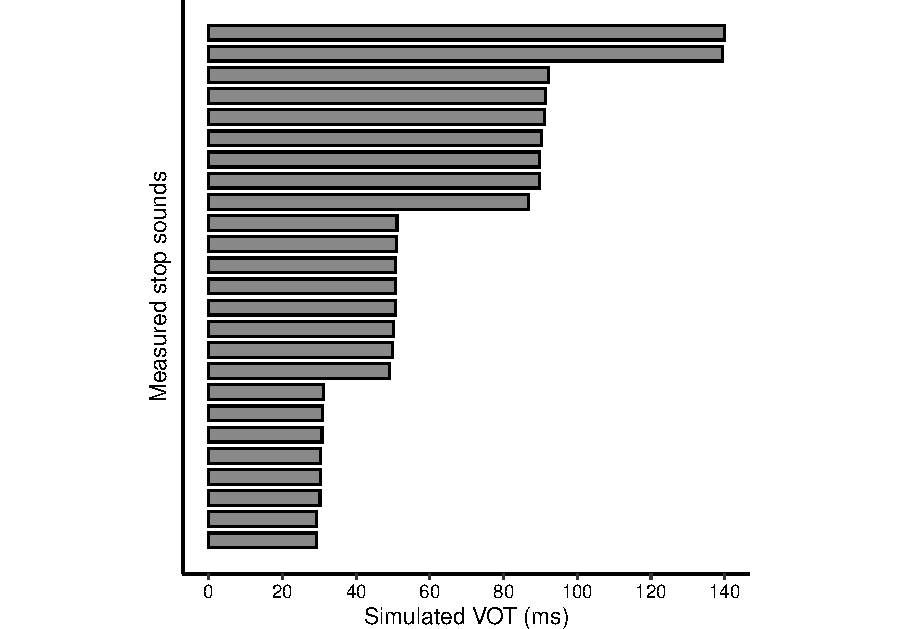
\includegraphics[width=\linewidth]{figures/ch2/simulated_vot.pdf}
\caption{Simulated VOT values under the assumption of a universal set of phonetic categories.}
\label{fig:simulated_vot}
\end{figure}

The idea of a universal set of phonetic categories is an integral part of a \emph{modular} view of phonetics and phonology. As mentioned above, the phoneme was seen as a psychological unit and supposed a division of the abstract representation in the mind and the physical realisation. In this way, phonetics and phonology are conceptualised as two modules from a cognitive perspective. More recent views that dispense with the phoneme and instead assume other representations like feature bundles adhere to a perspective in which modularity plays an important role.

In this perspective of modularity, phonological entities are stored and processed in one module and then passed on to a separate phonetic module to prepare and realise the implementation. Thus, phonetics and phonology are not only separated as scientific disciplines but also viewed as two disparate cognitive domains. Importantly, the separation into clear-cut cognitive modules necessitates translations from symbolic representations to continuous properties \citep{Ohala1990,GafosBenus2006} at the \emph{interface between phonetics and phonology} \citep{Keating1988} -- a term extensively discussed in the last decades. Because the domains are encapsulated and administer their own representations and carry out their own computations before passing the result to the next module, the receiving module cannot access the history of steps that lead to this particular representation. As  \citet[102]{Pierrehumbert2002} notes, the mainstream view of phonetics, phonology and their interface is architectured as a \emph{feed-forward} system ``because no arrows go backwards, from articulatory plans to phonological encoding".

\section{Gradience}
In the above outlined perspectives of phonology, its representations must only entail those features of sounds that cause differences in terms of lexical meaning. The continuous aspects of speech live only on the level of phonetic representations and come into being mainly as a consequence of universal characteristics of articulation, acoustics and audition. The phonological representations are discrete symbols that can be changed by applying discrete rules. An example for such a rule is the assimilation rule given in \ref{eq:assimilation_rule} as taken from \citet[262]{Nolan1992}. In this example, a unit characterised by the features [+coronal], [+anterior], and [$-$continuant] inherits the values of these particular features from the following unit. If this rule is applied to the sequence /leɪt kɔːlz/ (\emph{late calls}), the result would be [leɪk kɔːlz]. 

\begin{equation}
\begin{bmatrix} 
+\text{coronal}\\
+\text{anterior}\\
-\text{continuant}
\end{bmatrix} 
\rightarrow
\begin{bmatrix} 
\alpha \,\, \text{coronal}\\
\beta \,\, \text{anterior}\\
\gamma \,\, \text{continuant}
\end{bmatrix}
/\underline{\hspace{1cm}}
\begin{bmatrix} 
\alpha \,\, \text{coronal}\\
\beta \,\, \text{anterior}\\
\gamma \,\, \text{continuant}
\end{bmatrix}
\label{eq:assimilation_rule}
\end{equation}

Note how the /t/ turned into a [k] – one discrete entity was transformed into another discrete entity. \cite{Nolan1992} demonstrates, using electropalatography (EPG), that the process of assimilation is in fact a gradient process. This means that there are instances of /t/ for which it is possible to find the residual of an alveolar closure during the phase of the plosive. In some instances, there is no complete alveolar closure, but the tongue still has contact to the front parts of the gum. In other instances, the assimilation is complete and the contact is only velar. In these instances, the contacts are comparable to a /k k/ sequence as in /meɪk kɔːlz/ (\emph{make calls}). In addition to showing that assimilation is a gradient process rather than a discrete process in speech production, Nolan also provides evidence that listeners are able to use this gradient information in perception.

A framework that is able to capture gradient phenomena like this is \emph{Articulatory phonology} \citep{BrowmanGoldstein1986,BrowmanGoldstein1992}. In Articulatory phonology, speech sounds are not represented as symbolic units. Instead, the primitives of phonology are gestures. Patterns of speech sounds come into existence through the orchestration of multiple gestures in \emph{gestural scores}. These scores build higher forms, like syllables and words. Crucially, a gesture is viewed as a continuous dynamical system. This makes it possible to describe fine-grained differences in the spatial and temporal manifestations. Assimilation of a /t/ towards a /k/, like in the study of Nolan discussed above, is ascribed to an overlap of the tongue tip gesture for the alveolar closure and the tongue back gesture for the velar closure. The overlap of the two gestures can take any value on a continuous scale from no overlap to complete overlap. In this view, the timing relation of the two gestures is gradient and so is the phenomenon of assimilation. To illustrate how assimilation is modelled in Articulatory phonology, Figure \ref{fig:score_late_calls} shows gestural scores for two instances of \emph{late calls}.\footnote{The scores shown here might not provide a full detailed account of the gestural activations for this phrase, as for example the /l/ in English in word-medial positions is often described as ``dark". Therefore, /l/ in English may be better described by a tongue tip and a tongue back gesture that vary in the degree of overlap.}

A gestural score is a tabular visualisation of the gestural activations during the production of a word or phrase. The vertical axis shows the \emph{tract variables} that correspond to the recruitment of the articulators. In the cases shown here, tongue tip (TT), tongue body (TB) and glottis (GLO) are displayed. There are many more tract variables available in the Articulatory phonology modelling approach, for an overview see \cite{BrowmanGoldstein1992} and \cite{Mücke2018}, as well as the next chapter. The horizontal axis of the gestural score displays \emph{time} such that if an interval starts to the right of another interval, it is said to start later. The boxes give the description of the \emph{location} and \emph{degree of constriction} in a tract variable. The constriction locations used in the score in Figure \ref{fig:score_late_calls} are alveolar (alv), palatal, velar and uvular. The constriction degrees used in the scores comprise two types of closure: clo, denoting a full closure, and clo*, denoting a partial closure with a lateral opening. In addition, critical (crit) stands for a very narrow constriction resulting in friction noise. Finally, the degrees of constriction for the vowels used here are narrow and mid. For the glottis, wide simply indicates that the glottis is open for voiceless, it is closed for voiced otherwise.

\begin{figure}[h]
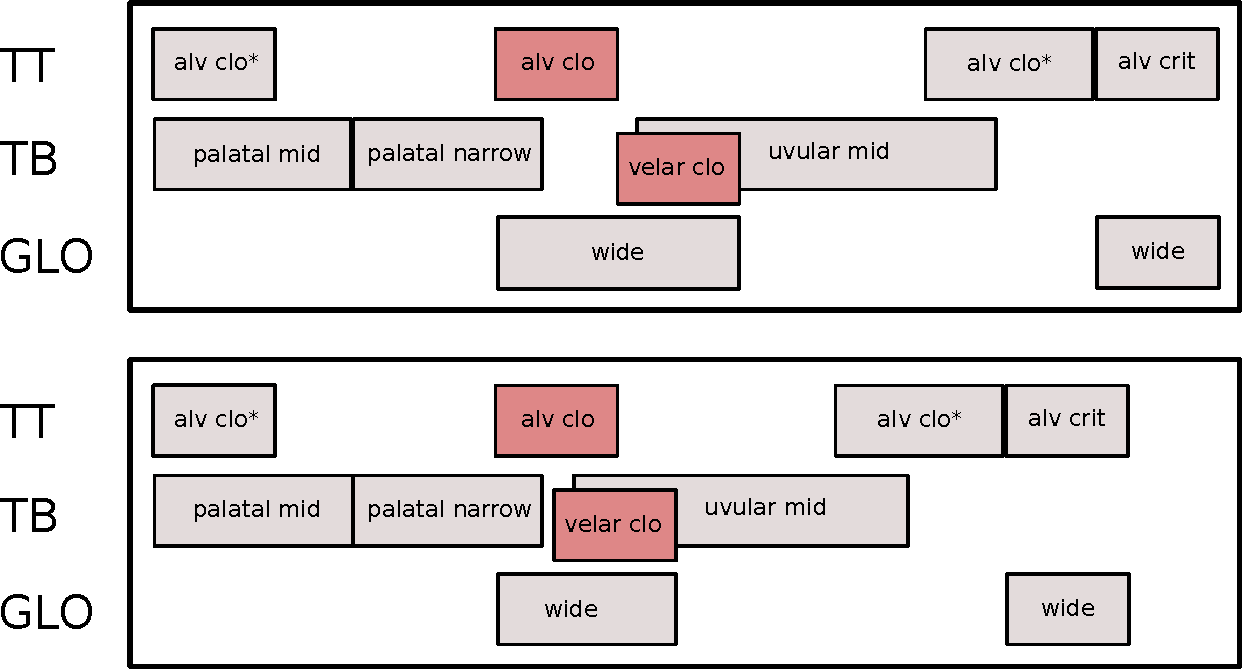
\includegraphics[width=\linewidth]{figures/ch2/late_calls.pdf}
\caption[Gestural scores of the utterance \emph{late calls}.]{Gestural scores of the utterance \emph{late calls} with no overlap of the two stop sounds (top) and high degree of overlap of the two stop sounds (bottom).}
\label{fig:score_late_calls}
\end{figure}

The example shows how the gestural organisation of Articulatory phonology models the gradience of a process like assimilation as continuous variation in the overlap of gestures. In the score at the top of Figure \ref{fig:score_late_calls}, there is no overlap between the alveolar closure gesture of the tongue tip (alv clo in the TT row) and the velar closure gesture of the tongue body (velar clo in the TB row). This score corresponds to a rather careful, clear rendition of \emph{late calls} that results in a clear differentiation of the velar and the alveolar stop. In the score at the bottom of the figure, the two gestures overlap to a large degree. In the acoustic signal corresponding to this score, the two stop sounds would not be differentiated well and hence assimilation would be recorded in a symbolic transcription. However, there is no manipulation or transformation of the set of phonological units involved here as in the rule of \ref{eq:assimilation_rule} where one symbolic representation was replaced by another. The framework models the process as a gradient change in a continuous phonological representation. Although the boxes and labels (e.g. mid vs. wide) in the gestural score make the modelling approach appear discrete, one has to bear in mind that the boxes and labels are just ``shortcuts". A gesture is defined as a continuous dynamical system \citep{BrowmanGoldstein1992,Hawkins1992}, constriction place and degree can vary continuously in this system. In consequence, a label like ``mid" stands for a scalar value on a continuous scale of constriction degree and not for a discrete symbol from a finite set.

The case of assimilation as described above is an example of \emph{gradience} in speech -- a concept that has gained growing attention in recent research in phonetics and phonology \citep{Cohn2006}. Since it is used to denote similar but different phenomena, the term gradience has to be differentiated here. \cite{Ladd2014} referring to \cite{Bolinger1961} distinguishes \emph{physical} from \emph{statistical} gradience. While physical gradience refers to detailed variation on a continuous scale, statistical gradience denotes variation in the statistical patterns of occurrence of an event that can be described as categorical. This differentiation will be referred to in the further course of this work. However, to avoid confusion with other uses of gradience, I will adopt a different terminology. Many scholars use the word gradience to exclusively describe what Ladd calls physical gradience, not statistical gradience. Hence, I will adopt the term \emph{variation} instead. Because statistical gradience or variation refers to the occurrence of categorical events or entities, the term \emph{categorical variation} will be used. Further, I will use the term \emph{continuous variation} to refer to what \cite{Ladd2014} calls physical gradience. 

Various theoretical frameworks have dealt with the development of an accurate description of variation. Articulatory phonology, as demonstrated above, provides a means to account for continuous variation as in the case of assimilation. Of course, using the ends of the continuum, it is also suited to describe categorical variation (e.g. no overlap vs. complete overlap). But most theories have focussed mainly on a categorical description of variable patterns in speech sounds. In turning to patterns of language usage, scholars in the variationist tradition of sociolinguistics decades ago acknowledged that multiple forms of a word may coexist. As a consequence, the rule-based framework endorsed by generative phonology was extended to entail variable rules \citep{Labov1969,CedergrenSankoff1974,Anttila2007}. A variable rule is applied optionally with a specific quantity that denotes how often the rule will be applied. Such a rule may be written in the form X $\rightarrow$ (Y) / A\_B with the parentheses indicating that the outcome of the rule is not generated in all cases (``X optionally turns to Y in the context between A and B").

Other modelling approaches that are able to describe patterns of categorical variation are stochastic extensions of \emph{Optimality Theory} (\citealp{PrinceSmolensky2004}; henceforth: OT). OT is a theoretical framework that works with symbolic representations but without rules. Instead, it uses ranked \emph{constraints} to evaluate the ``winner" from a set of possible \emph{output form} candidates for a given \emph{input form} \citep{Gussenhoven2004}. The winning output form is said to optimally satisfy the constraints and is delivered to phonetic implementation. The tableau in \ref{eq:ot_example} gives a simplified example for computation of the plural form of the English word \emph{kiss} from \cite{GussenhovenJacobs2011}. It uses the constraint \textsc{*SibSib} that is violated if the word contains two adjacent sibilants, the constraint \textsc{Dep-IO} that is violated if a segment not present in the input form is inserted, and the constraint *$\alpha$\textsc{voice}-$\alpha$\textsc{voice} that is violated if two adjacent sibilants do not share the same quality for the voicing feature (e.g. voiceless may not be followed by voiced). The constraints are ranked from left to right: \textsc{*SibSib} outranks \textsc{Dep-IO}, \textsc{Dep-IO} outranks *$\alpha$\textsc{voice}-$\alpha$\textsc{voice}. The symbol * denotes one violation of a constraint for the candidate in that row. The symbol ! indicates whether this violation is ``fatal" which means that this violation leads to the ``defeat" of this candidate. In the example in \ref{eq:ot_example}, candidate b is the only candidate that does not violate the constraint of the highest rank, \textsc{*SibSib}, and thus is the optimal form, marked with the symbol ☞. Of the two violations for candidate a, the violation of \textsc{*SibSib} is fatal because it already renders it a loser of the competition regardless of its violation of *$\alpha$\textsc{voice}-$\alpha$\textsc{voice}.
	
\begin{equation}
\begin{tabular}{|r|c|c|c|}
\hline
/kɪsz/ & \textsc{*SibSib} & \textsc{Dep-IO} & *$\alpha$\textsc{voice}-$\alpha$\textsc{voice} \\
\hline
a. kɪsz &  *! &  & *\\
\hline
☞  b. kɪsɪz &  & * & \\
\hline
c. kɪzz & *! & & \\
\hline
d.  kɪss & *! & & \\
\hline
\end{tabular}
\label{eq:ot_example}
\end{equation}

As can be seen in this simple example, a basic OT approach determines a single optimal form – and the same optimal form will be evaluated by the grammar every time unless the constraint ranking is changed. To implement categorical variation, a probabilistic mapping of input and output form, this account has to be extended. To illustrate the process, one case that will be treated more in-depth here is the probabilistic choice of suffixes in Hungarian \emph{vowel harmony} \citep{HayesLonde2006}. Vowel harmony has been described as a phenomenon in which the vowels within a word agree with regard to some phonetic property, like the place feature [±back] \citep{GafosBenus2006}. In Hungarian, for many stems, the quality  [±back] of the stem vowel determines the choice of the suffix such that the suffix agrees with the stem in its [±back] property. For example, the stem \emph{ablak} /ɔblɔk/ (`window') in which the last vowel is [+back] takes the suffix \emph{nak} /nɔk/ with a back vowel while the stem \emph{üst} /yʃt/ (`cauldron') with a front vowel takes the suffix \emph{nek} /nɛk/ with a front vowel \citep[62]{HayesLonde2006}. In addition, front unrounded vowels function as \emph{transparent or neutral vowels} \citep{HayesLonde2006}. These vowels can occur between the vowel triggering the vowel harmony and the target of the vowel harmony, e.g. the suffix vowels in the examples above, but do not affect the process of vowel harmony – even if their quality of the feature [±back] is opposing to the triggering vowel. For instance, the stem \emph{kávé} /kaːveː/ (`coffee') takes the suffix \emph{nak} /nɔk/ – the back vowel of the stem determines the vowel of the suffix regardless of the intervening unrounded front vowel. 

Interestingly, stems with a back vowel and one or two transparent vowels have been observed to be able to take back and front suffixes, with statistical preferences for one or the other. For instance, \citet{HayesLonde2006} observed that the stem /aːɲiveːl/ occurs with the suffix \emph{nek} /nɛk/ in 83.6\% of cases and with the suffix \emph{nak} /nɔk/ in the remaining 16.4\% of cases. The authors use stochastic OT \citep{Boersma1997,BoersmaHayes2001} to model this probabilistic suffix alternation. To give a full account is beyond the scope of this chapter. The following description is restricted to a short overview to exemplify how stochastic OT can account for categorical variation. The constraint rankings are not strict in this approach, rather the constraints are assigned ranking strength probabilities. The tableau in \ref{eq:stochastic_ot_table} uses three constraints: \textsc{Local[NN]} which is violated when a stem with two neutral vowels is followed by a back vowel, \textsc{Local}[e:] which is violated when the closest vowel following [e:] is a [+back] vowel, and \textsc{Distal[B]} which is violated when a [+back] vowel is followed by a [$-$back] vowel somewhere in the word.\footnote{This is not the complete set of constraints used by \citet{HayesLonde2006} to model the data, it represents a minimal example to illustrate the point of probabilistic constraint rankings.} The fact that they are not ranked strictly (or statically) as in the previous example is expressed by the dashed separation lines between the columns. The ranking strengths of the constraints are given by the probability density functions shown in Figure \ref{fig:probs_stoch_ot}. \textsc{Local[NN]} has a mean ranking strength of 101.802, \textsc{Local}[e:] has a mean ranking strength of 100.894, \textsc{Distal[B]} has a mean ranking strength 100.000. The standard deviation is 2 in all cases. From these ranking strength distributions, the probability for a given output form can be calculated. Candidate a in tableau \ref{eq:stochastic_ot_table} from \citet[81]{HayesLonde2006} violates \textsc{Distal[B]} three times, candidate b violates the other two constraints but \textsc{Distal[B]} only twice. For candidate b to win, the constraint \textsc{Distal[B]} has to be outranked by both \textsc{Local[NN]} and \textsc{Local}[e:]. The question is: If one ranking strength sample is taken from each of the three distributions presented in Figure \ref{fig:probs_stoch_ot}, how often will the two samples for \textsc{Local[NN]} and \textsc{Local}[e:] both be smaller than that for \textsc{Distal[B]}? The answer is: In 16.4\% of all cases. In all other cases, candidate a will win. The probabilities are given in the first column, to the left of the candidates.

\begin{equation}
\begin{tabular}{|r|c:c:c|}
\hline
/aːɲiveːl-nAk/ 		& 	\textsc{Local[NN]} & 	\textsc{Local}[e:] &		\textsc{Distal[B]} \\
\hline
0.836 ☞ a. aːɲiveːl-nɛk & 			         & 			       &		***(!) \\
\hline
0.164 ☞ b. aːɲiveːl-nɔk 	&         *(!)		         &	*(!)                       &       	 **\\\hline
\end{tabular}
\label{eq:stochastic_ot_table}
\end{equation}

\begin{figure}[h]
\begin{center}
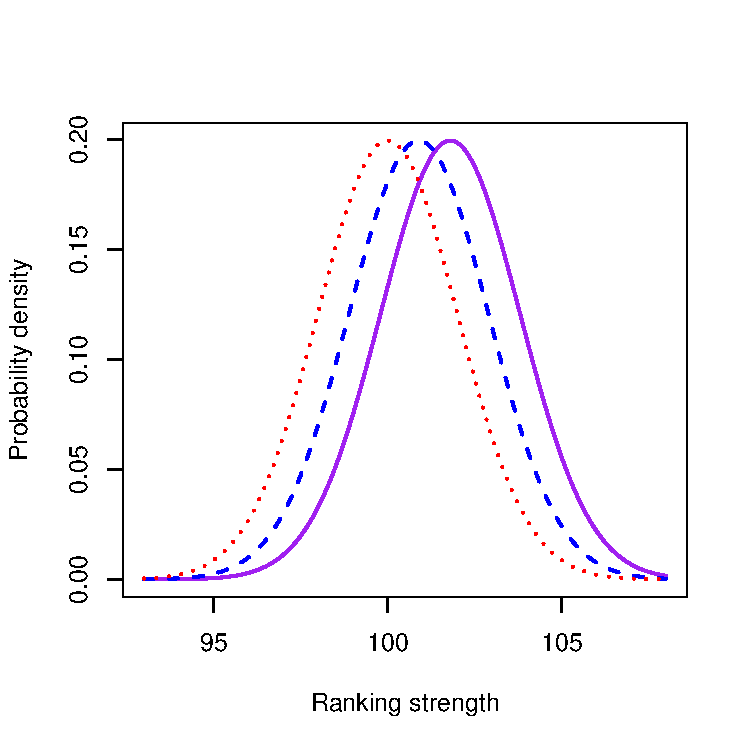
\includegraphics[width=9cm]{figures/ch2/stochastic_ot.pdf}
\caption[Ranking strength probabilities for the constraints of \citet{HayesLonde2006}.]{Ranking strength probabilities for the constraints based on footnote 15 of \citet{HayesLonde2006}. \textsc{Local[NN]} (purple, solid line), \textsc{Local}[e:] (blue, dashed line), \textsc{Distal[B]} (red, dotted line).}
\label{fig:probs_stoch_ot}
\end{center}
\end{figure}

As becomes clear from this example, stochastic OT is able to cope with statistically gradient patterns, or categorical variation, i.e. the statistical preference for one or another category. Continuous variation is not captured by this framework. In the next chapter, a dynamical systems approach to the problem of the probabilistic suffix choice in Hungarian will be outlined that focusses on continuous sub-symbolic variation \citep{GafosBenus2006}. This model builds on articulatory details and shows how continuous variation may contribute to categorical variation. 

As outlined in the introduction to this book (Chapter \ref{chapter_intro}), it is one of the aims of the present work to show that categorical and continuous variation often go hand in hand. This view is in line with \citet[88]{Ladd2014} who notes that ``[i]n many situations, of course, the two types of variation are likely to interact and reinforce one another." Motivated by the fact that categorical and continuous phenomena in speech often show a high degree of parallelism, \citet{Flemming2001} presents a model rooted in OT that combines continuous and categorical aspects and intends to reconcile phonetic and phonological representations in a formal approach. The main idea revolves around a trade-off of constraints rather than a categorical ranking of constraints. This trade-off can be determined by expressing the violation of each constraint as a scalar quantity. As a result, each possible candidate of the optimalisation process acquires a cost and the candidate with the lowest cost is selected as the optimal form. This approach will be outlined here in more detail using the example of assimilation of a back vowel to a coronal consonant.

It has been observed that in some languages the contrast between front and back rounded vowels is neutralised in the position between coronal consonants. For example, in Cantonese Chinese the forms /kʰyt/ (`decide') and /kʰut/ (`bracket') exist, as well as /tʰyt/ (`to take off'). There is, however, no form */tʰut/ \citep{Flemming2001}. This phenomenon has been described as a case of categorical assimilation, i.e. as the outcome of a phonological computation in which the  [+back] specification of the vowel is changed to [+front]. In other languages, a parallel process, the co-articulatory fronting of back vowels in the context of coronal consonants has been described as purely phonetic (and as such continuous). In English, for example, /u/ is produced more fronted in \emph{toot} /tut/ compared to \emph{coo} /ku/. 

The modelling idea of \citet{Flemming2001} involves the formulation of the following constraints based on a quantification of the second formant (F2) of both the consonants and the vowel. The constraint \textsc{Ident(C)} requires the target F2 of a consonant to be maintained. Its violation cost is the weighted squared difference between the realised F2 of the consonant and the target F2 of the consonant: $weight_c \cdot (F2(C) - L)^2$, where $F2(C)$ is the realised F2 of the consonant and $L$ is the target F2 of the consonant.

The constraint \textsc{MinimiseEffort} requires that the speaker reduces articulatory effort. It tries to keep changes in F2 from C to V as small as possible. Its violation cost is the squared difference between the realised F2 of the consonant and the realised F2 of the vowel: $weight_e \cdot (F2(C) - F2(V))^2$, where $F2(C)$ is the realised F2 of the consonant and $F2(V)$ is the realised F2 of the vowel.

The constraint \textsc{MinDist  = Δ} requires that the distance between the F2 of the vowel /u/ and its nearest neighbour /y/ is above a certain threshold. Its violation cost is the weighted difference between the distance of /u/ and /y/ in terms of F2 and the threshold: $weight_v \cdot (|F2(y) - F2(u)| - \Delta)^2$, where $F2(y)$ is the F2 of the vowel /y/, $F2(u)$ is the F2 of the vowel /u/, and Δ is the minimum distance between the two, the threshold. This constraint only applies if the contrast is maintained. Its violation cost is not calculated if the contrast is neutralised, i.e. the assimilation is categorical.

In addition, the model uses the quantity \textsc{MaximiseContrast}. This value represents the benefit of preserving a contrast. While the other three constraints acquire positive costs as they are violated, \textsc{MaximiseContrast} is subtracted as a negative cost.

The candidates of the optimisation process are inventories of contrasting syllables. First, the total violation cost for a candidate is calculated as the sum of all single weighted violation costs for the constraints. Second, the benefit of maintaining the contrast, \textsc{MaximiseContrast}, is subtracted. After these steps, the inventory with the lowest cost is selected as optimal. Thus, if the benefit of maintaining the contrast is exceeded by the costs obtained by the distinctiveness and effort constraints (\textsc{Ident(C)}, \textsc{MinDist = Δ}, and \textsc{MinimiseEffort}) in the realisation of /tut/, it is optimal to neutralise the contrast between /u/ and /y/. The consequence is \emph{categorical assimilation}. On the contrary, if the combined costs for the violation of the constraints \textsc{Ident(C)}, \textsc{MinDist = Δ}, and \textsc{MinimiseEffort} do not exceed \textsc{MaximiseContrast}, neutralisation in the form of categorical assimilation is not optimal. However, as a trade-off between \textsc{Ident(C)} and \textsc{MinimiseEffort}, \emph{co-articulatory assimilation} with varying degrees follows. In this model, the difference between languages can be modelled by using the same sets of constraints and modulating the value for \textsc{MaximiseContrast} as well as the weights for the violation costs of the constraints as scalar values. Depending on how the weights are set, the costs for distinctiveness and effort might exceed the benefit of maintaining a contrast or not \citep{Flemming2001}.

Similar to Articulatory phonology, Flemming's approach models degrees of assimilation in the same formal system and does not distinguish between categorical, phonological and continuous, phonetic processes. In Articulatory phonology, assimilation is a fundamentally continuous process as the organisation of gestural activation varies on the continuous dimension of time -- affecting the temporal and spatial properties of the phonetic outcome. Categorical behaviour can be found at the ends of the continuum. In Flemming's model, the trade-off between the benefit of contrast preservation and the costs connected to effort and distinctiveness of sound pattern explains the outcome as categorical or continuous assimilation. In both modelling frameworks, categorical variation on the ``macro-level" is seen as the result of the interaction of variation on continuous dimensions on the ``micro-level".

\section{Tiny differences, rich memory}
Another famous example that poses a problem for the modular view of phonetics and phonology is the phenomenon known as \emph{incomplete neutralisation}. It describes the finding that the neutralisation of the voicing contrast of syllable-final obstruents present in some languages as the result of \emph{final devoicing} is indeed incomplete. Final devoicing or \emph{Auslautverhärtung} is a classic textbook example showing that voiced obstruents at the end of syllables turn into voiceless obstruents in German. Thus, the contrast between voiced and voiceless is said to be \emph{neutralised} in this context. Similar phenomena have been observed in other languages as well \citep{Bloomfield1933}. In a modular, symbolic account of the case, the voiced obstruent is transformed into a voiceless obstruent at the end of syllables by virtue of a phonological rule like the one given in \ref{eq:final-devoicing} (where \$ stands for the end of a syllable). This rule is suited to turn a structure like /ʁad/ into [ʁatʰ] and thus makes the difference between the phonetic outputs of the words \emph{Rad} (`wheel') and \emph{Rat} (`advice') disappear completely.

\begin{equation}
\text{[+voiced]} 
\rightarrow 
\text{[$-$voiced]}
/\underline{\hspace{1cm}}\$
\label{eq:final-devoicing}
\end{equation}

Contrary to the prediction of this rule, a considerable number of studies found that the acoustic signals of words like \emph{Rat} and \emph{Rad} are different \citep{DinnsenGarciaZamor1971, PortODell1985, CharlesLuce1985, PortCrawford1989, ErnestusBaayen2006, Roettgeretal2014}. In general, the voicing contrast can be encoded by different phonetic cues like glottal pulsing in the closure of the stop, closure duration, voice onset time, but also duration of the preceding vowel \citep{Lisker1986}. Studies on the incompleteness of the voicing contrast demonstrated that the differences between the acoustic signals regarding these parameters go in the direction of a voicing contrast in inter-vocalic position as in \emph{Räder} vs. \emph{Räte}, although the differences are much smaller. Recently, \cite{RoettgerBaerHenney2019} added convincing empirical evidence for the robustness of the incompleteness of German final devoicing using a large, diverse data set.

An approach based on discrete symbolic representations and rules, like the one outlined in \ref{eq:final-devoicing}, is clearly not able to account for the continuous, subtle variation reported by the studies above. The question arises how the difference between the two obstruents can be best captured in a model of phonetics and phonology. An early proposal by \cite{PortODell1985} is to employ \emph{phonetic implementation rules}. While phonetic implementation rules were already implicitly assumed by earlier models \citep[like][]{ChomskyHalle1968, JacobsonFantHalle1952}, they were not considered linguistic in a strict sense, i.e. not part of langue. \cite{PortODell1985} extend the classic model of separated phonetics and phonology by considering language-specific phonetic implementation rules that belong to the speaker's knowledge of the language. To account for the incompleteness of final devoicing in German, the authors use a rule that phonetically implements the syllable. It is the duty of this rule to devoice a voiced obstruent at the end of syllables. Thus, the voiced obstruent retains its phonological specification [+voiced] during the stage of phonological derivation. Only later, at the stage of phonetic implementation, a gesture is activated that resembles the one found with sounds that possess the phonological quality [$-$voiced]. 

While the inclusion of a phonetic rule that is in fact part of the language ``makes the relationship between phonetics and phonology closer by permitting the phonetic implementation system to directly execute the macrostructures in the phonology” \citep[468--469]{PortODell1985}, it strictly adheres to the modular view of phonetics and phonology. In fact, it emphasises the separation between the two modules despite making them more similar. In a footnote, \cite{PortODell1985} entertain the interesting idea that \emph{rules} might not be the right devices in general to account for the cognitive underpinnings of language and speech. In the next chapter (Chapter \ref{chapter_ds}), a dynamical model for the subtle differences observed in the syllable-final obstruents in German is introduced \citep{Gafos2006, GafosBenus2006}. This model does not assume rules or a separation of categorical and continuous aspects. As will become clear in this chapter, despite using a continuous formalism, the model is nevertheless able to explain the categorical nature of the [±voiced] feature.

Other accounts have modelled the phenomenon as an artefact of lexical co-activation, also known as \emph{phonetic paradigm uniformity}, without the need for the invention of a new kind of rules \citep[e.g.][]{ErnestusBaayen2006, GoldrickFolkRapp2010, KleberJohnHarrington2010, WinterRoettger2011, Roettgeretal2014, SeyfarthKlokGarellek2019}. The basic idea behind these approaches is that the mental lexicon stores a collection of rich auditory forms of words, like \emph{Rad}, \emph{Räder}, and \emph{Rades}, rather than abstract representations and rules to produce derived forms. During the activation of a word like \emph{Rad}, close lexical neighbours like \emph{Räder} and \emph{Rades} are co-activated. These co-activated forms enhance the probability that the final obstruent of \emph{Rad} is realised with phonetic characteristics slightly pushed in the direction of a voiced obstruent \citep{ErnestusBaayen2006, Roettgeretal2014}. 

These approaches are rooted in a framework known as \emph{exemplar theory}. Exemplar theory, originally proposed in psychology for the classification of multi-dimensional stimuli more generally \citep{Nosofsky1986, Hintzman1986}, has gained a lot of attention in phonetics and phonology. It postulates detailed, episodic memory of acoustic traces of words as the basis of speech production and perception \citep[among others]{Goldinger1996, Johnson1997, Pierrehumbert2001, Bybee2001, Pierrehumbert2016}. Exemplar theory is thus fundamentally different from rule-based or constraint-based theories of phonology which, as outlined above, assume abstract units to achieve ``maximally simple, redundancy-free representations" \citep[213]{GahlYu2006}. Exemplar theory postulates that the detailed experiences of language use shape the cognitive representation of speech sounds through memorisation of the particular signal (or at least parts of it). Every time a speaker hears a word -- be it spoken by another person or herself -- a new acoustic trace called \emph{exemplar} is stored in her memory near the location of the existing exemplars. During the perception and the production of speech sounds, clouds of stored exemplars are activated. In the case of categorisation, the incoming stimulus is compared against the rich inventory of exemplars. The stimulus will be categorised as belonging to the group of stored exemplars that are most similar. In the case of production, the stored clouds of exemplars serve as production targets. In both perception and production, newer exemplars have more influence since memory traces fade away over time \citep{Schweitzer2012}.

Exemplar models are able to account for experimental findings demonstrating the importance of fine-grained phonetic detail in both perception and production \citep{Pierrehumbert2016}. For example, \cite{Wright1979} as well as \cite{Jurafskyetal2002} showed that more frequent words are produced faster and more reduced compared to less frequent words. This finding also applies to words that are more predictable from the context \citep{Seyfarth2014, AylettTurk2004, Halletal2018}. From an exemplar-based perspective, articulatory effort can be seen in relation to the likelihood of activation. A lexical item with a large cloud of exemplars is activated more easily than a lexical item with a smaller cloud. As outlined above, each time a word is perceived, its acoustic trace is added to the existing exemplars. Hence, less articulatory effort is needed for the transmission of words that are heard very frequently since their exemplar clouds generally accumulate more traces. 

In addition to frequency, lexical access can also be facilitated by many other factors, like indexical information about the speaker producing the word: \cite{WalkerHay2011} showed that listeners were faster and more accurate in lexical decision for words that are more frequently heard in real life said by older speakers, like \emph{typist}, when these words are produced by an older voice in the experiment. Vice versa, words that are more frequently heard in real life from younger speakers, like \emph{checkout}, were more easily processed in the experiment when produced by a younger voice.

Exemplar theory emphasises the importance of phonetic detail for our understanding of speech and offers a completely different view on the relation between phonetics and phonology. While abstractionist frameworks like the rule-based or constraint-based models presented in this chapter view phonology as a reduced, abstract structure that is efficient in terms of memory consumption, exemplar theory posits that the speaker stores and uses large pools of real, experienced ``data". While abstractionist models operate on segment-sized units that in some sense adhere to the phonemic principle, exemplar theory uses larger chunks like words. Scholars in the abstractionist tradition have often highlighted that segment-based approaches are good at explaining the regularities in sound change throughout the whole phonological system, like \emph{chain shifts} described by Grimm's law \citep{Guy2014}. Exemplar theorists on their part have argued that sound changes may not necessarily be regular. While Middle English long /o/ in today's English turned into /u/ in words like \emph{root} and \emph{food}, it also developed into /ʊ/ in words like \emph{good} and \emph{book} or schwa as in \emph{flood} \citep{Guy2014}. However, pure exemplar approaches have difficulties dealing with regularities in sound change – even if these regularities might not complete \citep{Pierrehumbert2016}. Further critique towards purely ``data-driven" exemplar models includes evidence that in addition to \emph{token frequency} (accumulated traces of perceived words), \emph{type frequency} of a lexical unit plays a role for the productivity of this pattern \citep{HayPierrehumbertBeckman2004}. 

As a consequence, exemplar-based approaches have been extended to \emph{hybrid models} which argue that abstract phonological representations also play a role. One of these models is delivered by \cite{Pierrehumbert2002} positing that abstract generalisations and exemplar clouds can be associated with phonological units like phonemes, sequences of phonemes, or words \citep[see also][]{GermanCarlsonPierrehumbert2013}. The model makes a distinction between production and perception. In production, phonological units play a major role but exemplars bias the production goals of the abstract units. On the contrary, in perception, exemplars play the leading role. The related \emph{Polysp} model \citep{HawkinsSmith2001, Hawkins2003} emphasises that identification of meaning in communication ``takes place probabilistically, using all possible available information in parallel to flesh out linguistic structure at all levels" \citep[391]{Hawkins2003}. Following this model, a listener might analyse a given acoustic signal into abstract linguistic units and match the signal with exemplars \citep{Ernestus2011}. Notably, in \emph{Polysp}, exemplars can include non-acoustic memory like visual information. \citet[8]{Sumneretal2014} endorse a similar view stating that ``[l]isteners simultaneously extract linguistic and social information from speech". While hybrid approaches offer promising explanations and testable predictions, \cite{Ernestus2011} notes that a full computational implementation of these models is still in progress.

\section{Summary}
In this chapter, the relation of phonetics and phonology was explored. It was outlined that the 20th century, with the rise of the phonemic principle, introduced a rather sharp separation between continuous, physical phonetics and categorical, symbolic phonology -- a distinction that was weaved into the fundamentals of linguistics. Even models in the tradition of \citet{ChomskyHalle1968} that dispense with the concept of the phoneme in a strict sense maintain the split as an important assumption. The chapter reviewed some of the problems which challenge a clear-cut separation and highlighted that many scholars nowadays assign a significant role to fine phonetic detail in cognitive representations of sound patterns as well as storage in memory. In this context, it becomes increasingly important to investigate how theoretical approaches are able to deal with continuous and categorical variation in sound patterns and linguistic structure. Models rooted in the framework of dynamical systems offer promising solutions for reconciling the continuous and categorical aspects in one formal language. Since the focus of this book is on modelling approaches within this framework and what they have to offer for an understanding of the relation of categorical and continuous aspects of speech, the next chapter introduces the foundations of dynamical systems and reviews important applications.

  
%\chapter{Dynamical Systems}
\label{chapter_ds}

The previous chapter reviewed models of phonetics and phonology and highlighted the importance of the ability to capture both categorical as well as continuous aspects of speech. Many problems that arise in modelling the relation of these aspects are connected to the use of fundamentally different representations. While phonology is modelled as a system of discrete computations, phonetics is conceptualised as essentially continuous \citep{Gafos2006}. Hence, in a many wide-spread models, ``a mapping between a categorical symbolic representation and a quantitative physical signal" \citep[8]{Ladd2006} is necessary. In contrast to these translational approaches, dynamical systems offer an alternative by employing a single formal language to capture both categorical and continuous aspects of speech. The potential of dynamical systems can be attributed to the fact that categorical behaviour emerges from continuous changes of parameters in a continuous space of possible states.

The last decades have seen a growing body of research that has pointed out the dynamical nature of the mind \citep[e.g.][]{Kelso1995,vanGelderPort1995,Port2002,Spivey2007,Kelso2013}. In order to overcome limitations imposed by purely symbolic approaches, researchers from many disciplines have turned to the framework of dynamical systems describing a multitude of different cognitive processes. Dynamical models for action and perception in cognition, including language and speech, emphasise the idea that the mind ``travels" through a continuous, many-dimensional space towards stable states \citep[4]{Spivey2007}. This idea is in sharp contrast to the traditional conception of the mind working like a computer that manipulates and replaces symbolic representations \citep{Fodor1975, FodorPylyshyn1981, Harnad1990, NewellSimon1976}. In a continuous, dynamical conception of cognition, the mind smoothly passes through multiple states during the process of settling in one stable state, rather than abruptly exchanging one symbol for the other. This perspective aims to shed light on the unfolding of a cognitive process over time and the relative stability of what can be described as a category in relation to other categories \citep{Port2002, GafosBenus2006, Spivey2007}. 

The present chapter concentrates on the basic concepts of the mathematics of dynamical systems and their applications to the description of patterns in speech. It attempts to be as illustrative as possible and serves as a background for the modelling approach of the present book for readers who are not familiar with the topic. The chapter is accompanied by MATLAB scripts that run the simulations and produce the plots shown alongside the text. The code can be retrieved here: \href{https://osf.io/4g6s2/}{https://osf.io/4g6s2/}. Details about which scripts are used can be found at the end of each section.

\section{The fundamentals of dynamical systems}

Complex, dynamical systems are found in all aspects of the world. Importantly, in such systems, the patterns of behaviour of the system emerge from the interaction of the parts of the system \citep{Fuchs2013, deBoer2001}. This feature distinguishes them from other systems in which the behaviour is determined by a hierarchical structure, for instance structure that is built-in by design as in many engineered systems.  A striking example is the formation of a traveling wave, called \emph{la ola} or \emph{Mexican wave}, through a crowd of people in a stadium -- a phenomenon that has been scientifically studied by \citet{FarkasHelbingVicsek2002}. To form the wave, individuals successively stand up and raise their arms. Crucially, this collective, coherent behaviour can neither be triggered, killed, slowed down or speeded up by a single individual \citep{Fuchs2013}. It arises under certain conditions when a small, critical mass of people initiates the movement. For example, since the level of excitement has to cross a certain threshold, it does not arise when the home team is losing. If it starts, the wave can spread over many thousands of people through the local interaction of individuals: Active individuals activate near-by individuals to stand up and raise their arms. Thus, the global near-linear shape of the wave emerges as the result of an interaction of the single parts of the system over time \citep{FarkasHelbingVicsek2002}.

To understand dynamical systems and their application to describe phenomena in the speech, language and cognition sciences, it is useful to look at some of the basic concepts of dynamical systems. This section will concentrate on these basics without providing a full introduction to the topic. Interested readers are referred to \citet{Fuchs2013}, \citet{KaplanGlass1995} and \citet{Iskarous2017} among many other great fully-fledged introductions to dynamical systems.

\subsection{Order and chaos}

The aim of the theory of dynamical systems theory is to create compact mathematical descriptions of the behaviour of complex systems like the \emph{la ola}. In doing so, dynamical systems focus on how a system changes over time based on the state that the system is currently in. To get a general understanding, it is helpful to study the \emph{logistic map}, a system formulated to describe the development of populations that was made popular by biologist \citet{May1976} as a discretised version of the demographic model proposed by Belgian mathematician Verhulst in the mid 19th century. The logistic map is given in Equation \ref{eq:logistic_map}.

\begin{equation}
x_{t+1} = kx_t(1-x_t)
\label{eq:logistic_map}
\end{equation}

The formula defines how the state $x$ of the system at a time point $t+1$ is calculated. Crucially, this future value of the state variable $x$ depends on the current state at $t$. In addition, the system has a parameter $k$ that represents the \emph{growth rate}. For example, if $k = 0.7$ and $x_1 = 0.5$ at the present time point, the system will predict $x_2 = 0.7 \cdot 0.5 \cdot (1-0.5) = 0.175$ at the next time point. Figure \ref{fig:logistic_map} shows how the evolution of the system is continued over 19 additional time steps. The graph shows that the points gradually approach zero. In terms of a population model this means extinction of the population. As there is no member of the population left to reproduce, the system will stay in the state with the value zero forever. This state is called the \emph{attractor} of the system. Regardless of the state of the system in the beginning, the system will end up in this state.

\begin{figure}
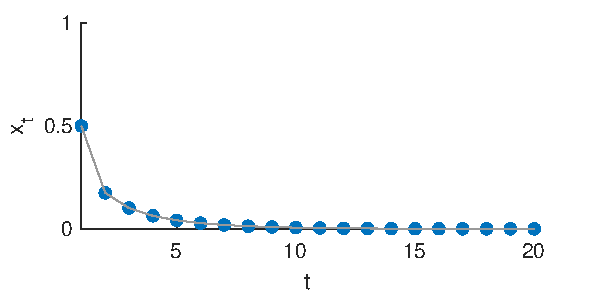
\includegraphics[width=8cm]{figures/ch3/logistic_map.pdf}
\caption{Example for the evolution of the logistic map with $k = 0.7$ and $x_1 = 0.5$.}
\label{fig:logistic_map}

\end{figure}

Depending on how the growth rate is chosen, the system can exhibit a variety of patterns. Figure \ref{fig:more_logistic_maps} gives examples for the logistic map with different values for the growth rate $k$. In all cases, $x_1$, the initial state, is $0.42$. In the case of $k = 1.2$ (top left), the system monotonically approaches one value. This type of attractor is called \emph{point attractor}, it is the same kind of attractor as the one in the illustration of Figure \ref{fig:logistic_map}. In the case of $k = 2.9$ (top right), the system also approaches one steady state, but while approaching the attractor, it alternates from one side to the other. When $k = 3.3$ (bottom left), the attractor of the system is not a steady state. Instead, the system oscillates between two values. This is type of attractor is called a \emph{limit cycle}. Another interesting case is $k = 4$ in which the system also oscillates but not in a periodic manner. This behaviour is called \emph{chaos} \citep{KaplanGlass1995}. When exhibiting chaotic behaviour, the system will never settle in a steady state or limit cycle but oscillate forever without repeating itself. 

\begin{figure}
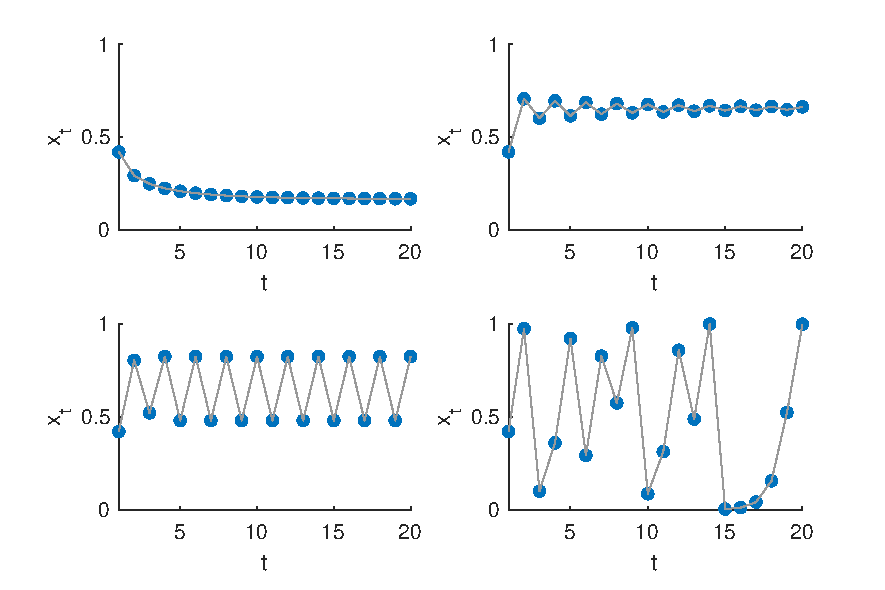
\includegraphics[width=\textwidth]{figures/ch3/more_logistic_maps.pdf}
\caption[Example for the evolution of the logistic map with different values for the growth parameter.]{Example for the evolution of the logistic map with different values for the growth parameter (top left: $k = 1.2$, top right: $k = 2.9$, bottom left: $k = 3.3$, bottom right: $k = 4$).}
\label{fig:more_logistic_maps}
\end{figure}

Figure \ref{fig:logistic_map_bifurcation} illustrates the possible patterns of the logistic map as the growth parameter is changed. The plot, also known as a \emph{bifurcation plot} \citep{Feigenbaum1978}, was created by running the logistic map for 2000 iterations for all growth parameter values between 1 and 4 with a step size of 0.01 (i.e. the simulation was first run with $k = 1$, then $k = 1.01$, then $k = 1.02$, and so on). The initial state is $0.42$ in all simulations. The axis for the parameter value is the x-axis. Of the 2000 iterations for each parameter value, the last 100 values are plotted on the y-axis as single tiny dots. For $k < 3$, all dots are plotted on top of each other because after a few iterations the system reached a steady state. As the parameter $k$ is increased, the system’s attractor is a limit cycle that oscillates between two values. The cycle frequency is then increased to 4, 8, 16 until the system eventually exhibits aperiodic behaviour as described above. There are, however, bands of growth parameter values in between for which the system moves back to periodic cycles (visible as white stripes in the higher regions on the x-axis) \citep{KaplanGlass1995, Spivey2007}. The behaviour of the system as $k$ is scaled beyond 3.5 can be observed in more detail in Figure \ref{fig:logistic_map_bifurcation_zoom}. This figure shows the same plot as Figure \ref{fig:logistic_map_bifurcation} with the x-axis zoomed in to the range of $k$ values from 3.5 to 4.

\begin{figure}
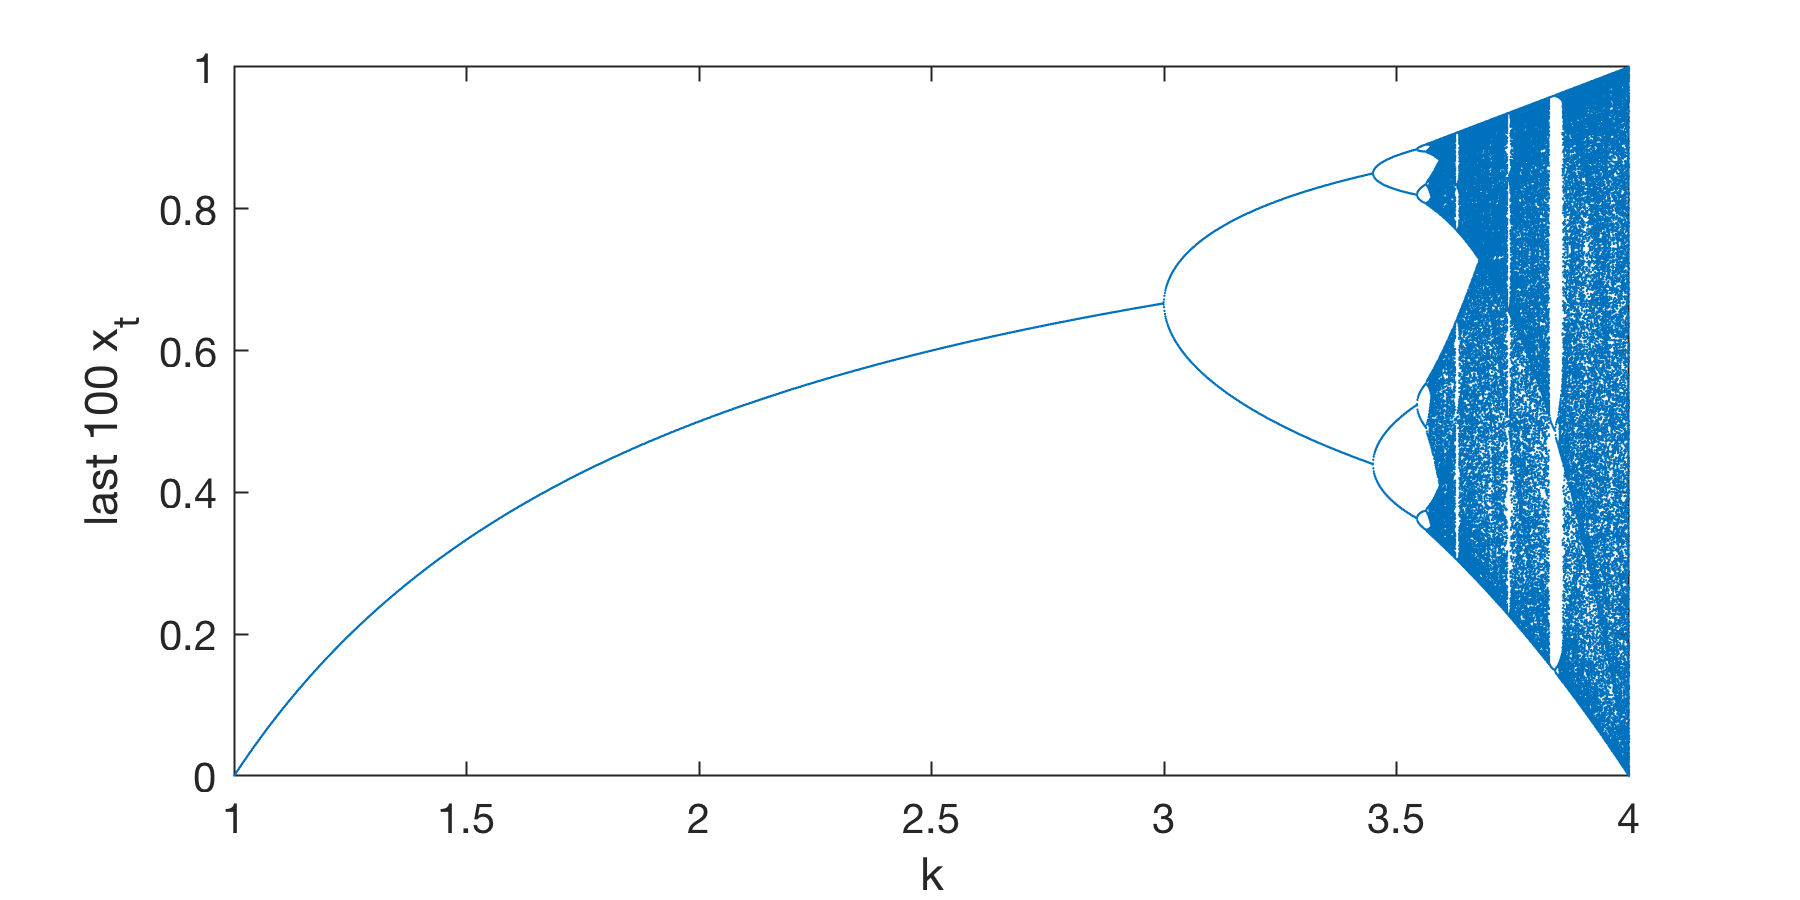
\includegraphics[width=\textwidth]{figures/ch3/logistic_map_bifurcation.png}
\caption{Bifurcation plot of the logistic map.}
\label{fig:logistic_map_bifurcation}
\end{figure}

\begin{figure}
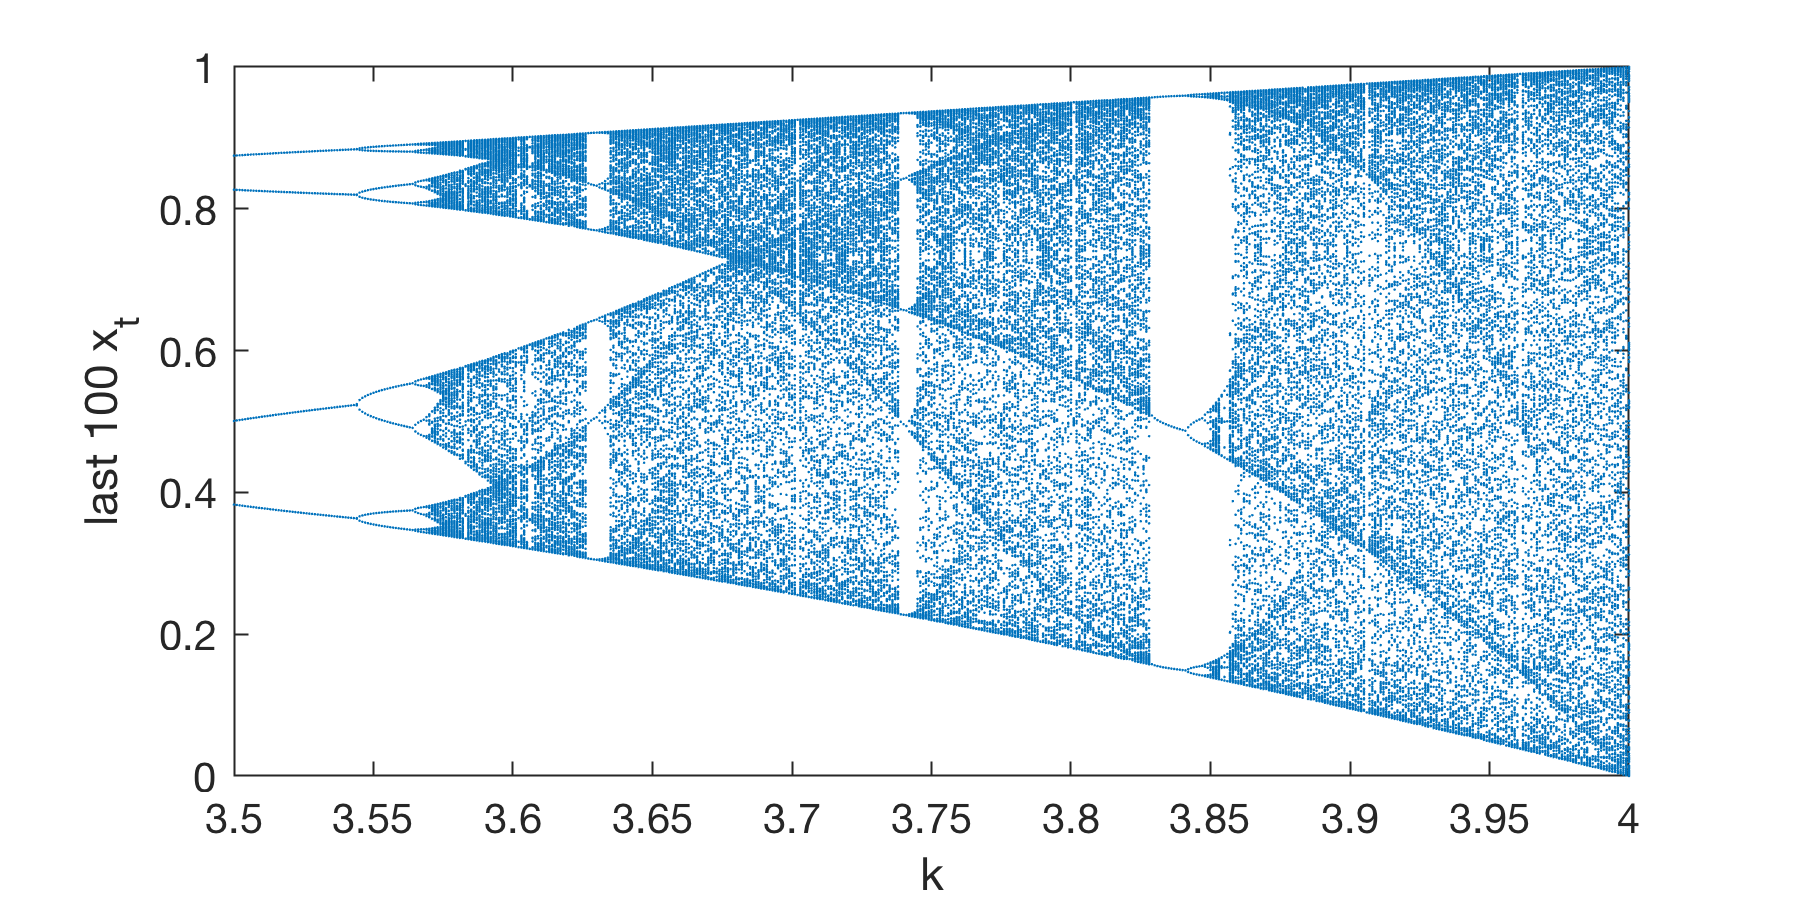
\includegraphics[width=\textwidth]{figures/ch3/logistic_map_bifurcation_zoom.png}
\caption{Bifurcation plot of the logistic map for values of $k \geq 3.5$.}
\label{fig:logistic_map_bifurcation_zoom}
\end{figure}

The examples presented around the logistic map demonstrate that an attractor can be a single value or a set of values. For the present work, point attractors will be most important. To change the behaviour of the system, the examples adjusted the growth parameter value $k$. A parameter like $k$ is called a \emph{control parameter} -- a very important concept for the understanding of dynamical systems. Control parameters can be thought of as the parameters that ``move the system through its repertoire of patterns and cause them to change" \citep[1538]{Kelso2013}. They often represent environmental conditions, like the growth parameter in the logistic map example, but are not restricted to this role \citep{Kelso2013}. 

An essential property of dynamical systems is that they often exhibit \emph{qualitative change} as the control parameter is scaled. This behaviour is referred to as \emph{bifurcation} -- a term used above already with regard to Figure \ref{fig:logistic_map_bifurcation} and \ref{fig:logistic_map_bifurcation_zoom}. As the name of the chart displayed in the two figures, bifurcation plot, already suggested, it shows how the logistic map undergoes bifurcation as the control parameter (the growth parameter) is increased. While the system starts with a point attractor, it changes into a pattern with a limit cycle as the control parameter passes a critical threshold. Subsequently, for other control parameter thresholds, the periods of the cycles change before the system turns to aperiodic behaviour. It then changes between aperiodic and periodic patterns for different ranges of control parameter values. All these transitions are qualitative changes, i.e. bifurcations, in the dynamical system.

\medskip\noindent \textit{Code used in this section: logistic\_map\_evolution.m, logistic\_map\_bifurcation.m}

\subsection{The use of differential equations in dynamical systems}
\label{sec:diff_equations}

In the logistic map, time progresses in discrete steps (or generations). When solving the equation, one considers the time points $t_1, t_2, t_3, ..., t_n$. In reality, of course, time is best characterised as continuous. A very common way to describe a dynamical system with reference to continuous time is by using \emph{differential equations}. The equation in \ref{eq:straight_line} gives a simple example for a differential equation. It uses a very common notation with a dot above the $x$ which denotes that the function is a derivate with respect to time, $\dot{x} = \frac{dx}{dt}$ \citep{Fuchs2013}. The basic idea in this system is very similar to the logistic map: We observe the behaviour of the state variable $x$. To learn about the change of the system at each state of $x$, the differential equation of the system is solved.

\begin{equation}
\dot{x} = kx
\label{eq:straight_line}
\end{equation}

To get an impression of what this simple system does, it is useful to start at some randomly chosen state and look at the evolution of the state variable $x$ over time. One way is to use a method known as the \emph{Euler method}, named after Swiss mathematician Leonhard Euler.\footnote{There are also other methods to solve differential equations, like the Runge-Kutta method. For some systems, like the one of Equation \ref{eq:straight_line}, it is also possible to give an exact analytical solution. For the exposition of systems considered in this work, subtle differences between the methods do not play a role.} Simply speaking, this method takes the change at the current state -- calculated by solving the differential equation of the system -- and adds it to the current state. Given that the state at some time point $t$ is known, the state at time point $t+h$ can be calculated easily as $x_t + hkx_t$ \citep{Fuchs2013} where $h$ denotes the size of the step that is taken in time (also expressed as $\Delta t$). As noted above, time is conceptualised as continuous in differential equations with regard to time, so using a discretising solution seems somehow paradoxical. However, it provides an easily implemented computation method for the solution of differential equations and the step size $h$ can be chosen very small to account for the fact that in continuous time the difference between $t$ and $t+1$ converges to zero. For the present work, the approximation of continuous time with sufficiently small time steps will be accepted as it will not disturb the results of the account. Figure \ref{fig:evolution_of_straight_line1} presents the evolution of the system of \ref{eq:straight_line} with a $k$ of $-0.5$ starting at the initial state $x = 0.42$. Similar to the example of \ref{fig:logistic_map}, this system approaches an attractor at zero.

\begin{figure}
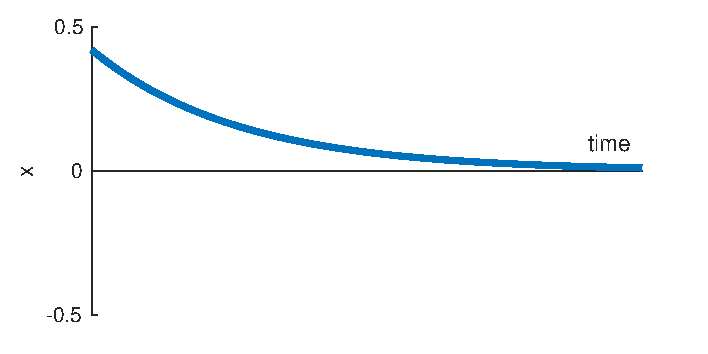
\includegraphics[width=9.5cm]{figures/ch3/evolution_of_straight_line1.pdf}
\caption{Evolution of the system given by the differential equation $\dot{x} = kx$ for $k = -0.5$.}
\label{fig:evolution_of_straight_line1}
\end{figure}

Figure \ref{fig:evolution_of_straight_line2} demonstrates the effect of scaling the control parameter. For all values of $k$, the system stays at zero if the initial state is zero (yellow lines). This is because the change in the system is given by $\dot{x} = kx$ and if $x$ is zero, the change will be zero as well. For all other initial values, the following pattern can be observed: $k$ values smaller than zero make the system approach the attractor at zero. For k values greater than zero, the system does not converge to any attractor. With $k = 0$ the system does not change at all but stays in its initial state. 

\begin{figure}
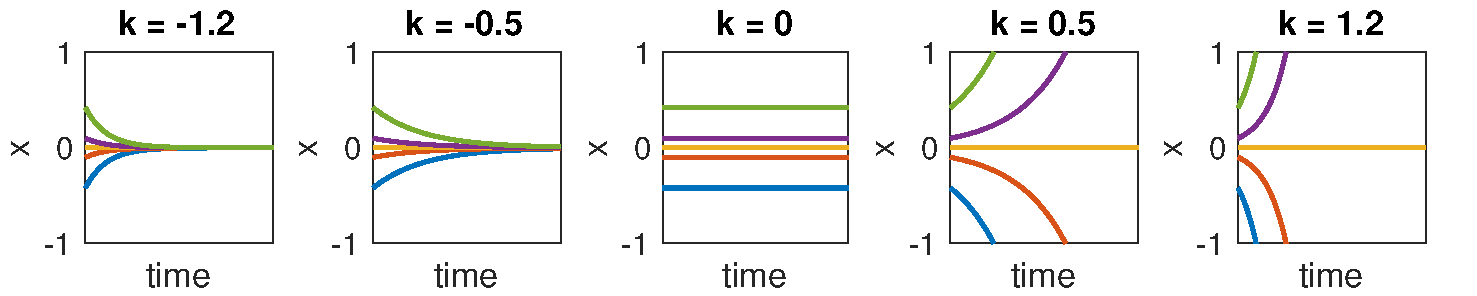
\includegraphics[width=\textwidth]{figures/ch3/evolution_of_straight_line2.pdf}
\caption[Evolution of the system given by the differential equation $\dot{x} = kx$ for different values of the control parameter $k$.]{Evolution of the system given by the differential equation $\dot{x} = kx$ for different values of the control parameter $k$. Colours indicate initial states: green = $0.42$, purple = $0.1$, yellow = $0$, red = $-0.1$, blue = $-0.42$.}
\label{fig:evolution_of_straight_line2}
\end{figure}

To learn about the patterns of the system without calculating solutions, a \emph{phase space plot} can be a useful tool \citep{Fuchs2013}. In a phase space plot it is particularly interesting to look for \emph{fixed points} -- points where the differential equation is zero, i.e. $\dot{x} = 0$. Figure \ref{fig:phase_space_straight_line} shows the phase space plots for $\dot{x} = kx$, for $k<0$ and $k>0$. The solutions for the system showed that nothing happens when $k = 0$, the system remains in its initial state. Hence, this case will not be discussed any further here and it will only be investigated what happens for $k < 0$ and $k > 0$. First, the left plot of Figure \ref{fig:phase_space_straight_line} is discussed where the control parameter $k$ is below zero. The function $\dot{x}$ has positive values for negative $x$ values, and negative values for positive $x$ values. Whenever the system is in a negative state (negative $x$), the change given by $\dot{x}$ is positive, so the system moves towards zero from the left side. Whenever the system is in a positive state (positive $x$), the change given by $\dot{x}$ is negative, so the system moves towards zero from the right side. This direction is indicated by the arrows on the x-axis. The further away the value of $x$ from zero, the greater the change -- this is shown by the size of the arrows. In addition, it is clear that $\dot{x} = 0$ for $x=0$. In sum, for $k<0$, when the system is at zero, it stays there; when it is in some other state (be it negative or positive), it gravitates towards zero. The black filled circle at zero indicates that zero is a \emph{stable fixed point} of the system, an attractor. 

\begin{figure}
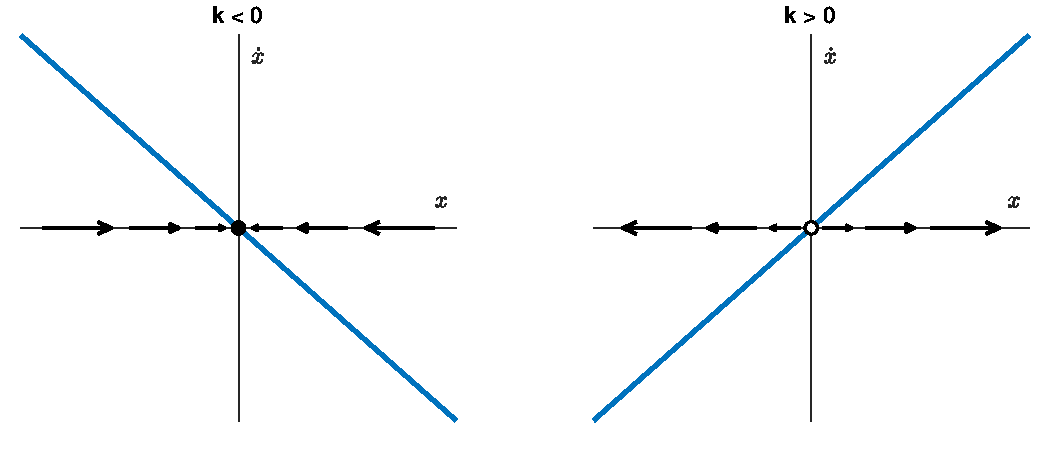
\includegraphics[width=\textwidth]{figures/ch3/straight_line.pdf}
\caption[Phase space plot of $\dot{x} = kx$.]{Phase space plot of $\dot{x} = kx$. Arrows indicate the direction of change in the system. The filled circle stands for attractor, the empty circle stands for repeller.}
\label{fig:phase_space_straight_line}
\end{figure}

In the right plot, the space phase plot is shown for cases in which the control parameter $k$ is greater than zero. Whenever the system is in a negative state (negative $x$), the change given by $\dot{x}$ is negative, so the system moves further away from zero towards $-\infty$. Whenever the system is in a positive state (positive $x$), the change given by $\dot{x}$ is positive, so the system moves further away from zero towards $\infty$. When the system starts at $x = 0$, it will stay there. But this is the only possibility to be in the state of zero for $k > 0$. All other initial states will lead away from zero, even states that are very close to zero, as for example $x = \frac{1}{10000}$. This is again indicated by the arrows, in this case pointing away from zero. Zero in this scenario is called an \emph{unstable fixed point} or \emph{repeller}, represented by an empty circle.

\medskip\noindent \textit{Code used in this section: ds\_straight\_line.m}

\subsection{Multistability}

Dynamical systems can have more than one attractor -- a situation called \emph{multistability}. Multistability is different to the ranges of control parameter values in the logistic map that exhibit a limit cycle attractor. In the case of the limit cycle, all values in the set of the attractor will be visited – the system oscillates between these values. The whole set is one attractor. In the case of a system with more than one attractor, the initial state is crucial in determining in which of the attractors the system will settle. At the end of this chapter, the concept of the stochastic dynamical system will be presented. In this case, random fluctuations play an important part and the role of the initial state in a multistable system is diminished.

The system that will be used here to illustrate the situation in which more than one attractor is present is the one defined by the differential equation in \ref{eq:double_well_force}, a system that will play a major role in this work. Figure \ref{fig:double_well_evolution} gives the solutions for some values of $k$ and some intitial states. Two aspects are important here: First, for $k = 0$ and $k = \pm0.2$, some trajectories settle in a positive attractor, others settle in a negative attractor. The attractor in which the system settles depends on the initial state. Second, for $k = \pm0.7$, the situation is different, the system only settles in one attractor regardless of the initial state.

\begin{equation}
\dot{x} = k + x - x^3
\label{eq:double_well_force}
\end{equation}

\begin{figure}
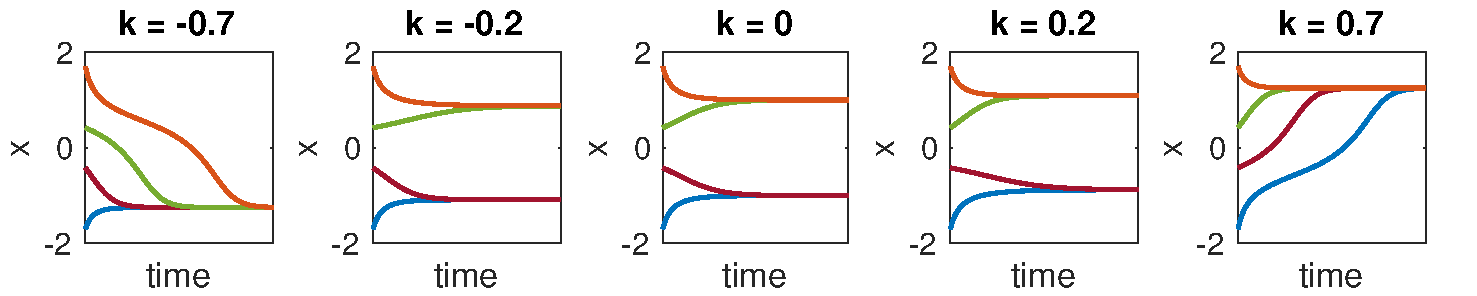
\includegraphics[width=\textwidth]{figures/ch3/evolution_of_double_well.pdf}
\caption[Evolution of the system given by the differential equation $\dot{x} = k + x - x^3$ with different control parameter $k$ values and different initial conditions.]{Evolution of the system given by the differential equation $\dot{x} = k + x - x^3$ with different control parameter $k$ values and different initial conditions. Colours indicate initial states: blue = $-1.7$; red = $-0.42$; green = $0.42$; orange = $1.7$.
}
\label{fig:double_well_evolution}
\end{figure}

The behaviour of this system can again be illustrated by the phase space plots \citep{Fuchs2013}, see Figure \ref{fig:double_well_force}. As before, an attractor is drawn as a full circle, a repeller is drawn as an empty circle. When the control parameter is zero, i.e. $k = 0$ (plot in the centre), two attractors and a repeller in the middle exist. When the control parameter is decreased (top row) or increased (bottom row), the attractor layout first remains as described until critical thresholds of the control parameter on both sides (increasing and decreasing) are reached. The symbols $-k_c$ and $+k_c$ stand for these critical values of the control parameter. When $k$ is smaller than $-k_c$, only one attractor exists, and this attractor is located in the negative range of the state axis. When $k$ greater than $k_c$, only one attractor exists in the system, and this attractor is located in the positive range of the state axis. 

When $k$ equals $-k_c$ or $k_c$, a \emph{half stable point} exists on the opposite side of the attractor, drawn as a square. This point acts like an attractor from one side but like a repeller from the other side. For example, when $k = -k_c$ (second plot in top row), the system will settle in this point when starting with an initial value that is greater than the location of this half stable point, i.e. coming from far right on the x-axis. On the contrary, when the initial state is a tiny bit to the left of the half stable point, the system will converge towards the attractor in the negative range on the x-axis.

In sum, this system exhibits bistability -- the presence of two attractors -- when $k$ is in the range between $-k_c$ and $k_c$ (i.e. $-k_c < k < k_c$). When the control parameter reaches the critical value on one or the other side ($-k_c$ or $k_c$), bifurcation occurs and the bistability breaks down: One attractor turns into a half-stable point at the respective critical threshold; beyond the critical values, even this half-stable point vanishes.

\begin{figure}
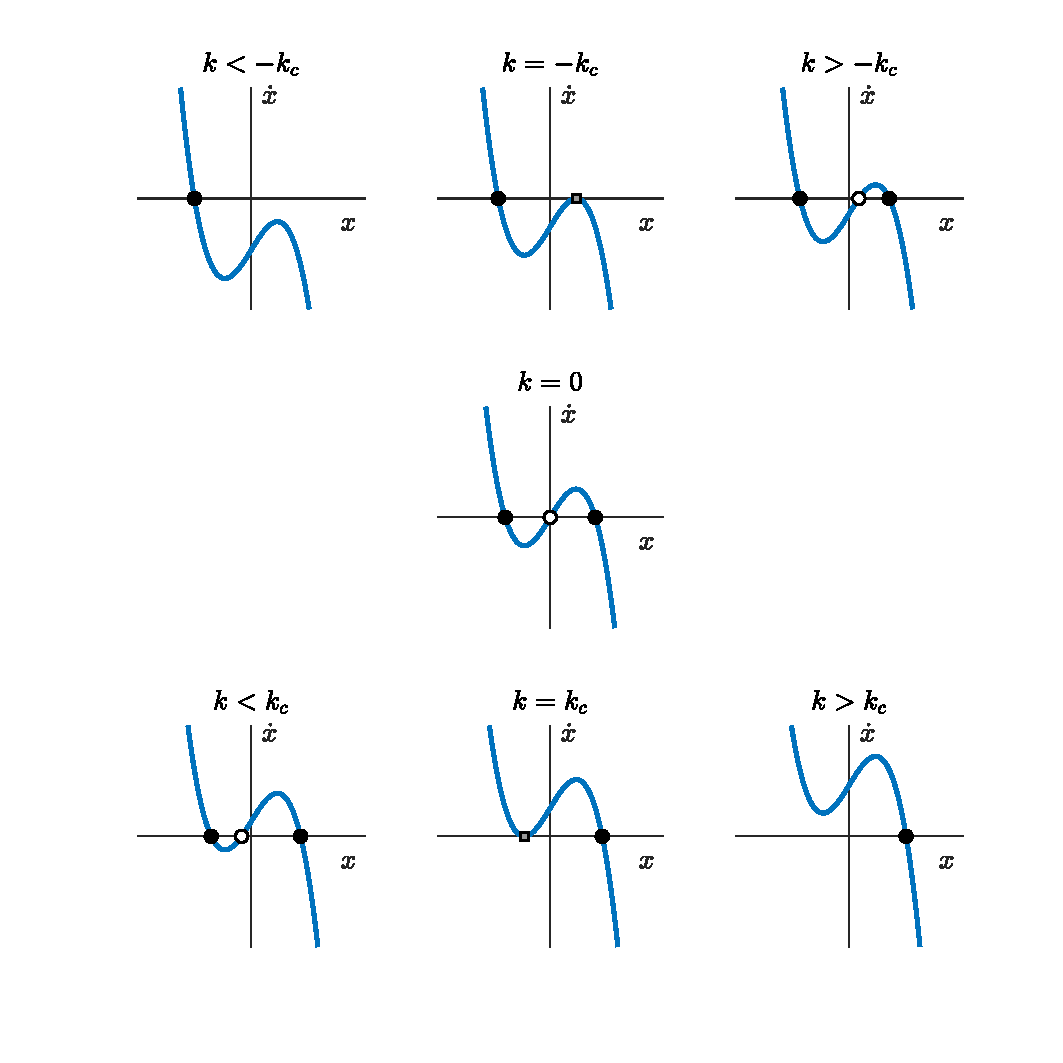
\includegraphics[width=\textwidth]{figures/ch3/double_well_force.pdf}
\caption[Phase space plot for $\dot{x} = k + x - x^3$.]{Phase space plot for $\dot{x} = k + x - x^3$. The filled circle stands for an attractor, the empty circle stands for a repeller, the square stands for a half-stable point.}
\label{fig:double_well_force}
\end{figure}

So far, differential equations have been used to represent a dynamical system. An additional, tightly connected way to define a dynamical system is by its \emph{potential function}. The potential is given by the negative integral of the differential equation. Thus, the relation of the differential equation, which is also often called the \emph{force function}, and the potential can be expressed as $\dot{x} = F(x) = -\frac{dV(x)}{dx}$, where $V(x)$ is the potential and $F(x)$ is the force. The graph of the potential function visualises the \emph{attractor landscape} of the dynamical system. Attractors appear as ``valleys", i.e. local minima in the graph. Figure \ref{fig:double_well_potential} gives the potential for the system defined by its differential in Equation \ref{eq:double_well_force}, the potential function itself is given in Equation \ref{eq:double_well_potential}. A commonly used metaphor for making the behaviour of the system understandable more intuitively is to imagine a ball or a marble rolling through the attractor landscape given by the potential \citep{HakenLevi2012}, since ``[t]he temporal evolution of a one-dimensional dynamical system corresponds to an overdamped motion of a particle in the landscape of its potential" \citep[22]{Fuchs2013}. Crucially, one has to think of the motion of the ball in ``thick or viscous fluid like honey" such that when ``it reaches a minimum it will stick there and will not oscillate back and forth" \citep[22]{Fuchs2013}.

\begin{equation}
V(x) = - kx - \frac{x^2}{2} + \frac{x^4}{4}
\label{eq:double_well_potential}
\end{equation}

Compare Figure \ref{fig:double_well_potential} (potential) to Figure \ref{fig:double_well_force} (force). When $k$ is zero, two symmetrical valleys are present in the potential. Because of this shape it is often called \emph{double-well potential}. Depending on where the ball starts, it rolls down either one of the valleys. When k is decreased or increased, the function tilts to one side, making one valley deeper and the opposite valley shallower. By passing the critical value of $k$ ($-k_c$ or $k_c$), one of the attractor valleys disappears -- in other words, the attractor becomes unstable and that state of the system ceases to be an attractor. Regardless of where the ball starts now, it will always roll into the remaining attractor. At the critical values, the ``fading attractor" takes an elbow shape. The ball metaphor can help to understand the fact that this point is half-stable: Suppose for instance that $k = -k_c$, if the ball starts on the right side of the half-stable point, it will roll down the potential to come to a halt at that point. If, on the contrary, it starts on the left side of the point, it will roll down to the attractor in the negative part of the x-axis. 

\medskip\noindent \textit{Code used in this section: double\_well.m}

\begin{figure}
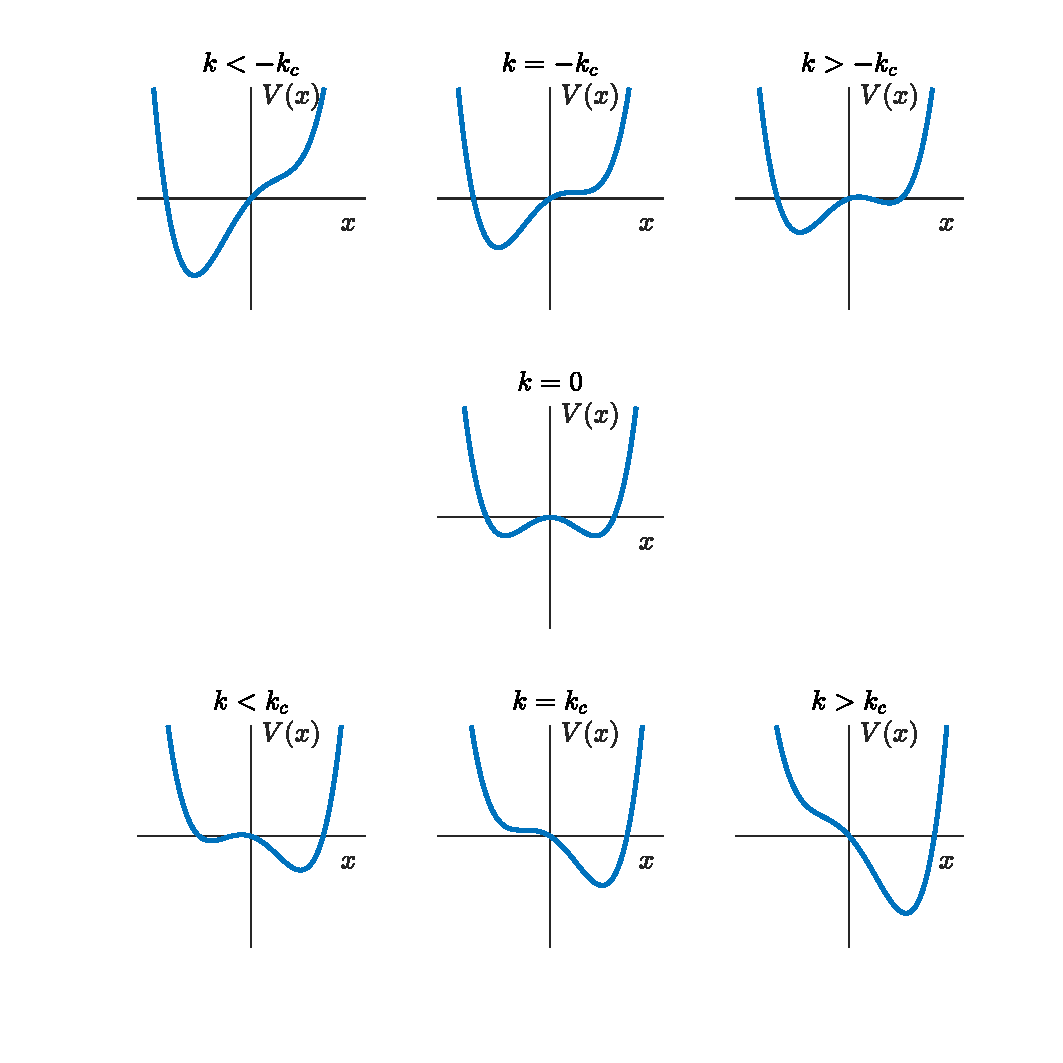
\includegraphics[width=\textwidth]{figures/ch3/double_well_potential.pdf}
\caption{Potential $V(x) = - kx - \frac{x^2}{2} + \frac{x^4}{4}$ corresponding to the phase space plots of the force $\dot{x} = k + x - x^3$.}
\label{fig:double_well_potential}
\end{figure}

\section{Applications of dynamical systems}

This chapter so far has outlined some of the basics of dynamical systems. In what follows, applications in the realm of human movement, language and speech will be discussed. This section presents a non-exhaustive collection of applications. The models are explained in some detail as they provide inspiration for the modelling approach presented in the second part of the book.

\subsection{Modelling coordination and speech dynamics}

Patterns of human motion have been fruitfully described in terms of dynamical systems. Since speech production represents a highly intricate system of coordinated movements, a large and growing body of research has applied nonlinear dynamics to speech. The present subsection introduces and highlights some interesting points of this research.

\subsubsection{Inter-limb coordination}

An influential application of dynamical systems in the domain of human behaviour is the model of \citet{HakenKelsoBunz1985}. This model presents a mathematical description of interesting observations on the coordination patterns of finger movements made in earlier research by one of the authors. In the study of \citet{Kelso1981}, the subjects moved the index fingers of both hands simultaneously at varying frequencies. One remarkable finding was that subjects were able to coordinate the movements of their fingers in two different stable modes: anti-symmetrically, a coordination pattern also known as \emph{anti-phase}, or symmetrically, a coordination pattern known as \emph{in-phase}. These two modes are illustrated in Figure \ref{fig:hkb_fingers}.

\begin{figure}
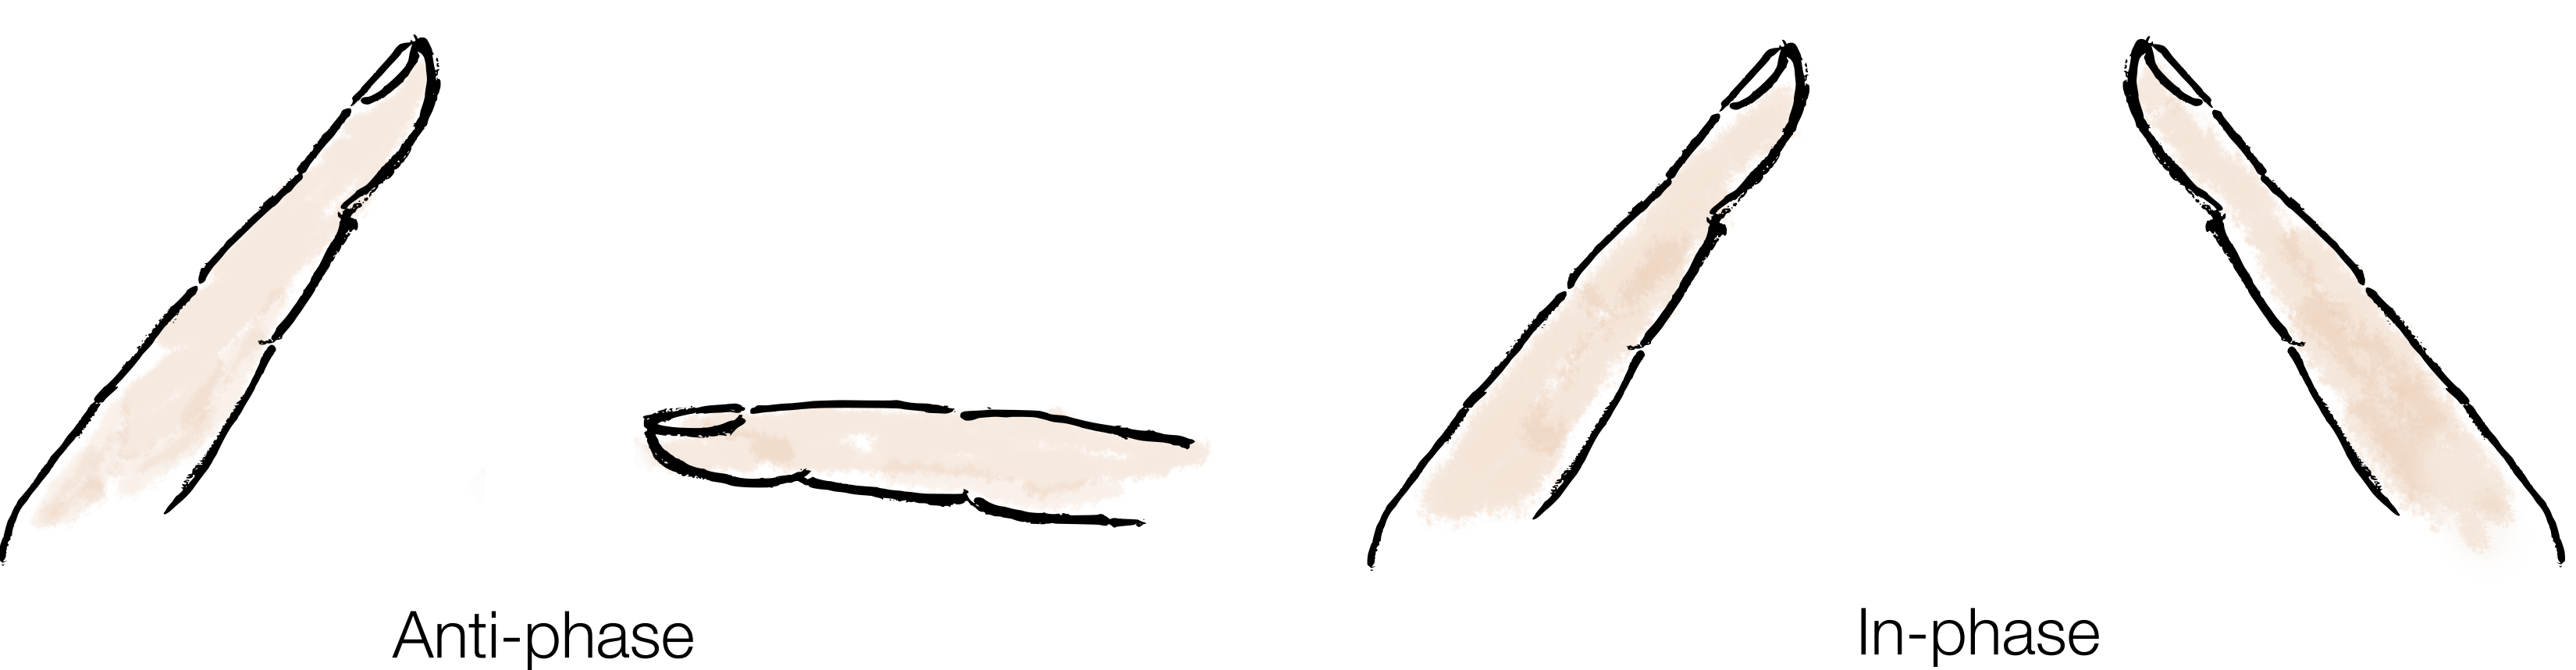
\includegraphics[width=11cm]{figures/ch3/hkb_fingers.png}
\caption[Stable coordination patterns found in \citet{Kelso1981}.]{Stable coordination patterns found in \citet{Kelso1981} and used for the modelling approach in \citet{HakenKelsoBunz1985}: anti-phase vs. in-phase.}
\label{fig:hkb_fingers}
\end{figure}

In terms of a dynamical model, the movement of each finger can be idealised as a harmonic oscillation and each oscillation can be described by its phase angle $\phi_i$ \citep{HakenKelsoBunz1985}. When modelling the coordination patterns introduced in the last paragraph, the \emph{relative phase} is of primary concern. Let $\phi_1$ and $\phi_2$ be the phase angles of the respective fingers, then $\phi = \phi_2 - \phi_1$ is the relative phase. In the right panel of Figure \ref{fig:hkb_phase_position}, the oscillations of the two fingers in anti-phase (top) and in-phase (bottom) are shown.\footnote{The oscillations for both fingers have identical frequencies and amplitudes in this example.} The dashed line marks one time point $t_1$. The left panel gives the phase angles of the oscillations at this time point $t_1$. When the oscillations of the fingers are in anti-phase mode (top), the phase angles are displaced by 180°, i.e. the relative phase $\phi$ is 180°. At $t_1$, $\phi_1$ is 40° and $\phi_2$ is 220° and consequently $\phi=\phi_2-\phi_1=180$°. The relative phase is visualised by the grey shaded circular sector in the phase angle plot on the left. When the oscillations of the fingers are in in-phase mode (bottom), their phase angles are identical and the relative phase is 0°. At $t_1$ in the lower panel, both $\phi_1$ and $\phi_2$ are 220°, hence $\phi = \phi_2 - \phi_1 = 0$°. When plotted on top of each other, only one of the oscillations is visible in this case. 

\begin{figure}
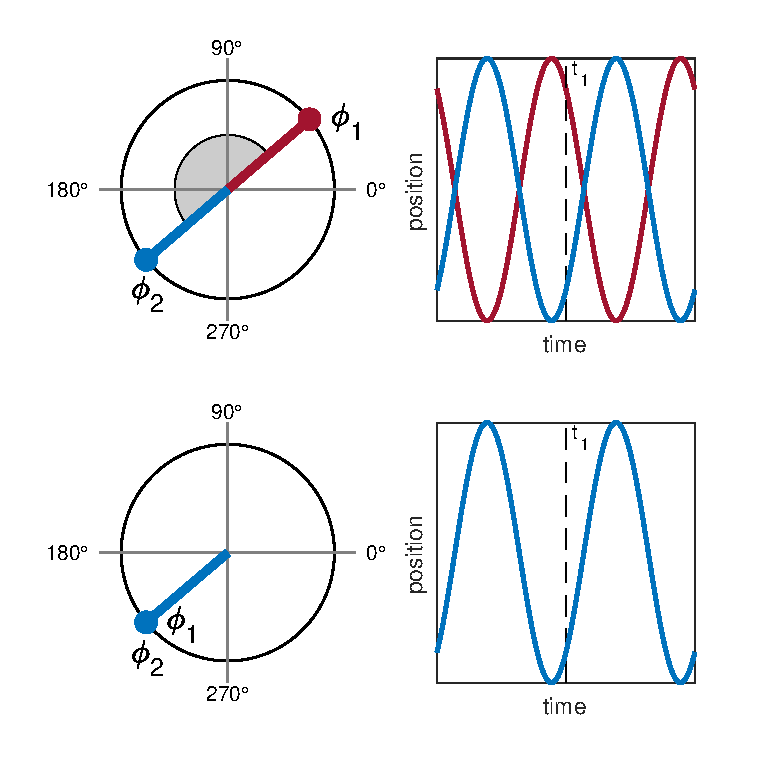
\includegraphics[width=10cm]{figures/ch3/phase_position_hkb_fingers.pdf}
\caption{Phase angles and evolution of the oscillatory finger movements as modelled by \citet{HakenKelsoBunz1985}.}
\label{fig:hkb_phase_position}
\end{figure}

An additional result of \citet{Kelso1981} was that when subjects started to move their index fingers in anti-phase (as in the top panel of \ref{fig:hkb_phase_position}) and the frequency of this movement was increased, the subjects' finger movements changed abruptly to an in-phase coordination (as in the bottom panel of \ref{fig:hkb_phase_position}) at a critical frequency boundary. To capture these findings, \citet{HakenKelsoBunz1985} proposed a model that has attractors for anti-phase and in-phase coordination for certain ranges of the control parameter and a single attractor for in-phase coordination when the control parameter is scaled past a critical threshold. The model is given by its potential energy function in Equation \ref{eq:hkb_potential}. The control parameter is the ratio of $b$ and $a$, i.e $\frac{b}{a}$. The potential is in fact periodic and so the shape of the attractor landscape repeats over and over again with $V(\phi + 2\pi) = V(\phi)$. 

\begin{equation}
V(\phi) = -a \cos(\phi) - b \cos( 2 \phi)
\label{eq:hkb_potential}
\end{equation}

In the model, increasing frequency of the movements is conceptualised as a decrease in the ratio $\frac{b}{a}$. Figure \ref{fig:hkb_landscapes} illustrates the attractor landscapes for different values of the $\frac{b}{a}$. To interpret the effect of scaling $\frac{b}{a}$ towards zero, the metaphor of a ball rolling down the attractor landscape can be employed again. In the figure, the ball starts in one of the anti-phase attractors with $\frac{b}{a} = 1$ (top left). This attractor is at $\phi = \pi$ which is the phase angle of 180° in radians. When going from left to right and top to bottom in the plot, the tempo of the finger movement increases and the ratio $\frac{b}{a}$ decreases. However, at first, the ball stays in the initial anti-phase attractor. This attractor basin becomes shallower until it is not an attractor basin anymore. At this critical value of $\frac{b}{a}$ (see lower left corner), the ball will be set into motion and roll down to the in-phase attractor which is at $\phi = 0$.

\begin{figure}
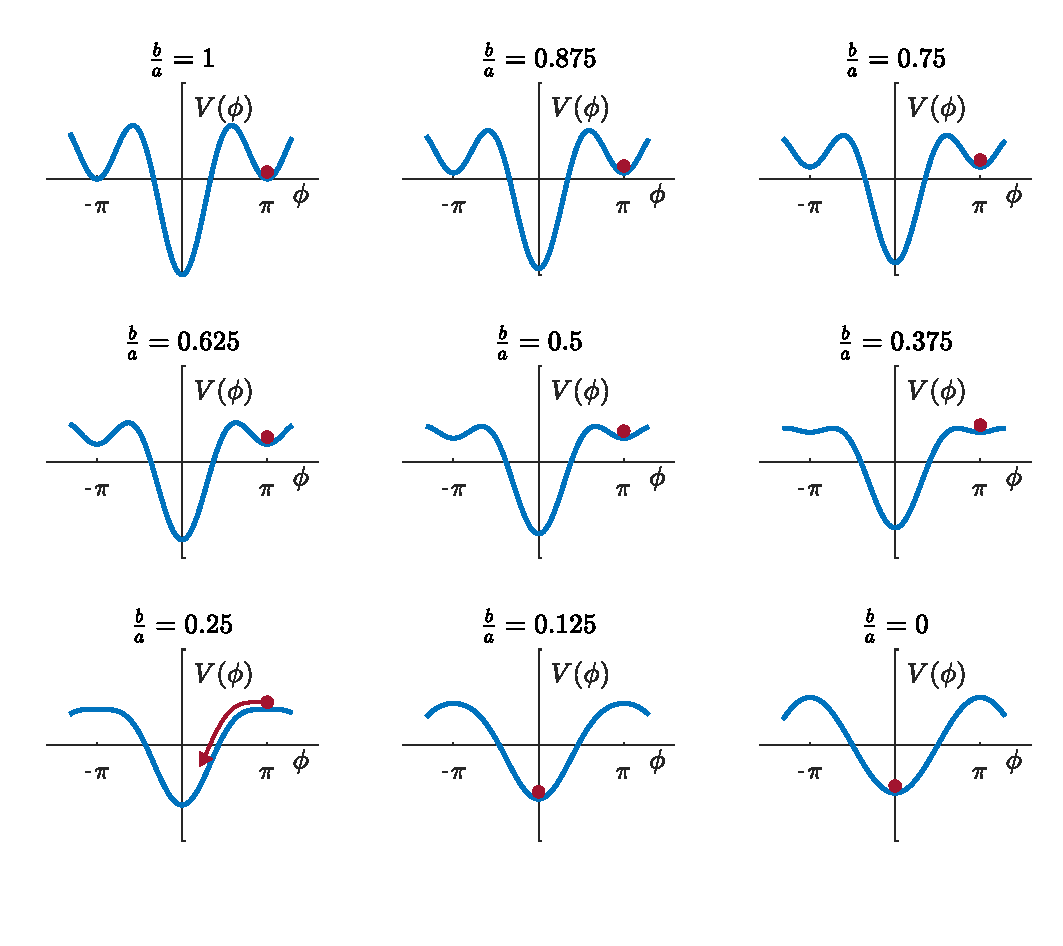
\includegraphics[width=\textwidth]{figures/ch3/hkb_potential.pdf}
\caption{Attractor landscapes of \citet{HakenKelsoBunz1985} for different values of $\frac{b}{a}$.}
\label{fig:hkb_landscapes}

\end{figure}

Figure \ref{fig:hkb_simulation} shows what happens to the oscillatory finger movements (upper pannel)  and their relative phase (middle panel) over time when the ratio $\frac{b}{a}$ drops beyond the critical value. As can be seen in the middle panel, the relative phase changes from anti-phase to in-phase abruptly -- with a small portion of instability after which the oscillations of the fingers in the top panel are exactly synchronous (and thus plotted on top of each other).

Hence, this dynamical model that is able to account for two qualitatively distinct coordination modes of finger motion using a potential function that is modulated by scaling a continuous parameter (or the ratio of two parameters). The model was in fact seminal and had great impact on models of speech production as will become clear in what follows. First, a closer look at the use of dynamics to model the \emph{gesture} in Articulatory phonology will be taken. Second, the coupled oscillator model for \emph{intergestural coordination} building upon \citet{HakenKelsoBunz1985} will be presented.

\begin{figure}
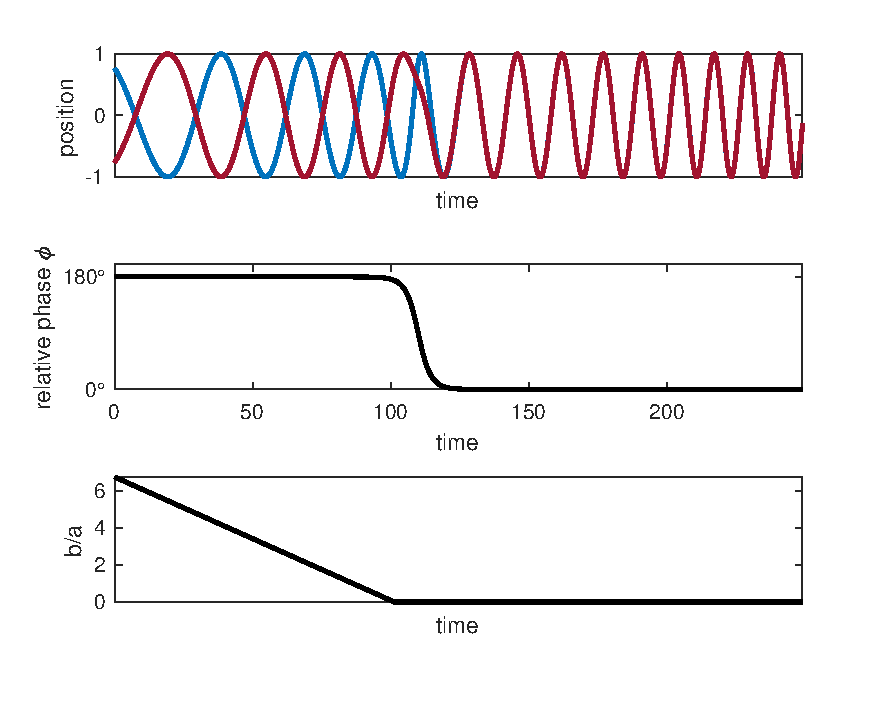
\includegraphics[width=12cm]{figures/ch3/hkb_simulation.pdf}
\caption{Simulation of the model of \citet{HakenKelsoBunz1985} starting in anti-phase mode and turning into in-phase mode.}
\label{fig:hkb_simulation}
\end{figure}

\medskip\noindent \textit{Code used in this section: hkb\_phase\_modes.m, hkb\_potential.m, hkb\_simulation.m}


\subsubsection{Articulatory gestures}

The framework of Articulatory phonology, as described in Chapter \ref{chapter_pandp}, views gestures as the primitives of phonology. Gestures are orchestrated to build higher forms like syllables and words. A gesture is defined in terms of a dynamical model. Chapter \ref{chapter_pandp} outlined how the model is able to account for variation in the speech signal, as for example the case of assimilation. In the current chapter, the model will be reviewed from the dynamical perspective.

Articulatory phonology builds upon a model known as \emph{task dynamics} to describe the gestures of speech production. Task dynamics (see \citealp{Saltzman1986, SaltzmanKelso1987, Saltzman1991}; as well as \citealp{Hawkins1992} for an introductory overview) has been developed to describe various patterns of movement that include multiple effectors like the shoulder, the upper and lower arm as well as the hand when grasping an object. Similar to other motion systems, speech involves the coordination of multiple effectors, in this case articulators, to form the relevant constrictions \citep{BrowmanGoldstein1989}. The task dynamics approach to articulation does not focus on the motion of the individual articulators but on the motion of \emph{tract variables} \citep{BrowmanGoldstein1992}. Tract variables describe the coordinative structures that jointly yield the relevant constrictions. For example, the upper lip, the lower lip and the jaw contribute to the tract variable of lip aperture \citep{BrowmanGoldstein1992}. Table \ref{tab:tract_vars} gives an overview of the tract variables and the articulators involved in these tract variables. Most tract variables come in “horizontal-vertical” pairs: Constriction location (horizontal) is combined with constriction degree (vertical). The gestures in Articulatory phonology are formed from the set of tract variables. When constriction degree and location are present, both dimensions are used to build the gesture.

\begin{table}
\caption{Tract variables of Articulatory phonology from \citet[73]{BrowmanGoldstein1989}.}
\begin{tabularx}{\textwidth}{Xll}
	\lsptoprule
&			\textbf{tract variable} &			\textbf{articulators involved}\\
\midrule
\textbf{LP} &		lip protrusion &				upper and lower lips, jaw\\
\textbf{LA} &		lip aperture &				upper and lower lips, jaw\\
\textbf{TTCL} &	tongue tip constriction location &	tongue tip, body, jaw \\
\textbf{TTCD} &	tongue tip constriction degree &		tongue tip, body, jaw \\
\textbf{TBCL} &	tongue body constriction location &	tongue body, jaw \\
\textbf{TBCD} &	tongue body constriction degree &	tongue body, jaw \\
\textbf{VEL} &	velic aperture &				velum \\
\textbf{GLO} &	glottal aperture &				glottis \\
  \lspbottomrule
\end{tabularx}
\label{tab:tract_vars}
\end{table}%

At the heart of the modelling approach of task dynamics is a dynamical system known as the \emph{damped harmonic oscillator} that specifies the control of a tract variable \citep{Hawkins1992}. It is formulated mathematically as the second order differential equation given in Equation \ref{eq:dho} \citep{SaltzmanKelso1987}. The systems reviewed in this chapter so far were given by first-order differential equations. In a second-order differential equation the second derivative, denoted by $\ddot{x}$, occurs.

\begin{equation}
m\ddot{x} + b\dot{x} + k(x-x_0) = 0
\label{eq:dho}
\end{equation}

The damped harmonic oscillator describes the motion of a mass attached to a spring that is stretched vertically \citep{FeynmanLeightonSands1963}, and is therefore often referred to as a spring-mass system. The state variable $x$ is the position of the mass attached to the spring, $\dot{x}$ is its velocity and $\ddot{x}$ is its acceleration. Besides $x$ and its two derivatives, a collection of parameters occurs in the equation: $m$, $b$, $k$ and $x_0$. These parameters are discussed shortly in this section; examples are given to illustrate the consequences of manipulating the parameters. 

The parameter $m$ refers to the mass attached to the spring. This parameter is usually set to 1 and not changed. For the sake of completeness, however, Figure \ref{fig:dho_mass}  shows what happens when the mass is changed (for this simulation, the parameter $b$ is set to 0, the parameter $k$ is set to 1, the parameter $x_0$ is set to 0). For higher values of $m$, the system oscillates at lower frequencies. It is easy to understand intuitively that greater masses need more time to be transported over the same distance compared to smaller masses. 

\begin{figure}[htp]
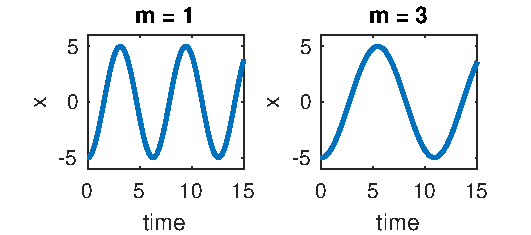
\includegraphics[width=7cm]{figures/ch3/dho_mass.pdf}
\caption{Consequences of scaling the parameter $m$ (mass) in the harmonic oscillator.}
\label{fig:dho_mass}
\end{figure}

The same effect is achieved by changing the parameter $k$, the stiffness of the spring, as shown in Figure \ref{fig:dho_stiff} (for this simulation, the parameter $b$ is set to 0, the parameter $m$ is set to 1, the parameter $x_0$ is set to 0). For higher values of $k$ the system oscillates at higher frequencies. Here as well, an intuitive understanding is facilitated by imagining the consequences of pulling two springs which differ with regard to their stiffness: The stiffer spring snaps back faster.

\begin{figure}
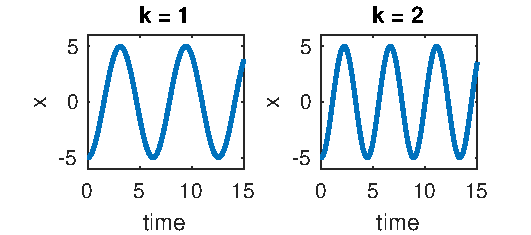
\includegraphics[width=7cm]{figures/ch3/dho_stiffness.pdf}
\caption{Consequences of scaling the parameter $k$ (stiffness) in the harmonic oscillator.}
\label{fig:dho_stiff}
\end{figure}

More important for the modelling of articulatory gestures is the parameter $b$, the damping of the system. Damping leads to dissipation of energy stored in the system due to friction and reduces (or even prevents) the system’s oscillation. Figure \ref{fig:dho_damp} illustrates four interesting cases of damping. In all cases, the mass $m$ and the stiffness $k$ are set to 1, $x_0$ is set to 0. In the top left plot, the undamped case is shown, $b = 0$. The system is \emph{not} damped, just like in the plots illustrating the changes of mass and stiffness. In this case, the system will oscillate forever. In the top right plot, the case of an \emph{underdamped} system is shown. The system oscillates but the amplitudes shrink and the system converges towards a resting position. In the bottom panels, the cases of a \emph{critically damped} system (left) and an \emph{overdamped} system (right) are illustrated. In these cases, the system does not oscillate and converges towards a resting position, similar to the constant growth model $\dot{x} = kx$ for $k<0$ discussed above.

\begin{figure}
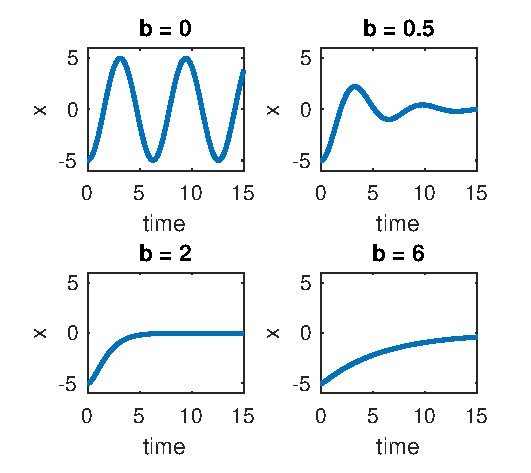
\includegraphics[width=7cm]{figures/ch3/dho_damping.pdf}
\caption{Consequences of scaling the parameter $b$ (damping) in the harmonic oscillator.}
\label{fig:dho_damp}
\end{figure}

\hspace*{-1mm}Finally, $x_0$ denotes equilibrium or resting position. Figure \ref{fig:dho_rest} gives an over\-view of the consequences of manipulating this parameter for a critically damped system. As illustrated by the plots, for a critically damped system or an overdamped system, the parameter $x_0$ is the position of the point attractor that the system converges to. In Articulatory phonology, the control of a tract variable is modelled with a critically damped harmonic oscillator. The resting position $x_0$ corresponds to the constriction location or degree depending on the tract variable. 

\begin{figure}
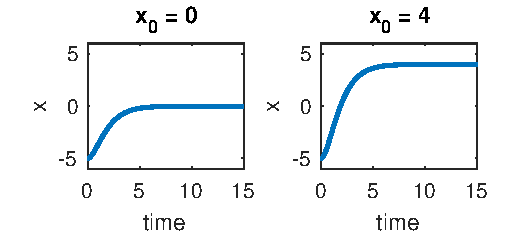
\includegraphics[width=7cm]{figures/ch3/dho_x0.pdf}
\caption{Consequences of scaling the parameter $x_0$ (equilibrium position) in the harmonic oscillator.}
\label{fig:dho_rest}
\end{figure}

In fact, a critically damped harmonic oscillatory never reaches its resting position but only approaches it infinitesimally close. For a concrete implementation scenario of the model, a point has to be defined at which the target is said to be reached. As shown above, an undamped oscillator repeats in even cycles and its oscillation can be described by the phase angle as already shown for the finger movements when discussing the \citet{HakenKelsoBunz1985} model. Articulatory phonology defines the target of the critically damped oscillator as the point of 240° of the undamped corresponding oscillator \citep{BrowmanGoldstein1990}, as shown in Figure \ref{fig:dho_240}. In this figure, one full undamped oscillator cycle is plotted as a solid red line, and the corresponding undamped oscillator is plotted as a dotted blue line. The vertical black line indicates the point where a phase angle of 240° is reached in the cycle of the undamped oscillator, i.e. the \emph{target} of the gesture described by the damped harmonic oscillator. The second x-axis on the bottom relates the time points on the first x-axis to the phase angles in degrees.

\medskip\noindent\textit{Code used in this section: \\
damped\_harmonic\_oscillator.m, damped\_harmonic\_oscillator\_target.m}

\begin{figure}
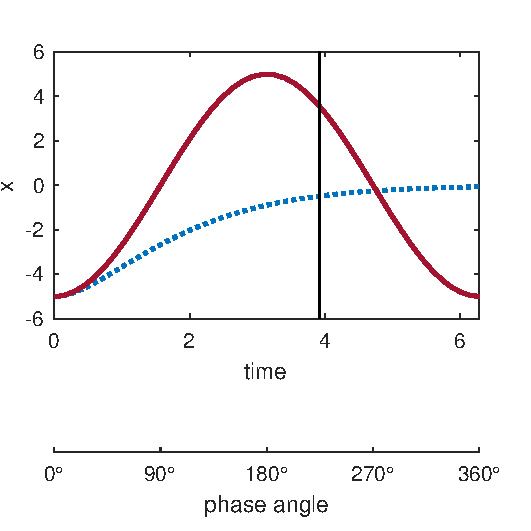
\includegraphics[width=7cm]{figures/ch3/target_240_degrees.pdf}
\caption{The target of the critically damped harmonic oscillator is reached at 240° of the phase angle of the corresponding undamped oscillator.}
\label{fig:dho_240}
\end{figure}

\subsubsection{Inter-gestural timing}

Articulatory phonology views words and syllables as made up of gestures. Although timely ordered in some sense, these gestures are, crucially, not ``beads on string" \citep{Pouplier2011}, i.e. they are not strictly sequentially ordered. Structures like words and syllables should rather be seen as molecular structures \citep{NamGoldsteinSaltzman2009} consisting of gestures and connections between the gestures that determine their relative timing. This section will shed some light on the modelling of timing in Articulatory phonology. Here again, a dynamical systems approach is used which will be reviewed in some detail since it ties together what has been presented in the last two sections on the \citet{HakenKelsoBunz1985} model and the modelling of gestures in Articulatory phonology. 

It has been highlighted in different passages of this work that \emph{timing} is important in the context of  modelling articulatory gestures. The gestural score in Figure \ref{fig:score_late_calls} in Chapter \ref{chapter_pandp} emphasised this fact by showing how fine-grained timing differences can account for more subtle processes, like for example assimilation. To illustrate the point in the present context and for the sake of completeness and clarity, another gestural score is presented in Figure \ref{fig:ban_mad} for the words \emph{ban} and \emph{mad}, adapted from \citet{Goldsteinetal2009}. The only difference between the scores is the timing of the \emph{velar wide} gesture. The result are two completely different words. This simple example demonstrates that the relative timing of the gestures (i.e. the timing of a gesture in relation to another gesture) involved in forming the word plays a significant role in determining phonological structures and lexical contrast. 

\begin{figure}
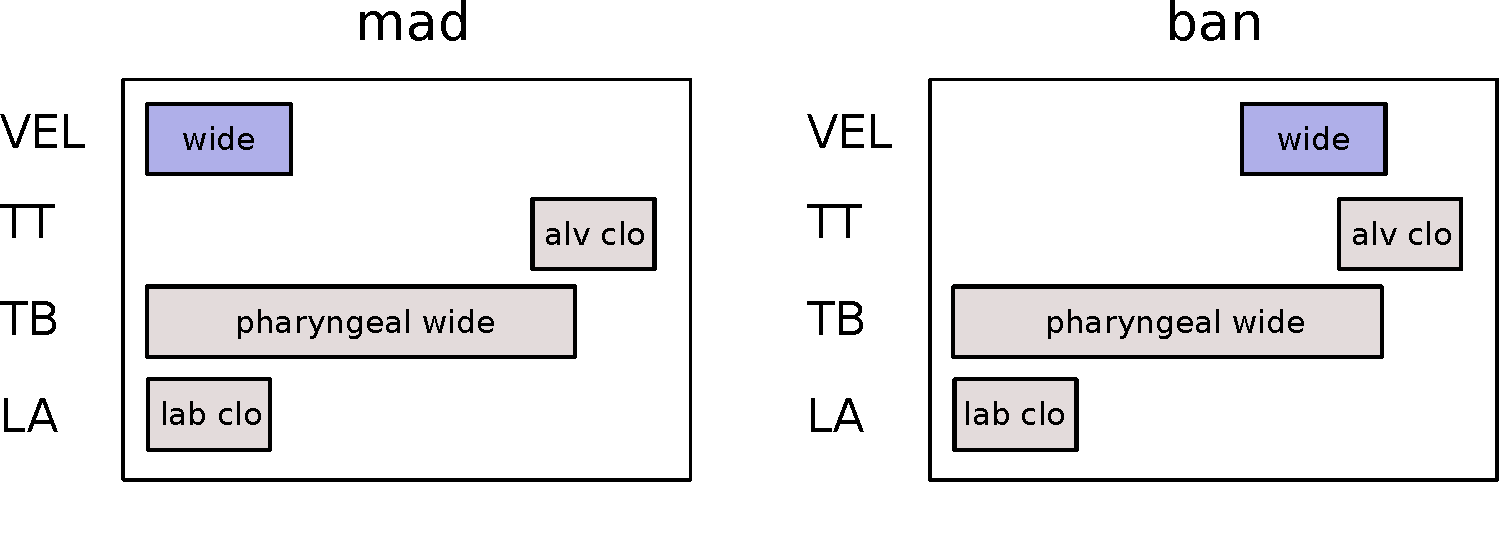
\includegraphics[width=11cm]{figures/ch3/ban_mad.pdf}
\caption{Gestural scores for the words \emph{ban} and \emph{mad} adapted from \citet{Goldsteinetal2009}.}
\label{fig:ban_mad}
\end{figure}

The timing structure of articulatory gestures has been described in detail in a model using \emph{coupled oscillators} \citep{SaltzmanByrd2000, NamSaltzman2003, Goldsteinetal2009, Tilsen2017}. The central idea of this model is that each gesture is associated with a planning oscillator. This planning oscillator is not to be confused with the oscillator that describes the trajectory of the gesture itself. The planning oscillators of multiple gestures are connected with a coupling relation that determines the relative phases of the gestures. As in the model of \citet{HakenKelsoBunz1985}, the two stable patterns of the relative phasing are in-phase and anti-phase. During planning, the oscillators adjust their phases either in an in-phase or anti-phase manner. When a stable pattern is achieved, the actual production gestures are activated by the oscillators. The adjustment of the oscillators towards a stable pattern is modelled using a potential function similar to that of \citet{HakenKelsoBunz1985}. There exist slightly different ways to formulate the coupled oscillator model \citep{SaltzmanByrd2000, Tilsen2017}. \citet{Tilsen2017} presents the potential functions as formulated in \ref{eq:coupled_osc_potential}, where $V^+$ is the potential for  in-phase coupling and $V^-$ is the potential for anti-phase coupling (as in the model of \citeauthor*{HakenKelsoBunz1985}, $\phi$ is relative phase of the oscillators, given as the difference between the individual phases $\theta$: $\phi_{ij} = \theta_i - \theta_j$). The evolution of the relative phase  can be described using the negative derivative of the potential, the force function of the system, as given in Equation \ref{eq:coupled_osc_force}.

\begin{equation}
\begin{split}
V^+(\phi) = -\cos\phi, \quad\quad
V^-(\phi) = \cos\phi
\label{eq:coupled_osc_potential}
\end{split}
\end{equation}

\begin{equation}
F(\phi) = -\frac{dV(\phi)}{d\phi}
\label{eq:coupled_osc_force}
\end{equation}

Each planning oscillator $i$ can be expressed in polar coordinates with the phase $\theta_i$ such that the evolution of planning oscillator's phase without coupling can be described as in Equation \ref{eq:coupled_osc_phase_angle}, where $f_i$ represents the intrinsic frequency of the oscillator \citep{Tilsen2018}.

\begin{equation}
\dot{\theta_i} =  2 \pi f_i
\label{eq:coupled_osc_phase_angle}
\end{equation}

To model the effect of coupling, the expression of Equation \ref{eq:coupled_osc_phase_angle} that models the evolution of the phase angle is extended by the force function of the coupling dynamics $F(\phi)$, see Equation \ref{eq:coupled_osc_phase_angle_with_coupling} \citep{Tilsen2017}. The force that is exerted on the planning oscillator is proportional to the coupling strengths of the planning oscillators. These coupling strengths are given as a matrix in which the coupling strength of each planning oscillator $i$ to another oscillator $j$ is defined. This matrix for three coupled oscillators looks like the one given in Equation \ref{eq:coupled_osc_matrix}. The diagonal elements $c_{ii}$ of the matrix are $0$ because they denote the coupling of the oscillator to itself.

\begin{equation}
\dot{\theta_i} =  2 \pi f_i + \sum_j{ c_{ij} \frac{-dV(\phi_{ij})}{d\phi_{ij}}}
\label{eq:coupled_osc_phase_angle_with_coupling}
\end{equation}

\begin{equation}
C = 
\begin{pmatrix}
0 & c_{12} & c_{13} \\
c_{21} & 0 & c_{23} \\
c_{31} & c_{32} & 0 \\
\end{pmatrix}
\label{eq:coupled_osc_matrix}
\end{equation}

Figure \ref{fig:coupled_oscillators} provides an example of two oscillators that are coupled in an in-phase manner and that start with a relative phase of 110°. The three rows of the figure show three different points in time. The first row presents a time point that is shortly after the beginning of the simulation, the relative phase at this time point is still close to the initial relative phase of 110°. The last row presents a time point at which the two oscillators have almost the same phase, i.e. the relative phase is close to 0°. The middle row presents a time point in between. In the left column, the graph of the potential function is shown with the red dot indicating the current state of the system (it is possible to think of the dot as the ball in the metaphor used above). In the mid column, the phase angles of the oscillators are presented. In the right column, the position of the oscillators are shown in a time window around the time point corresponding to the potential and the phase angles in the same row (the dashed line specifies this time point). The plot illustrates how the state of the system approaches the attractor at 0°, the minimum of the potential, and how the relative phase of the two oscillators decreases over time. 

\begin{figure}
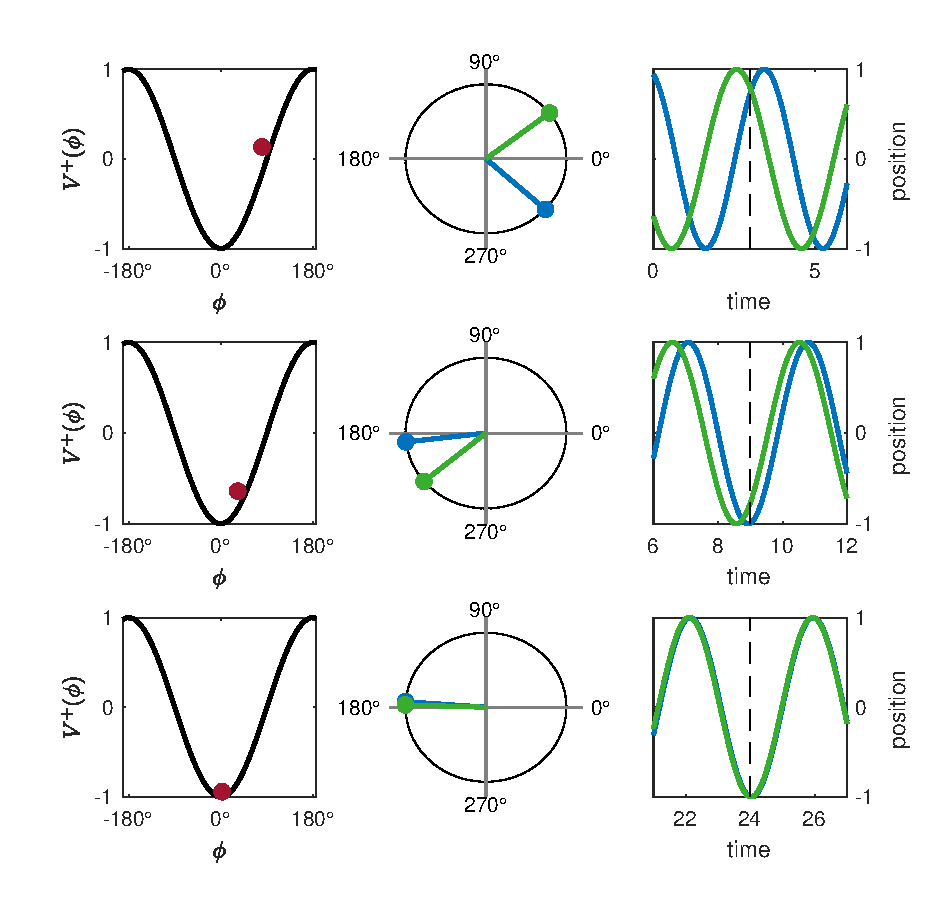
\includegraphics[width=\textwidth]{figures/ch3/coupled_oscillators.pdf}
\caption[Potential, phase angles and position corresponding to two oscillators coupled in-phase]{Potential, phase angles and position corresponding to two oscillators coupled in-phase at three time points (from top to bottom).}
\label{fig:coupled_oscillators}
\end{figure}

Usually, syllables involve more than two gestures and, thus, more than two oscillators are coupled in a pair-wise fashion. As a result, a network of coupled oscillators emerges.\footnote{An alternative view is that the oscillator of each gesture is coupled to a master clock. This perspective is discussed in relation to the network of coupled oscillators in \citet{Goldsteinetal2009}.} The target phasing relations of these oscillators are represented in \emph{coupling graphs}. The coupling graphs for the English words \emph{bud} [bʌd] and \emph{dub} [dʌb], adapted from \citet{Mücke2018}, are shown in Figure \ref{fig:bud_dub}. The solid lines indicate in-phase coupling, the dashed lines indicate anti-phase coupling. The onset consonant of the syllable in both cases is modelled as being coupled in-phase with the vowel of the syllable while the coda consonant is coupled anti-phase with the vowel. This organisation reflects the fundamental hypothesis that CV structures in a syllable are coupled in-phase while VC structures are coupled anti-phase \citep{GoldsteinByrdSaltzman2006, Goldsteinetal2009}.

\begin{figure}
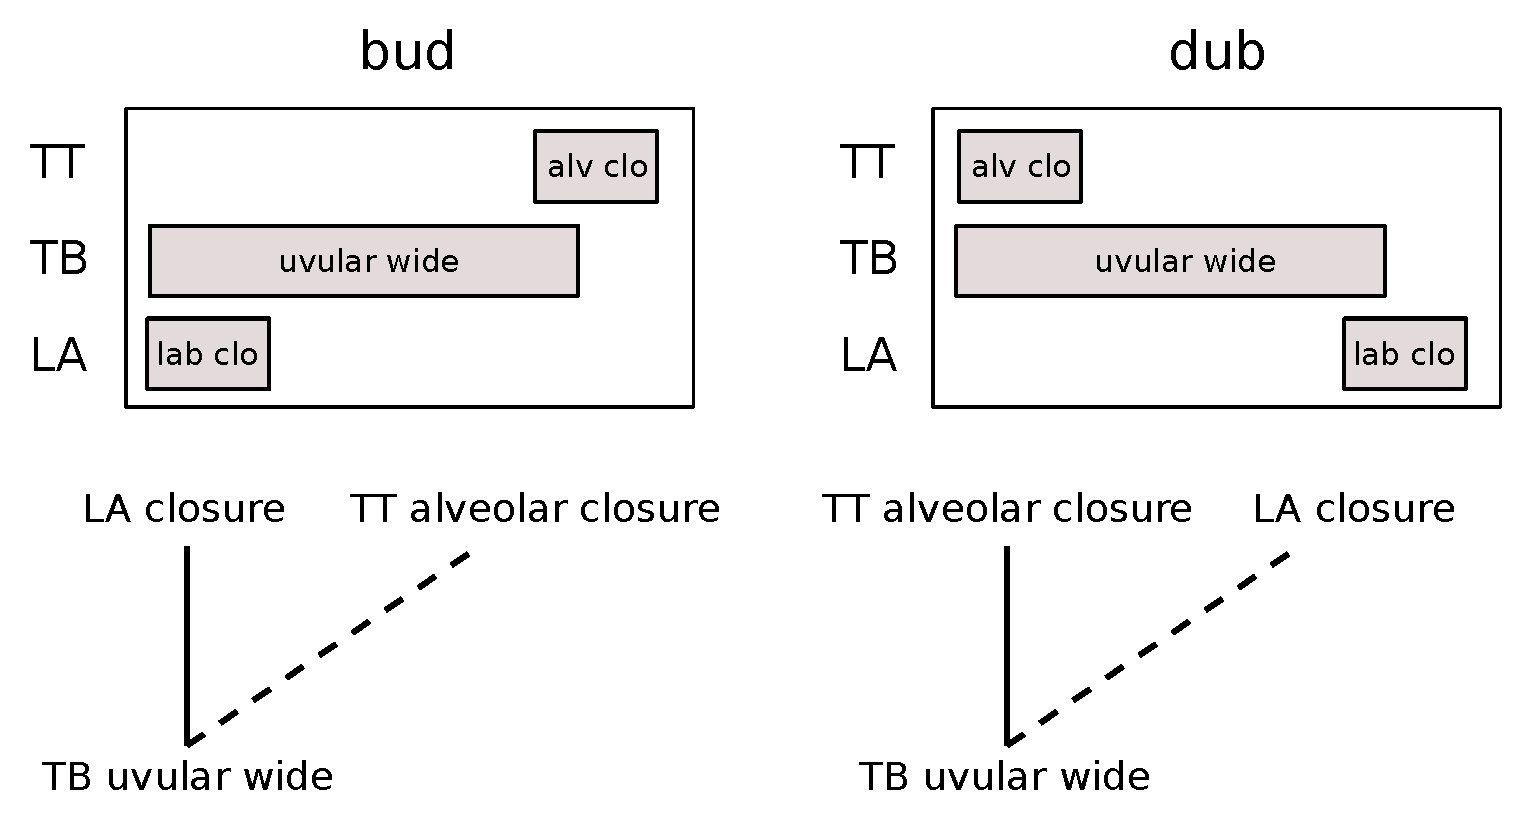
\includegraphics[width=11cm]{figures/ch3/bud_dub.pdf}
\caption[Gestural scores and coupling graphs for \emph{bud} and \emph{dub}.]{Gestural scores and coupling graphs for \emph{bud} [bʌd] and \emph{dub} [dʌb] adapted from \citet{Mücke2018}, solid lines indicate in-phase coupling, dashed lines indicate anti-phase coupling.}
\label{fig:bud_dub}
\end{figure}

If two consonants or more are present in the onset of a syllable, a pair-wise in-phase coupling of all of the consonants to the vowel alone would lead to an overlapping of the consonants. To achieve at least a partially sequential realisation of the onset consonants, the onset gestures of each consonant can be coupled with anti-phase links to the vowel. The result is a \emph{competitive coupling} in which the final phases represent a compromise of the competing coupling forces \citep{Nam2007, Saltzmanetal2008, Goldsteinetal2009}. Competitive coupling is able to explain an effect known as the \emph{C-centre effect} in branching onsets \citep{BrowmanGoldstein1988, Byrd1995}. The C-centre effect, illustrated in Figure \ref{fig:c-centre}, describes the following situation: The timing of C1 in relation of the vowel V in a complex onset structure C1C2V is earlier compared to the simple structure C1V. In other words, when a second consonant C2 is added after C1, the earlier consonant C1 shifts leftwards. Likewise, the timing of C2 in C1C2V is later compared to the simpler structure C2V, i.e. when a second consonant C1 is added before C2, the later consonant C2 shifts rightwards. The timing of the centre of the consonant cluster in relation to the vowel, however, stays constant \citep{BrowmanGoldstein1988, Goldsteinetal2009}.

\begin{figure}
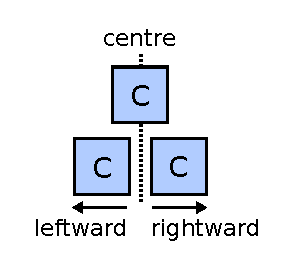
\includegraphics[width=3.5cm]{figures/ch3/c_centre.pdf}
\caption{Schematic illustration of the c-centre effect adapted from \citet{HermesMückeGrice2013}.}
\label{fig:c-centre}
\end{figure}

\medskip\noindent \textit{Code used in this section: coupled\_osc.m}

\subsection{Modelling dynamics of categoriality and continuity}

In the last section, dynamical models of motion and articulation have been presented. Crucially, these models do not only entail mere physical descriptions of the mechanism of speech production but put the dynamical approach they employ in a phonological, cognitive perspective: The gestures of Articulatory phonology are viewed as phonological primitives, the coordination patterns of the coupled oscillators model shape phonological patterns of syllable structure. This perspective maintains that both categorical aspects and continuous aspects of speech can be described jointly by dynamical models. The current section explores this idea more explicitly by presenting some interesting and influential approaches to modelling categoriality and continuity in the sound pattern of language.

\subsubsection{Perceptual categories}

\citet{Tulleretal1994} present a dynamical model that is able to account for interesting results in the perception of speech sound categories. Their work illustrates how the stability of speech sound categories and their perception can be modelled while including flexibility of the perceptual responses.

The authors exposed participants to ordered continua between English \emph{say} and \emph{stay} and between \emph{stay} and \emph{say}. To be more specific, the gap duration between \emph{s} and \emph{ay} increases and then decreases with each stimulus during one experiment run. The participants were tasked to categorise each stimulus in a forced choice task. Two dominant response patterns are evident in the data. In one response pattern, the category switch in the increasing order (the gap duration becomes larger) is later compared to the decreasing order (the gap duration becomes smaller). In other words, for the change from \emph{say} to \emph{stay} a larger gap is necessary than for the change from \emph{stay} to \emph{say}. This response pattern is called \emph{hysteresis}. In the other response pattern, the category switch is earlier in the increasing order compared to the decreasing order. For the change from \emph{say} to \emph{stay} a smaller gap is necessary than for the change from \emph{stay} to \emph{say}. This response pattern is called \emph{enhanced contrast}. Both patterns are illustrated in the two top panels of Figure \ref{fig:tuller_response}. The figure also shows the response pattern \emph{critical boundary} in which the category switch occurs at the same point in the acoustic continuum in both increasing and decreasing order. In the data of \citet{Tulleretal1994}, the response patterns hysteresis and enhanced contrast dominate while the pattern critical boundary is rarely found.

\begin{figure}
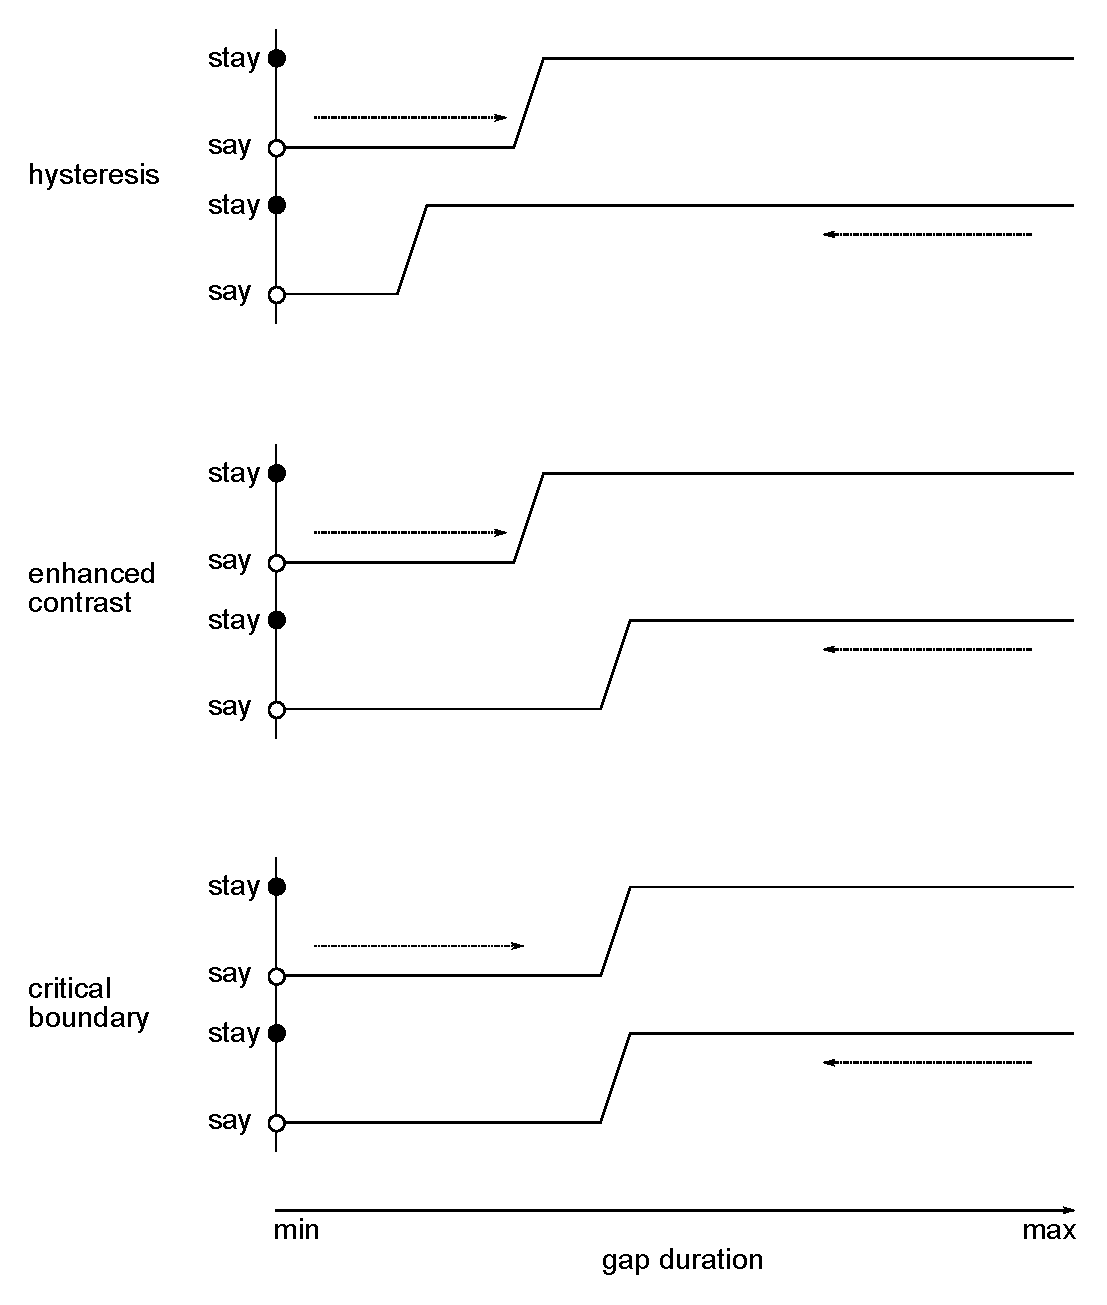
\includegraphics[width=11cm]{figures/ch3/tuller_etal_1994_response_patterns.pdf}
\caption[Possible response patterns of \citet{Tulleretal1994}.]{Possible response pattern of \citet{Tulleretal1994}: hysteresis (top), enhanced contrast (middle), critical boundary (bottom).}
\label{fig:tuller_response}
\end{figure}

\citet{Tulleretal1994} propose a model that is similar to the double well potential introduced in the first part of the chapter in Equation \ref{eq:double_well_potential} and illustrated in Figure \ref{fig:double_well_potential} with a slight difference: The control parameter $k$ occurs with a positive sign in the present model, see Equation \ref{eq:tuller_potential_equation}. The effect of this difference is simply that the scaling of the control parameter has the opposite effect. For positive $k$ values, e.g. $k = 1$, the landscape is tilted to the left, for negative $k$ values, e.g. $k = -1$, it is tilted to the right. 
To connect this attractor landscape to the perceptual data, one attractor is associated with the percept of \emph{say}, the other with \emph{stay}, see Figure \ref{fig:tuller_potential}. While listening to the ordered continuum from \emph{say} to \emph{stay}, the control parameter increases and the attractor landscape gradually tilts to the side of \emph{stay}. When the critical boundary $k_c$ is reached, the \emph{say} attractor is destabilised and the percept changes to \emph{stay}. The process takes place analogously from \emph{stay} to \emph{say} when the control parameter decreases (in this case, the critical boundary is $-k_c$).

\begin{equation}
V(x) = kx - \frac{x^2}{2} + \frac{x^4}{4}
\label{eq:tuller_potential_equation}
\end{equation}

\begin{figure}
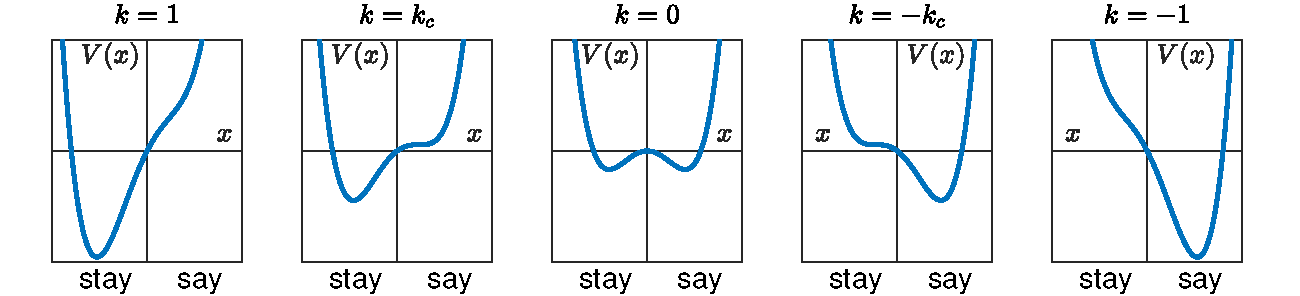
\includegraphics[width=\textwidth]{figures/ch3/tuller_potential.pdf}
\caption{Potential function of \citet{Tulleretal1994} for different values of the control parameter $k$.}
\label{fig:tuller_potential}
\end{figure}

In the response patterns described above, the switch from one category to the other (i.e. \emph{say} to \emph{stay} or \emph{stay} to \emph{say}) is at different points in the continuum. For the model, this means that the critical value of the control parameter $k$ in both sides (towards \emph{stay} or towards \emph{say}) has to occur with different gap durations in the response patterns. To explain this phenomenon, \citet{Tulleretal1994} hypothesise that $k$ depends on a variety of variables and is determined by the function given in Equation \ref{eq:tuller_k_formula}. In this function, $k_0$ is the value of $k$ at the beginning of the run, i.e. $-1$ when the participant starts listening to the continuum with increasing gap durations from \emph{say} to \emph{stay}. $\lambda$ is a variable that is proportional to the gap duration and thus represents the position on the acoustic continuum. $\lambda_f$ is the value of $\lambda$ at the other end of the continuum, i.e. the maximal gap duration when the trial starts with \emph{say} (without a gap). The variable $n$ represents the number of stimuli that the participant already listened to, $n_c$ denotes a critical number of trials defined as 50\% of the trials. $\theta(n-n_c)$ is a step function that is defined as $0$ when $n < n_c$, i.e. in the first half of the trial, and $1$ when $n \geq n_c$, i.e. in the second half of the trial. The variable $\epsilon$ ``represents the lumped effect of learning, linguistic experience, and attentional factors” \citep[8]{Tulleretal1994}. This last parameter is a very important parameter for the model because it plays a major role in explaining the response patterns introduced above.

\begin{equation}
k(\lambda) = k_0 + \lambda + \frac{\epsilon}{2} + \epsilon\theta(n-n_c)(\lambda-\lambda_f)
\label{eq:tuller_k_formula}
\end{equation}

Figure \ref{fig:tuller_colour_map} provides an illustration of the relation between $\epsilon$, gap duration represented by $\lambda$ and the control parameter $k$ as a colour map. The colours represent the values of $k$ determined with the formula of Equation \ref{eq:tuller_k_formula}. The left plot presents the predictions for the first half of the run (increasing gap durations), the right plot presents the predictions for the second half of the run (decreasing gap durations). The colours are only shown for the range of $k$ values in the interval of $[-1, 1]$. Of course $k$ further increases (left plot) or decreases (right plot) through the white area but the restriction to this range makes the colour contrasts stronger and thus visualises the differences better. Both plots show that the colours reflecting the values of the control parameter $k$ are distributed roughly diagonally over the plots. This structure illustrates that for the same gap durations, $k$ values are higher when $\epsilon$ is large in the first half of the run. The opposite is true for the second half of the run where $k$ values are lower when $\epsilon$ is large. 

\begin{figure}
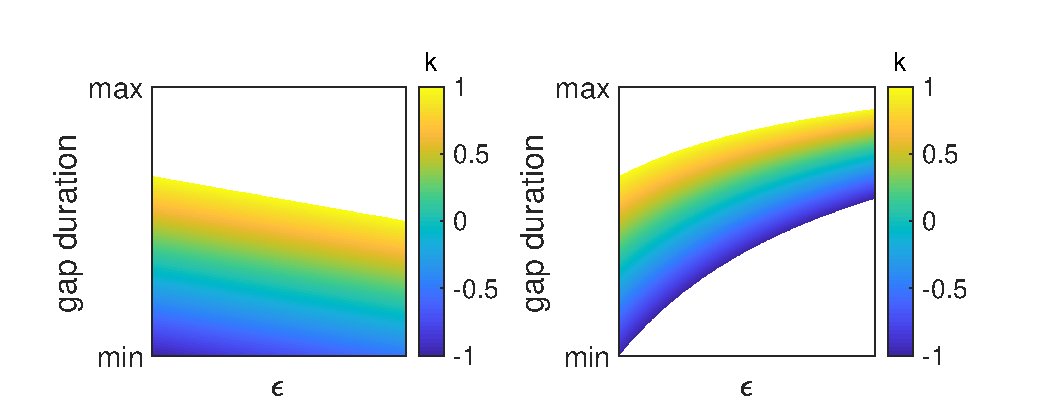
\includegraphics[width=12cm]{figures/ch3/tuller_map.pdf}
\caption[Colour maps representing the values for the control parameter $k$ in relation to $\epsilon$ and gap duration in the \citet{Tulleretal1994} model.]{Colour maps representing the values for the control parameter $k$ in relation to $\epsilon$ and gap duration in the \citet{Tulleretal1994} model. Left: first half of the run with increasing gap durations (small $n$). Right: second half of the run with decreasing gap durations (large $n$).}
\label{fig:tuller_colour_map}
\end{figure}

Recall that the system stays in the attractor as long as the critical value of $k$ that destabilises the attractor is not crossed. When it is crossed, the system moves to the remaining attractor and the percept changes. In a forced choice experiment, the participant changes the response at that point. It is thus sensible to investigate which value of $\lambda$, i.e. which gap durations, yield the critical value of $k$ for different values of $\epsilon$. The thick lines in Figure \ref{fig:tuller_lambda_epsilon} show at which gap duration (y-axis) the critical boundary $k$ occurs as a function of $\epsilon$ (x-axis). The shaded area in the left and middle panel is the span of gap durations for which the system has two attractors, i.e. the control parameter $k$ is between the critical values on both sides $-k_c$ and $k_c$.

The left panel of \ref{fig:tuller_lambda_epsilon} presents the predictions for the first half of the run. The plot is to be read from bottom to top as the arrows indicate, i.e. from no gap to the maximal gap duration (\emph{say} to \emph{stay}). The number of perceived stimuli $n$ is small in this first half and under the threshold  $n_c$ (and thus $\theta(n-n_c) = 0$). When $\epsilon$ is small (left on the x-axis), the categorisation is only dependent on the gap duration. However, for larger $\epsilon$ values, the gap duration needed to shift the percept from \emph{say} to \emph{stay} decreases. In other words, the larger $\epsilon$, the earlier the switch from one category to the other when going from no gap to the maximum gap.

The middle panel of \ref{fig:tuller_lambda_epsilon} shows the predictions for the second half of the run. This plot is to be read from top to bottom, i.e. from the maximal gap duration to no gap (\emph{stay} to \emph{say}). The number of perceived stimuli in the second half is large and above the threshold $n_c$ (and thus $\theta(n-n_c) = 1$). In this case, the model predicts that for larger $\epsilon$ values, the gap duration needed to switch the percept from \emph{stay} to \emph{say} is larger compared to smaller values of $\epsilon$. The larger $\epsilon$, the earlier the switch from from \emph{stay} to \emph{say} when going from the maximum gap to no gap.

The right panel of \ref{fig:tuller_lambda_epsilon} combines the thick lines of the two neighbouring plots. There is a critical value of $\epsilon$, namely $\epsilon_c$, for which the category switch occurs at the same gap duration in both halves of the run. At this point the two lines intersect. When $\epsilon$ is below $\epsilon_c$, the percept changes later and the observed response pattern is \emph{hysteresis}. This is visualised by the line of the first half of the run being positioned above the line of the second half of the run. Going from bottom (no gap) to top (maximum gap) in the first half of the run, the critical boundary of $k$ is reached at a longer gap duration. Going from top (maximum gap) to bottom (no gap) in the second half of the run, the critical boundary of $k$ is reached at a shorter gap duration. 

When $\epsilon$ is above the critical $\epsilon_c$, the percept changes earlier and the observed response pattern is \emph{enhanced contrast}. This is illustrated by the fact that the line of the first half of the run  is positioned under the line of the second half of the run. Going from bottom (no gap) to top (maximum gap) in the first half of the run, the critical boundary of $k$ is reached at a shorter gap duration. Going from top (maximum gap) to bottom (no gap) in the second half of the run, the critical boundary of $k$ is reached at a longer gap duration.

\begin{figure}
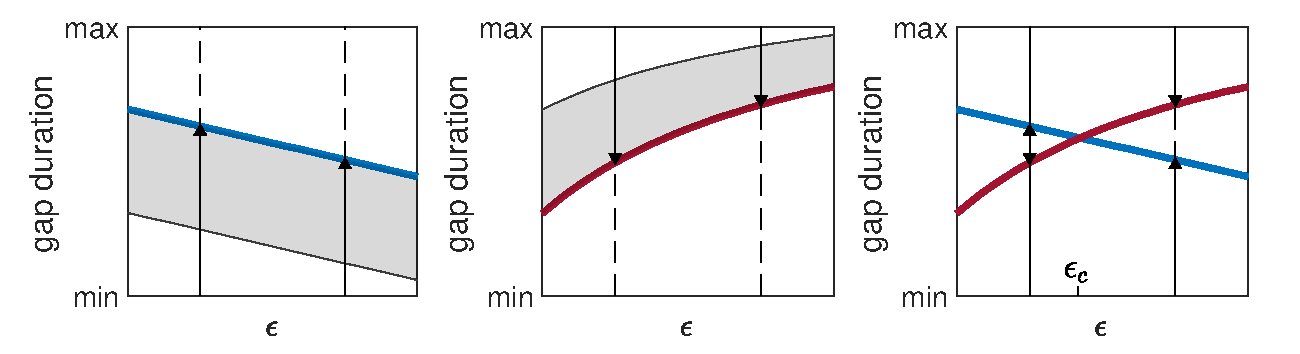
\includegraphics[width=\textwidth]{figures/ch3/tuller_lambda_epsilon_plane.pdf}
\caption[Location of critical values of the control parameter $k$ in the acoustic continuum of gap duration as a function of the parameter $\epsilon$ in the \citet{Tulleretal1994} model.]{Location of critical values of the control parameter $k$ in the acoustic continuum of gap duration as a function of the parameter $\epsilon$ in the \citet{Tulleretal1994} model. Left: first half of the run (increasing gap duration, small $n$). Middle: second half of the run (decreasing gap duration, large $n$). Right: superposition of critical boundary in first and second run.}
\label{fig:tuller_lambda_epsilon}
\end{figure}

The model of \citet{Tulleretal1994} shows how the flexibility and context dependency of perceptual categories can be modelled using the double well potential with two attractors presented earlier in this chapter. The next section will present work adapting a similar potential for the modelling approach to capture continuous and categorical variation found in production data.

\medskip\noindent \textit{Code used in this section:\\
tuller\_1994\_potential.m, tuller\_1994\_crit\_lambda.m, tuller\_1994\_map.m}

\subsubsection{Incomplete neutralisation}

As introduced in the previous chapter, the phenomenon of incomplete neutralisation of syllable final obstruents in German poses a major problems for purely symbolic approaches to phonology and a modular separation of phonetics from phonology. To remind the reader, a large body of work has centred around the question whether the voicing contrast of obstruents in syllable coda positions in German is complete or not. Numerous studies have shown that there are indeed differences between the final obstruents of words like \emph{Rat} and \emph{Rad} such that the acoustic features of the devoiced final obstruent [t] in \emph{Rad} are modulated subtly in the direction of the voiced [d].

In addition, a study by \citet{PortCrawford1989} suggests that the communicative context modulates the differences between the obstruents. When the speaker produces the words containing the obstruents in direct contrast (``Ich habe Rad gesagt, nicht Rat") and a listener is tasked to write down the correct word, the supposedly neutralised obstruent shifts more in the direction of the voiced variant compared to a task in which the speaker simply reads the words in a list.

\citet{GafosBenus2006} propose a dynamical model that is able to capture the differences between the obstruents in relation of the speaker's intent to maintain the contrast. In this model, the categorical nature of the phonological voicing contrast can be maintained while allowing for fine-grained differences. In the first part of the model, the intention of a speaker to produce a voiced or a voiceless obstruent is described by defining one attractor for each voicing value on a continuum of voicing. The continuum of voicing are all possible states $x$ of the systems. The intention to produce a contrast is formally modelled with the force function $F(x)$ in Equation \ref{eq:gafos_benus_intentional_force_potential}, where $x_{req}$ is the \emph{required} (i.e. intended) value on the voicing continuum $x$. Crucially, $x_{req}$ is the location of the attractor of this system. For the voiceless obstruent, a location in the positive range of $x$ denoted by $x_0$ is chosen. For the voiced obstruent, a location the negative range of $x$ denoted by $-x_0$ is chosen. The exact values do not play a role in the modelling approach, it is only important that they are distributed on both sides of zero.

The second line of Equation \ref{eq:gafos_benus_intentional_force_potential} presents the potential energy function $V_F(x)$ that is obtained by integration of the negative of the force function. Figure \ref{fig:gafos_benus_intentional_force_potential} displays $F(x)$ and $V_F(x)$ with $x_{req} = -x_0$ on the left and $x_{req} = x_0$ on the right. The control parameter of this system is $\theta$, a quantity representing the intent of the speaker to produce this value of voicing $x_{req}$. In the further description of the model, the role of the parameter $\theta$ will become clearer.

\begin{equation}
\begin{split}
F(x) = \theta (x_{req} - x) \\
V_F(x) = \theta \frac{x^2}{2} -\theta x_{req} x
\end{split}
\label{eq:gafos_benus_intentional_force_potential}
\end{equation}

\begin{figure}
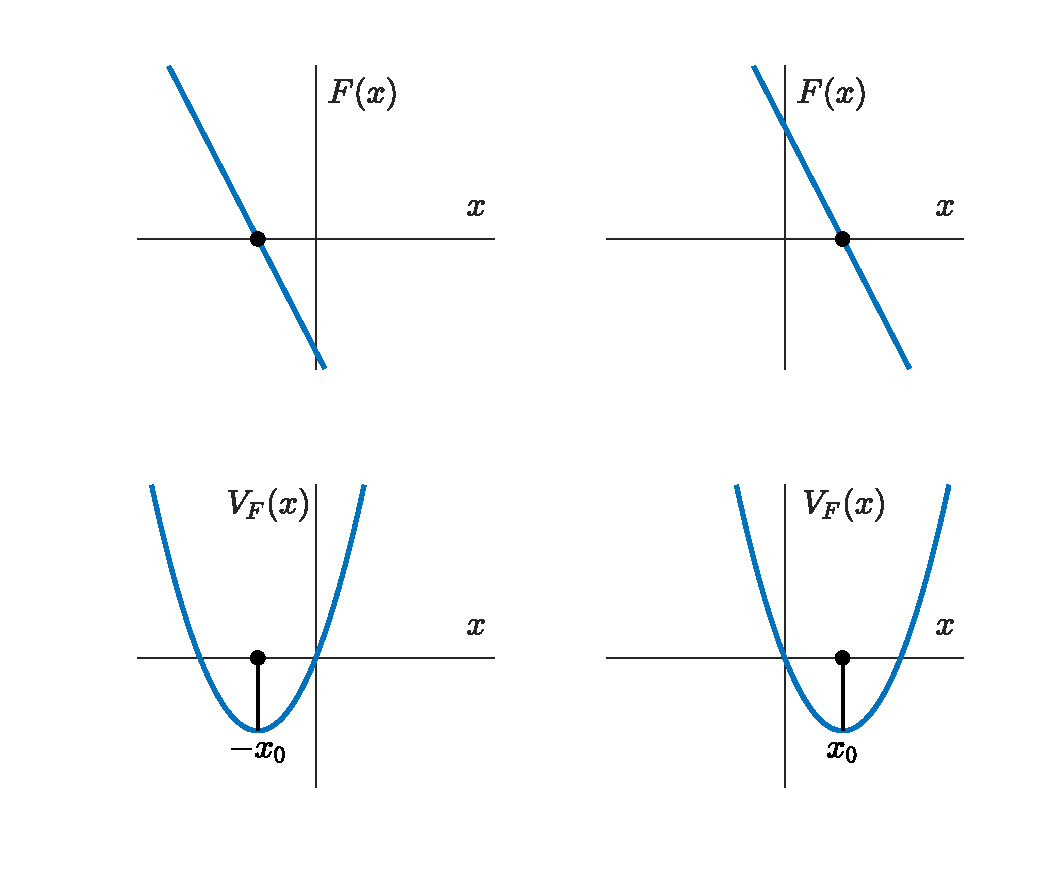
\includegraphics[width=10cm]{figures/ch3/gafos_benus_intentional_dynamics.pdf}
\caption[Force and potential for voiced and voiceless obstruents in the \citet{GafosBenus2006} model.]{Force (top) and potentials (bottom) for $x_{req} = -x_0$ (voiced) and $x_{req} = x_0$ (voiceless) in the \citet{GafosBenus2006} model. Vertical lines in the potential visualise the location of the minimum at the value of $x_{req}$ ($-x_0$ or $x_0$).}
\label{fig:gafos_benus_intentional_force_potential}
\end{figure}

In the second part of the model, an additional force is introduced to account for the fact that German allows for voiceless obstruents only in syllable coda. Here, the same attractor landscape is used as in \citet{Tulleretal1994}, its force $M(x)$ and potential $V_M(x)$ are given in Equation \ref{eq:gafos_benus_coda_force_potential}. For the control parameter $k$, a value beyond the critical threshold of $-k_c$ is chosen ($-1$ in the illustration) such that the landscape is tilted to the voiceless side and the voiceless attractor is the only attractor that remains, see Figure \ref{fig:gafos_benus_coda_potential}. The presence of only on attractor reflects the fact that there is one possibility for obstruents in syllable codas: voiceless.

\begin{equation}
\begin{split}
M(x) = -k+x-x^3\\
V_M(x) = kx - \frac{x^2}{2} + \frac{x^4}{4}
\end{split}
\label{eq:gafos_benus_coda_force_potential}
\end{equation}

\begin{figure}
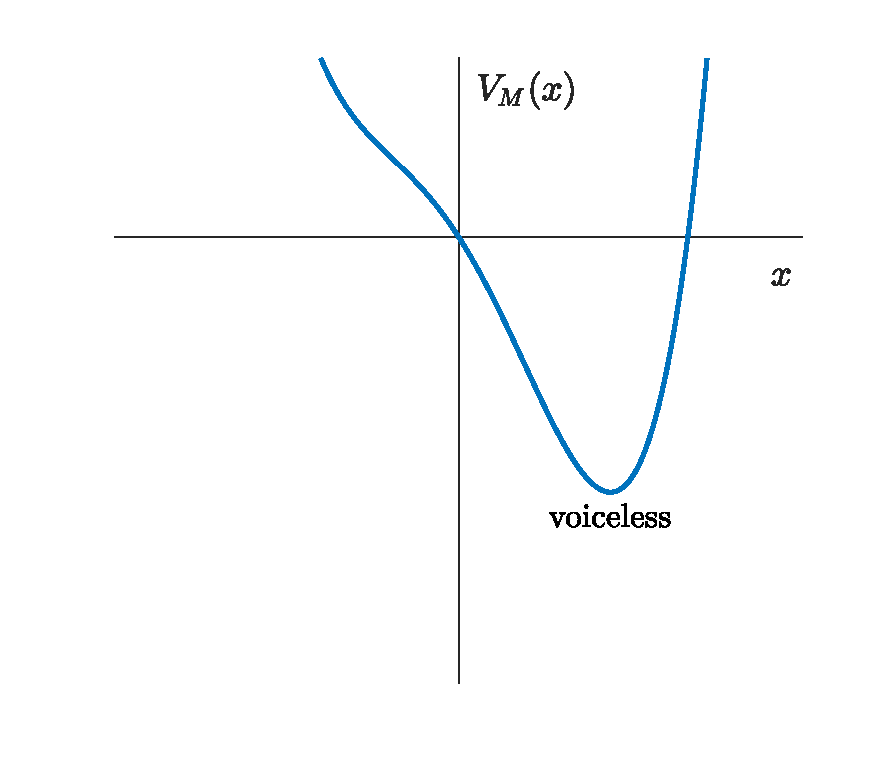
\includegraphics[width=8cm]{figures/ch3/gafos_benus_coda_potential.pdf}
\caption[Tilted double well potential $V_M(x)$ of the \citet{GafosBenus2006} model.]{Double well potential $V_M(x)$ of the \citet{GafosBenus2006} model tilted to the right side to represent the fact that only the voiceless attractor is available in coda position.}
\label{fig:gafos_benus_coda_potential}
\end{figure}

\citet{GafosBenus2006} draw parallels of their dynamical model to an analysis of the phenomenon in optimality theory (OT), a purely symbolic framework. In such an analysis, the presence of one attractor for voiced and one attractor for voiceless obstruents as in the first part of the model corresponds to a \emph{faithfulness} constraint. This constraint is violated when the output form deviates from the underlying representation, see Chapter \ref{chapter_pandp}. In other words, the constraint entails that it is the intention of the speaker to produce outputs as close as possible to the underlying representation. The second part of the model in which only an attractor for voiceless is present corresponds to a \emph{markedness} constraint that requires coda consonants to be voiceless in German.

The interaction of the two parts of the model is achieved by adding up the two forces $F(x)$ and $M(x)$ to obtain the final force function of the system (see Equation \ref{eq:gafos_benus_interaction} for the combined force and potential). In an OT analysis, the markedness constraint would be ranked higher than the faithfulness constraint eliminating any influence of the latter. In the interaction of the present model, however, the force $F(x)$ can influence the outcome of the whole system even if the force $M(x)$ might be stronger. This means that despite the pressure to realise only voiceless obstruents in syllable-final position, the ``underlying" voicing can still have an impact. The size of this impact can be scaled by virtue of a scalar value.

\begin{equation}
\begin{split}
M(x) + F(x) = -k+x-x^3 + \theta (x_{req} - x) \\
V_M(x) + V_F(x) = V(x) = kx - \frac{x^2}{2} + \frac{x^4}{4} + \theta \frac{x^2}{2} - \theta x_{req} x
\end{split}
\label{eq:gafos_benus_interaction}
\end{equation}

The resulting patterns are illustrated in Figure \ref{fig:gafos_benus_combined_potentials}. The top panel presents the outcomes for the underlying voiced obstruent, i.e. $x_{req} = -x_0$, for three possible values of $\theta$: 0.1, 0.3, and 0.5. With increasing $\theta$ the attractor basin drifts subtly towards the negative, voiced part of the continuum $x$ while it stays in the general region of the positive, voiceless part of $x$. As a result, the voiceless obstruent becomes \emph{slighty more voiced}. The production of words like \emph{Rat} with underlyingly voiceless obstruent, i.e. $x_{req} = x_0$, does not lead to the same conflict. The lower panel of Figure \ref{fig:gafos_benus_combined_potentials} shows for the same three values of $\theta$ that the location of the attractor does not change. 

To summarise, producing the intended obstruent and adhering to voiceless obstruents in codas leads to a conflict in words like \emph{Rad}. While this conflict is resolved by a constrain ranking and a single resulting outcome in OT, the interaction can be modulated continuously in the model of \citet{GafosBenus2006}. The effect of $F(x)$ on $M(x)$ is a ``pull" towards more voiced productions on the voicing continuum $x$. This ``pull" is modulated by the scaling of the control parameter $\theta$. 

\begin{figure}
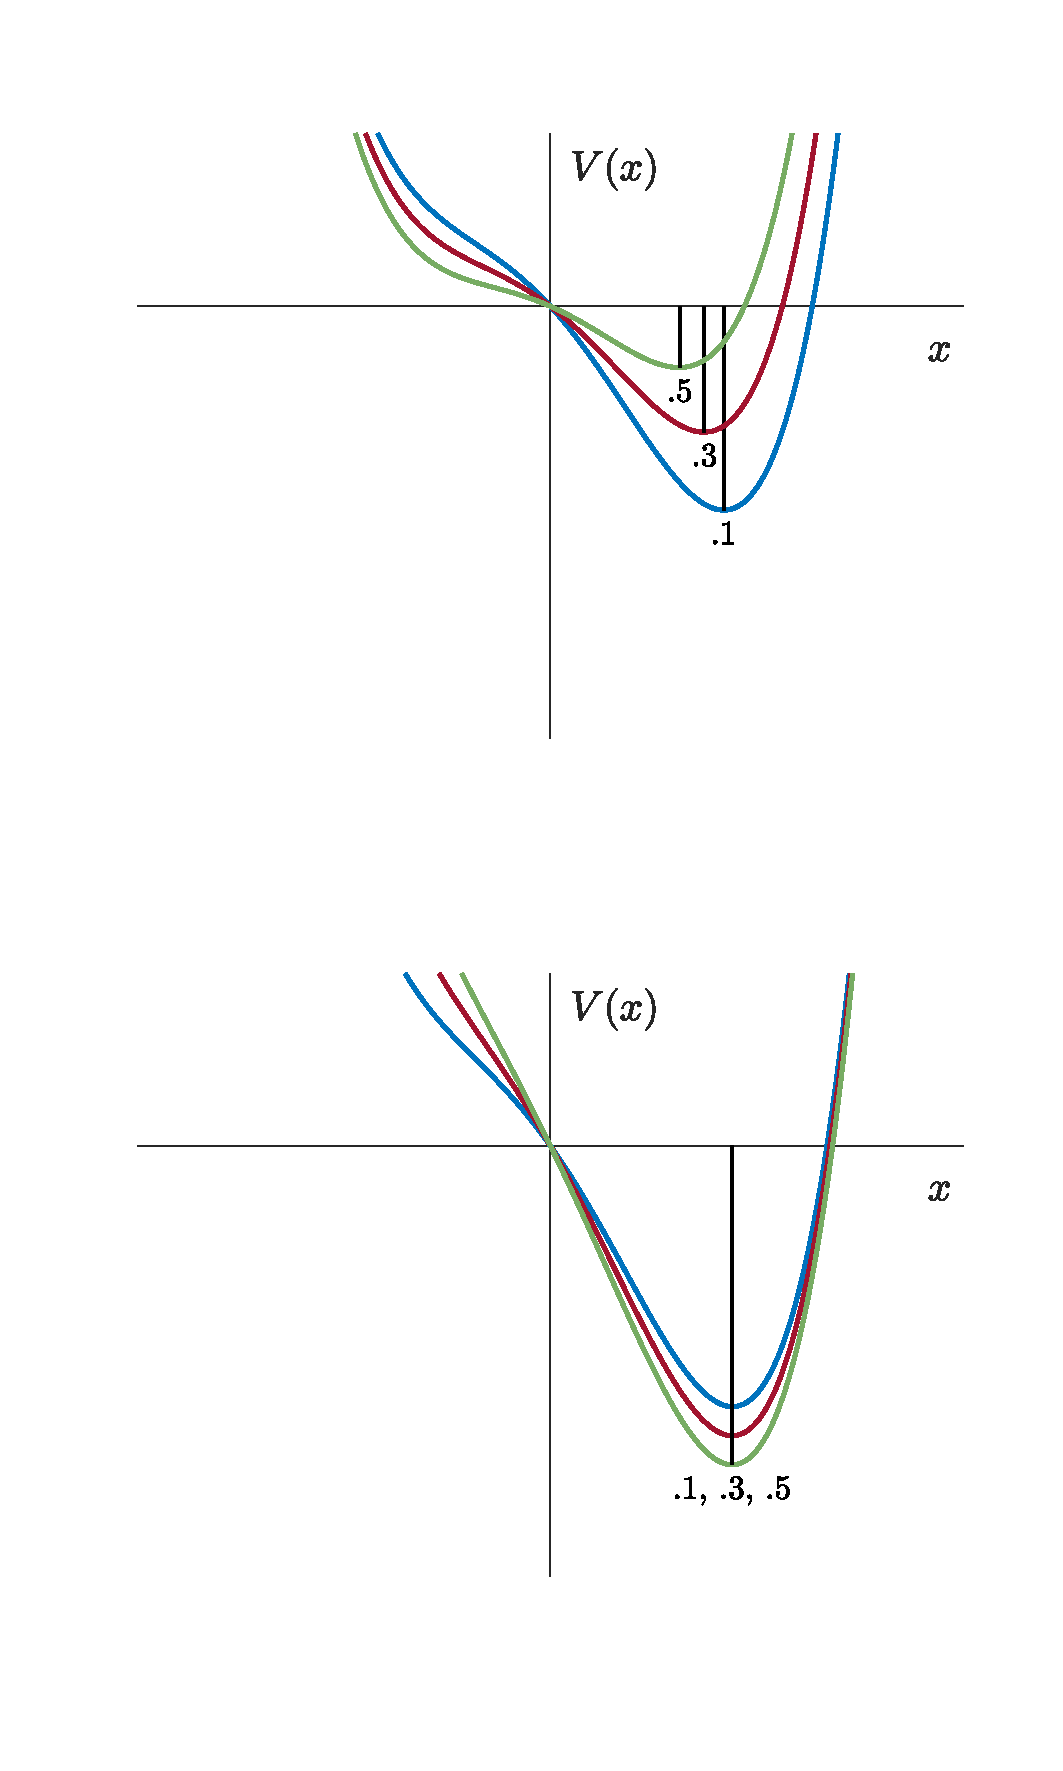
\includegraphics[width=8.5cm]{figures/ch3/gafos_combined_potentials.pdf}
\caption[Combined potentials of the model of \citet{GafosBenus2006}.]{Combined potentials of the model of \citet{GafosBenus2006} for three values of the control parameter $\theta$. Vertical lines indicate the location of the attractor. Blue: $\theta = 0.1$, red: $\theta = 0.3$, green: $\theta = 0.5$. $k$ is constant at $-1$ in all graphs.}
\label{fig:gafos_benus_combined_potentials}
\end{figure}

\medskip\noindent \textit{Code used in this section: gafos\_benus\_incomplete\_neutralisation.m}

\subsubsection{Transparent vowels}

In the previous chapter, the phenomenon of transparent vowels in Hungarian has been introduced. It was explained there that the front unrounded vowels function as transparent vowels as they can occur between the vowel triggering the vowel harmony and the target of the vowel harmony but have been described as not affecting the process of vowel harmony. For example, the back vowel /aː/ of the stem \emph{kávé} /kaːveː/ (`coffee') determines the vowel /ɔ/ of the suffix \emph{nak} /nɔk/ regardless of the intervening unrounded front vowel in the stem. 

The supposedly insignificant role of the transparent vowels in the determination of suffixes, however, is questioned by observations of the behaviour of transparent vowels. Stems that only have transparent vowels can trigger both front and back suffixes \citep{Vago1980, GafosBenus2006} although the distribution of the suffixes is not even, as the majority of stems triggers front suffixes \citep{HayesLonde2006, GafosBenus2006}. In addition, the probability of selecting a back suffix decreases with increasing numbers of transparent vowels intervening between a back stem vowel and the suffix \citep{GafosBenus2006}.

\citet{GafosBenus2006} (as well as \citealp{Benus2005}) hypothesise that systematic articulatory differences in transparent vowels are responsible for the suffix choice. In consequence, transparent vowels may participate in the process of vowel harmony. The authors report data from a study employing electromagnetic articulography and ultrasound to track the position of the tongue and investigate the tongue shape. They show that the tongue is more advanced when articulating transparent vowels in stems that trigger front suffixes compared to transparent vowels in stems that trigger back suffixes. A dynamical model is proposed that resembles the model for incomplete neutralisation outlined in the previous section although the two deal with rather different phonological phenomena. Nevertheless -- like the model for incomplete neutralisation -- the present model links \emph{continuous} and \emph{categorical} aspects in one formal approach.

The first part of the model is a formalisation of articulatory gestures by point-attractor dynamics which is in line with the description of gestures in Articulatory phonology (see also the damped harmonic oscillator presented above). The dynamics of the spatial dimension of constriction location of the tongue body is modelled with a monostable potential as given in its general form in the first line of Equation \ref{eq:gafos_benus_constriction_location}. $x_0$ represents the target constriction location. The factor $\gamma$ represents the strength with which this gesture controls the articulator, the consequence of its scaling will become clearer in the further description. The equation also presents two potentials in the second and third line, one for back vowels and one for front vowels. The factor $\gamma$ is now called $\alpha$ for back vowels and $\beta$ for front vowels. For the back vowel, $x_0$ is chosen as $-2$; for the front vowel, $x_0$ is chosen as $2$. The two potentials $V_B(x)$ (back vowels) and $V_F(x)$ (front vowels) are shown in Figure \ref{fig:gafos_benus_constriction_location_potentials} (with $\alpha = \beta = 1$). 

\begin{equation}
\begin{split}
V(x) = \gamma (x-x_0)^2 \\
V_B(x) = \alpha (x+2)^2 \\
V_F(x) = \beta (x-2)^2
\end{split}
\label{eq:gafos_benus_constriction_location}
\end{equation}

\begin{figure}
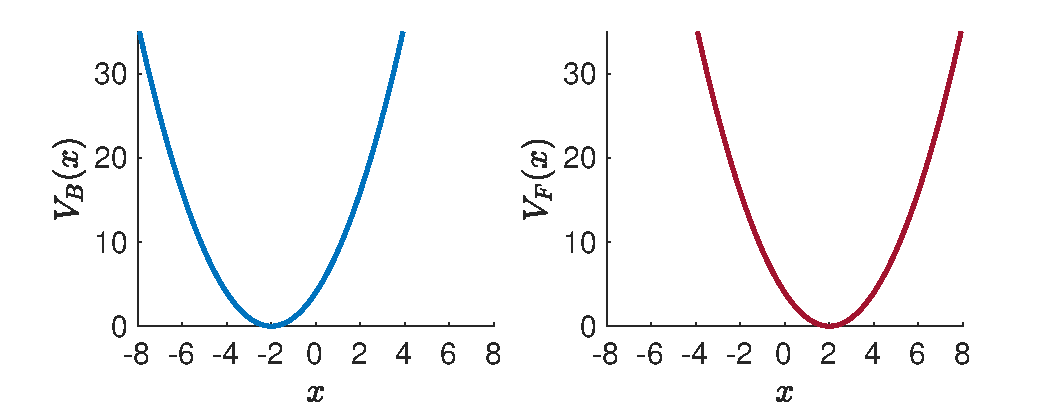
\includegraphics[width=11cm]{figures/ch3/gafos_benus_constriction_location_potential.pdf}
\caption[Monostable potentials modelling the tongue body gesture with regard to constriction location.]{Monostable potentials modelling the tongue body gesture with regard to constriction location. Left: $V_B(x)$ for back vowels, right: $V_F(x)$ for front vowels.}
\label{fig:gafos_benus_constriction_location_potentials}
\end{figure}

The effect of coarticulation of vowels can be modelled as gestural blending by assuming linear combinations of the respective vowel potentials, $V_B(x) + V_F(x)$, and adjusting the values for the factors $\alpha$ and $\beta$. Simply speaking: The factors $\alpha$ and $\beta$ represent weights that specify which gesture will have a dominant effect in the blending. In this way, the influence of a preceding vowel on the target constriction location of a vowel can be captured. Figure \ref{fig:gafos_benus_blending_examples} illustrates two examples for combined potentials produced by linear combinations of the vowel potentials for different values of $\alpha$ and $\beta$. In this figure, the solid lines represent the two potentials for back and front vowels $V_B(x)$ and $V_F(x)$ as in the previous figure. The dotted line shows the graph of the combined potential: $V_B(x) + V_F(x)$. The position of the minimum of this graph on the $x$ axis indicates the vowel target that results from the blending. In the left panel, the case $\alpha = \beta = 1$ is shown, the hypothetical vowel has a target midway between the front and the back vowel. The experimental data of \citet{GafosBenus2006} showed that the retraction of the front vowel is only subtle. Therefore, the right panel shows an example where the weight of the back vowel, $\beta$, is smaller than the weight of the front vowel, $\alpha$: $\alpha = 1, \beta = 3$. The outcome is a vowel that has a constriction location target slightly lower than the original front vowel modelled by $V_F(x)$. 

\begin{figure}
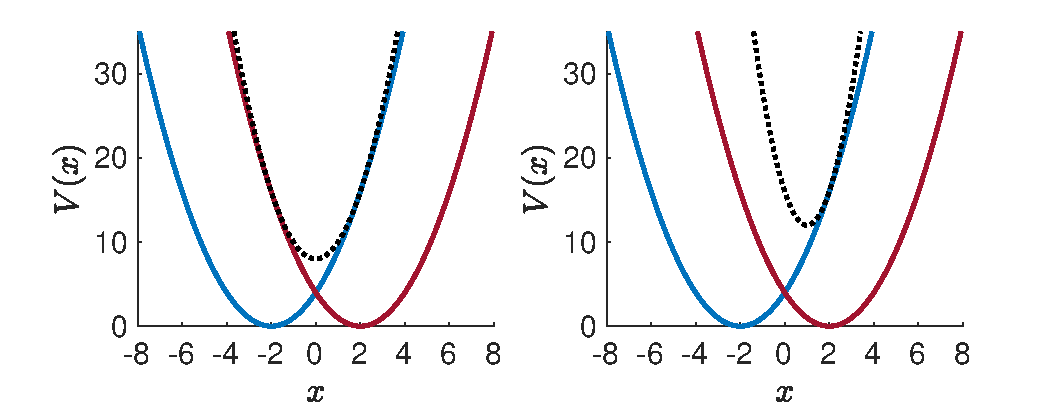
\includegraphics[width=11cm]{figures/ch3/gafos_benus_blending_examples.pdf}
\caption[Examples for blending of vowel gestures by linear combination of the potentials corresponding to each vowel in the model of \citet{GafosBenus2006}.]{Examples for blending of vowel gestures by linear combination of the potentials corresponding to each vowel. Solid lines: individual vowel potentials (blue for $V_B(x)$ and red for $V_F(x)$). Dotted line: combined potential $V_B(x) + V_F(x)$. The two panels show cases for different weightings of the potentials. Left: $\alpha = \beta = 1$, right: $\alpha = 1, \beta = 3$.}
\label{fig:gafos_benus_blending_examples}
\end{figure}

The degree of retraction of a front vowel is assessed by the quantity $R$ in this model of vowel gesture blending. In the example in the right panel of Figure \ref{fig:gafos_benus_blending_examples}, the front vowel described through the potential $V_F(x)$ has a target constriction location of $2$, the vowel resulting from blending has a target location of $1$. In this case, $R$, representing the difference between the basic front vowel and the vowel retracted by influence of the back vowel, is $1$.

The choice of a front vowel or back vowel suffix can now be modelled employing a dynamical system with a double-well potential that uses the retraction degree $R$ as a control parameter. In the system, one attractor is associated with the back suffix, the other attractor is associated with the front suffix. Hence, the second part of the vowel harmony model of \citet{GafosBenus2006} is given by the force $F(x)$ and potential $P(x)$ in Equation \ref{eq:gafos_benus_vowel_harmony_force_potential}. These equations are similar to those in the previous sections. Note, however, that the exposition deviates slightly here and integrates the coefficients for the quartic term $x^4$ and the linear term $x$ from \citet[][262, footnote 85]{Benus2005}.\footnote{The graphs of \citet{GafosBenus2006} are also based on the coefficient $0.1$ for $x^4$, the coefficient of the linear term $x$ is simply put differently.} The choice of this coefficient does not change the general quality of the model; it merely locates the attractor in regions around $-2$ and $2$ corresponding to the assumed values for front and back constriction locations.

\begin{equation}
\begin{split}
F(x) = (2-3R) - 0.4 x^3 + x\\
P(x) = -(2-3R)x + 0.1 x^4 - 0.5 x^2
\end{split}
\label{eq:gafos_benus_vowel_harmony_force_potential}
\end{equation}

Figure \ref{fig:gafos_benus_suffix_potential} presents the graph of the potential $P(x)$ for different values of the control parameter $R$. If the degree of retraction of the transparent vowel is high, e.g. $R = 1.2$ or $R = 1.0$, the attractor landscape only predicts one possibility for the choice of the suffix: back. The reverse is true when the retraction is small, e.g. $R = 0.2$ or $R = 0.4$, for which only front suffixes are possible. In between these values, the attractor landscape becomes bistable. In this region of intermediate $R$ values, the suffix choice can vary between front and back due to random fluctuations and the initial state.

\begin{figure}
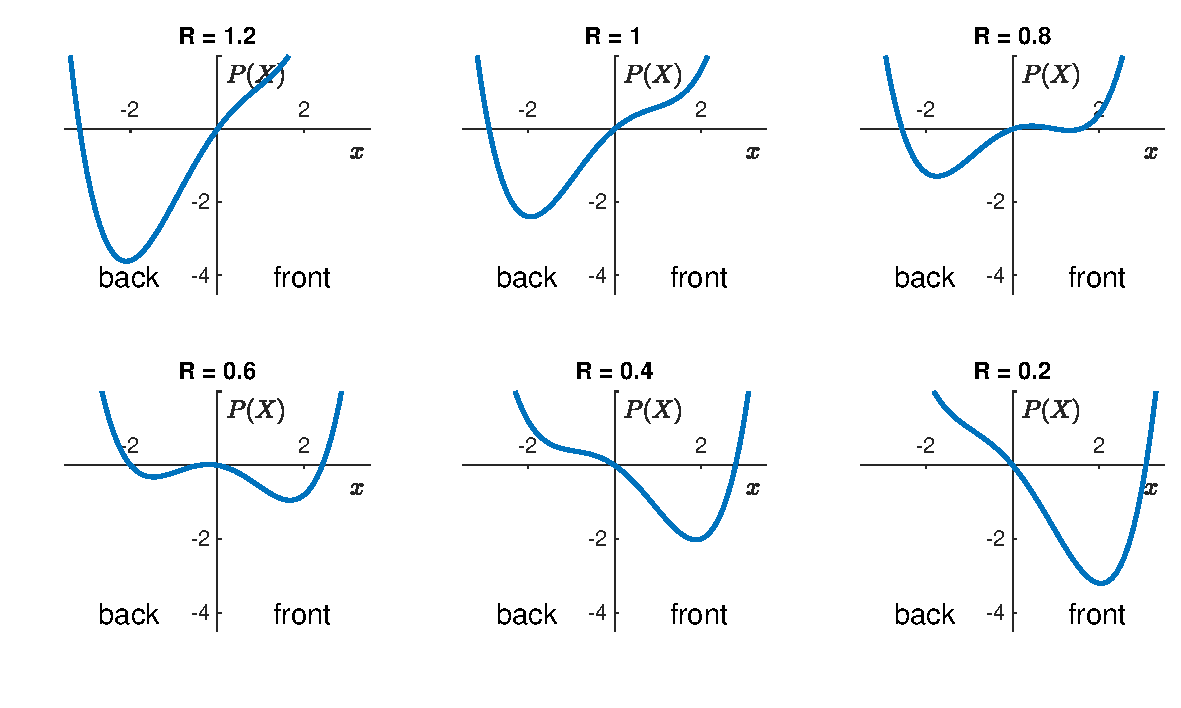
\includegraphics[width=\textwidth]{figures/ch3/gafos_benus_suffix_potential.pdf}
\caption{Suffix choice potential $P(x)$ for different values of the control parameter $R$.}
\label{fig:gafos_benus_suffix_potential}
\end{figure}

The graphs of the potential $P(x)$ shown in Figure \ref{fig:gafos_benus_suffix_potential} illustrate how the scaling of a continuous parameter can lead to categorical changes. Depending on the magnitude of the adjustment of the continuous parameter, only one category remains as the possible output of the system or the system is in principle able to produce two different outcomes. When the system is conceptualised as a stochastic dynamical system, the outcomes of the system depending on the control parameter can be described as statistical distributions. A stochastic system is obtained by the introduction of random fluctuations or noise \citep{Haken1977}, denoted by $\xi_t$ in Equation \ref{eq:gafos_benus_stochastic_system}. $\xi_t$ is conceptualised here as Gaussian white noise with a scaling factor $q$ that determines the strength of the noise \citep{GafosBenus2006}. These statistical distributions of the system's outcome are modulated as a result of the relative stabilities of the attractors. In other words, in the region of bistability, a deeper attractor in the potential is more resistant to random fluctuations than a shallower attractor, it takes more noise to move the system out of the attractor basin. The system is thus more likely to end up in this deeper, more stable attractor.

\begin{equation}
\begin{split}
\dot{x} = F(x) + \text{Noise} = \frac{-dV(x)}{dx} + \xi_t\\
\end{split}
\label{eq:gafos_benus_stochastic_system}
\end{equation}

A description of the distributional patterns of a stochastic system can be obtained in two ways: either analytically by finding a stationary solution to the \emph{Fokker-Planck} equation \citep{Haken1977, FreidlinWentzell1984} or by computational simulation of the system with noise \citep{GafosBenus2006}. The solution to the Fokker-Planck equation is used to compute a probability density distribution. Figure \ref{fig:gafos_benus_probabilities} presents probability distributions obtained in this way for the potential $P(x)$ and the same $R$ values as in Figure \ref{fig:gafos_benus_suffix_potential}.

\begin{figure}
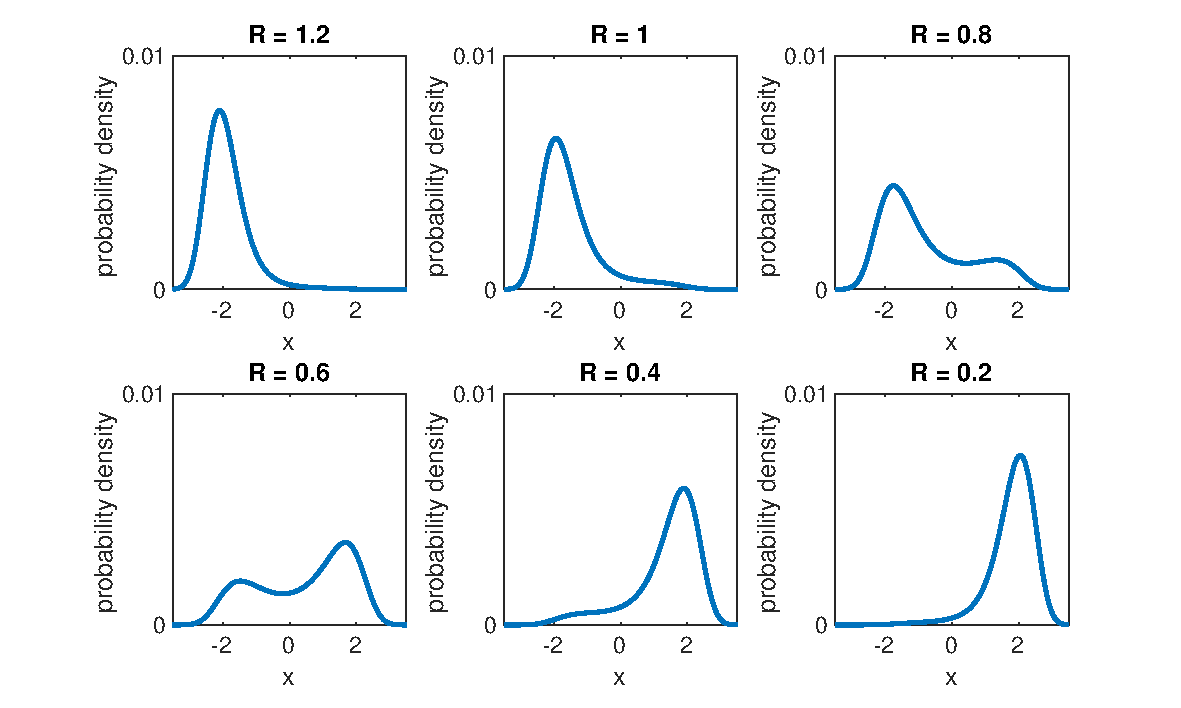
\includegraphics[width=\textwidth]{figures/ch3/gafos_benus_probabilities.pdf}
\caption{Probability density distributions corresponding to the stochastic version of the system described by the potential $P(x)$ for different values of the control parameter $R$.}
\label{fig:gafos_benus_probabilities}
\end{figure}

The simulation of the stochastic system can be carried out by solving the differential equation as described above in Section \ref{sec:diff_equations}. During each time step, noise from a Gaussian distribution is added. After a fixed number of steps, the simulation is finished and the solution is recorded. This procedure is repeated for a number of times in order to obtain a distribution of final solutions. For the solutions shown in the histograms of Figure \ref{fig:gafos_benus_simulation}, the simulation was run for 5000 time steps and repeated to obtain 5000 solutions.\footnote{The simulation is based on the code accompanying \citet{Gafos2006}.} Again, the same values for $R$ as before are chosen in these plots. The outcome of the simulation reproduces the probability density functions shown in the previous figure.

\begin{figure}
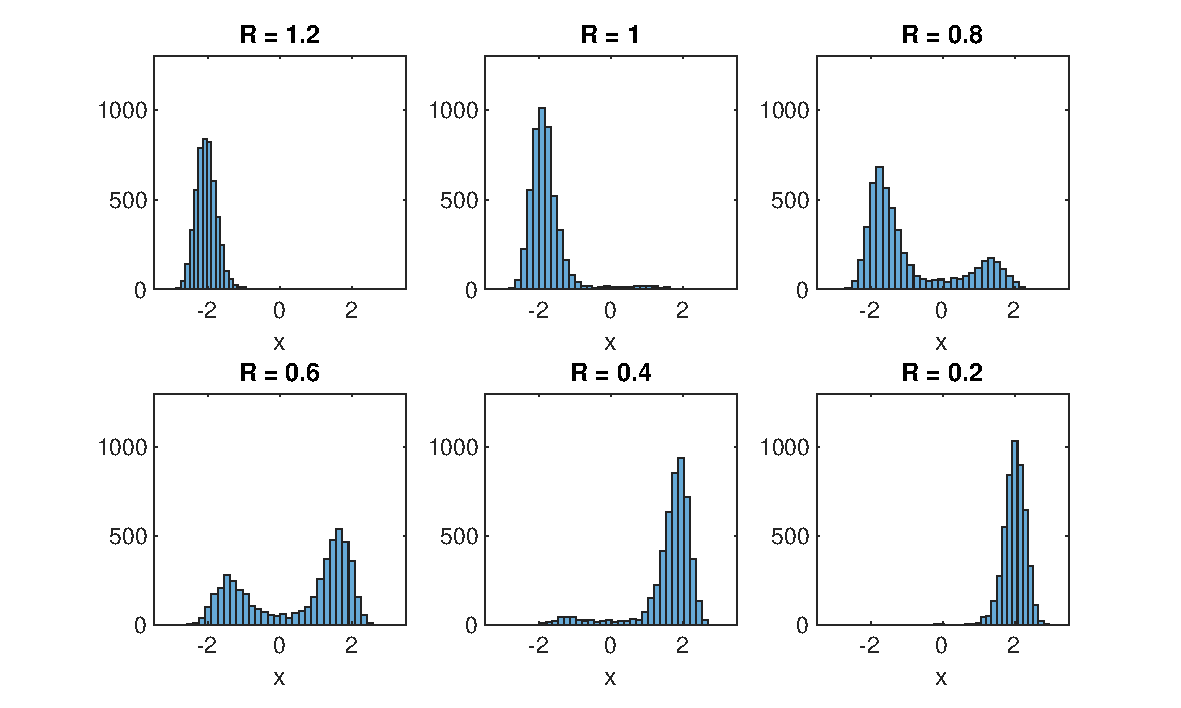
\includegraphics[width=\textwidth]{figures/ch3/gafos_benus_simulation.pdf}
\caption{Simulation results for different values of the control parameter $R$ in the system given by the potential $P(x)$.}
\label{fig:gafos_benus_simulation}
\end{figure}

The concept of the stochastic dynamical system plays a major role for the modelling approach presented in the second part of this book. It makes it possible to leverage the differences in stability of the attractors when multiple attractors are present. This section is completed by taking up the metaphor of a ball rolling in the attractor landscape and adding the notion of noise or random fluctuations to it. Imagine that the ball's trajectory is perturbed by tiny strokes. Sometimes these strokes are stronger, sometimes they are weaker. It fits our intuition well that it takes a stronger stroke to push the ball out of an attractor basin if it is deeper, i.e. more stable, compared to a shallower attractor basin.

\medskip\noindent \textit{Code used in this section: gafos\_benus\_vowel\_harmony.m}

\section{Summary}
This chapter has presented an overview on dynamical systems and their application in the science of language and speech. It has touched upon the fundamental concepts of attractors and multi-stability, and outlined how dynamical systems can be used together with simulation techniques to investigate their predictions in more detail. The most important point to take away from this chapter is that dynamical systems have proven to be suited in reconciling categorical and continuous phenomena in an integrated view and thus provide a toolbox to gain insights into the relation of phonetics and phonology.
  
%\chapter{Prosody, prosodic prominence and focus}
\label{chapter_prosody}

Prosody denotes all aspects of the rhythmical and tonal organisation of spoken communication \citep{Calhoun2007}. Every utterance in every language has prosodic properties \citep{Grice2006}. Languages employ prosody to chunk the stream of speech and to single out certain elements in this stream, like words or syllables. Both mechanisms lend rhythmical and tonal structure to speech. The use of prosodic aspects to single out certain elements has been termed \emph{prosodic prominence}. Prosodic prominence is understood as a relative property as one element is made \emph{prominent} in comparison to other elements \citep{WagnerWatson2010}. Making a word or a syllable in a word more prominent often reflects the speaker's intention to highlight importance or newness of the word or referent denoted by that word in the discourse. Prominence and its relation to discourse play a major role in this work but the demarcating aspects and the marking of edges of prosodic constituents are also discussed to some extent in this chapter.

Among the physical parameters that have attracted most attention in the analysis of prosodic patterns are fundamental frequency (F0), intensity or amplitude, and duration \citep{Ladd2008, Grice2006}. Their perceptual counterparts are pitch, loudness and length. These parameters form a conglomerate of prosodic cues and neither of them is used exclusively for a certain function of prosody. They all play a role in both chunking as well as prominence. F0 movements on or close to a syllable as well as an increase in amplitude and duration can make this syllable stand out from neighbouring syllables. But an F0 movement and an increase in duration are also often used to mark the end of a phrase. In addition, spectral properties of vowels and consonants have been reported to be affected by prosody \citep{Cho2011, Gussenhoven2004}. For example, lending prosodic prominence to a syllable can affect the formant values of the vowel in that syllable. Vowels in more prominent positions tend to be less centralised compared to their counterparts in less prominent positions, revealing a more distinct articulation \citep{DeJong1995, Cho2005, Mücke2018}.

Decades of prosody research have emphasised that prosody has decomposable structure and that the relations of the elements within that structure are important to understand prosody \citep{Ladd2008, Arvaniti2011}. The next section sheds light on prosodic structure (Section \ref{sec:prosodic_structure}). Section \ref{sec:focus1} then takes to a first look at one of the most important functions of prosody in West-Germanic languages, namely the marking of \emph{focus}, and uses the knowledge of prosodic structure to explain the relation of focus and prosody. Section \ref{sec:prosody_catcont} investigates the categorical and continuous aspects of prosody and argues that prosody is characterised by both. In the light of this argumentation, Section \ref{sec:focus2} takes a second look at focus marking and shows that categorical and continuous aspects of prosody are involved in this function of prosody. Section \ref{sec:prosodic_strengthening} gives an overview on how prosody affects movements of supra-laryngeal articulation and points out a strong connection of prosodic structure and what has been described as segmental. Section \ref{sec:focus3} takes a third look at focus beyond tonal properties presenting evidence that prosodic strengthening plays an important role here as well. Section \ref{sec:summary_prosody} summarises the chapter.

\section{Prosodic structure}
\label{sec:prosodic_structure}

A very influential framework for the analysis of prosody is the auto-segmental model \citep{Pierrehumbert1980, Ladd2008}, henceforth abbreviated as AM. This framework stresses the idea that prosodic structure is organised hierarchically and that the tune of an utterance, the \emph{intonation contour}, can be decomposed into smaller units (tones) that are to some extent independent of the words they are produced on. Different hierarchies of prosodic structure have been proposed in the literature \citep{NesporVogel1986, PierrehumbertBeckman1988, Hayes1989, Selkirk1996, ShattuckHufnagelTurk1996}. All proposals share the assumption that utterances can be decomposed into hierarchically organised constituents although they disagree as to the existence of some levels. Most researchers in the field agree upon a minimal structure that can be outlined as follows \citep{Grice2006}: An utterance consists of one or more intonational phrases which contain one or more smaller phrases. Here, an intermediate phrase is assumed as the level between the intonational phrase and the word. A constituent on the smallest level of phrasing contains one or more words, a word contains one or more feet, and a foot contains one or more syllables. This prosodic hierarchy is illustrated with an example in Figure \ref{fig:prosodic_hierarchy}.

\begin{figure}
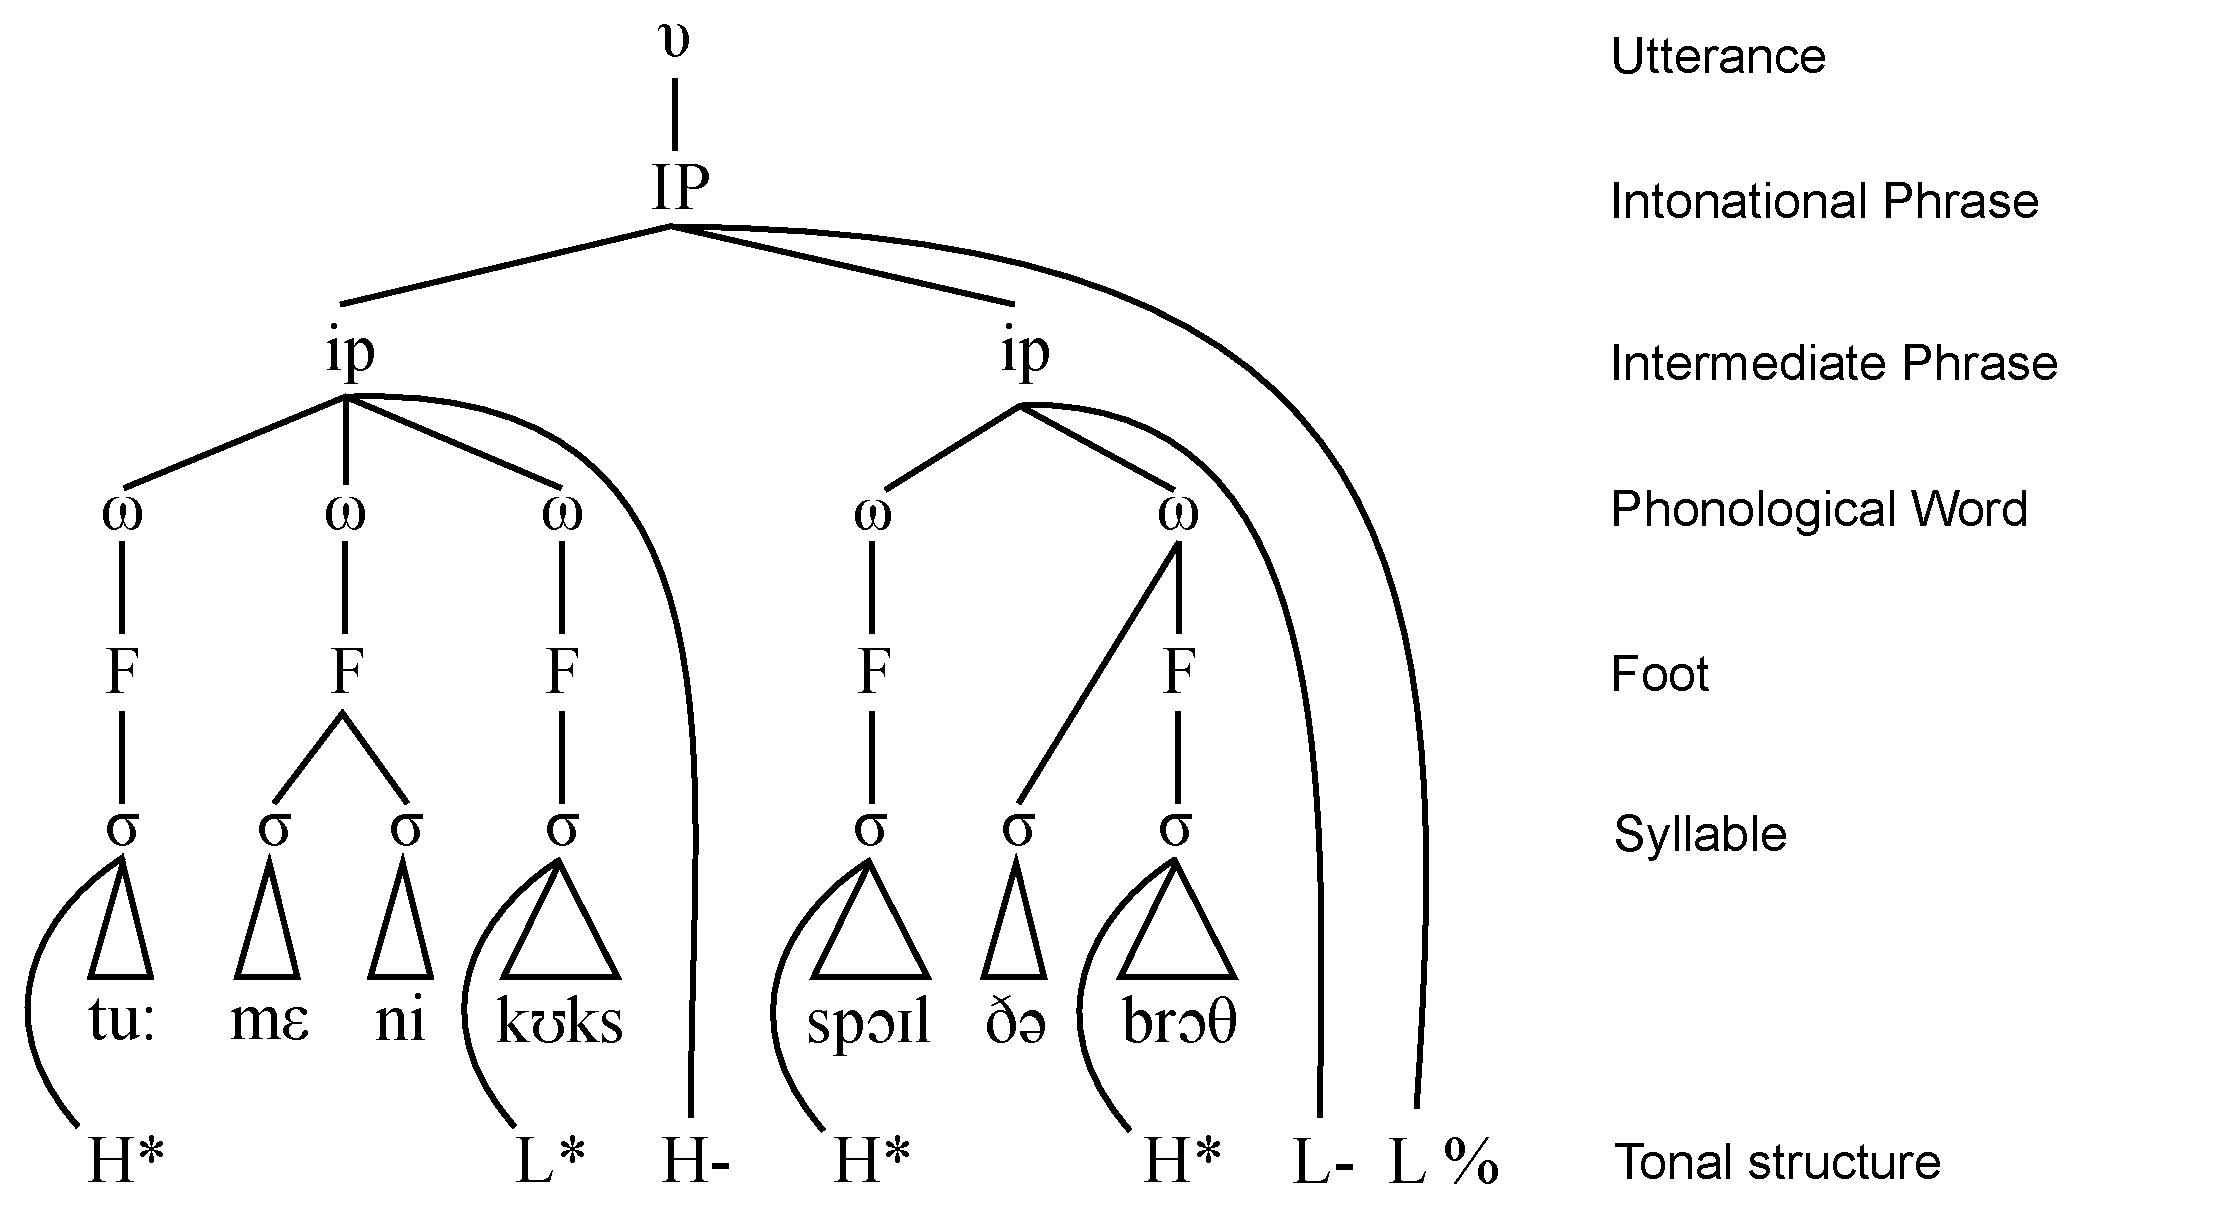
\includegraphics[width=\textwidth]{figures/ch4/prosodic_hierarchy.pdf}
\caption{Prosodic hierarchy for the sentence ``too many cooks spoil the broth" inspired by \citet{Grice2006} and \citet{Gussenhoven2004}.}
\label{fig:prosodic_hierarchy}
\end{figure}

An intonation contour in the AM framework is modelled as a string of high and low tones, H and L, that is associated with the constituents in the prosodic hierarchy. However, not every word or syllable in a phrase receives a tone. The string of tones is associated with the ``text", i.e. the syllables of a sentence, at certain points. Between the syllables where tones occur, the intonation contour is interpolated \citep{Ladd2008}. 

Tones can occur as \emph{pitch accents} or as \emph{boundary tones}. In many intonational languages -- like English, German and Dutch -- pitch accents are associated with primary stressed syllables in the prosodic hierarchy. The term pitch accent is used here in the sense of \emph{intonational pitch accent} as opposed to \emph{lexical pitch accent} \citep{Ladd2008}. Intermediate phrases can contain more than one pitch accent. Of all pitch accents, the last (fully fledged) pitch accent is called the \emph{nuclear pitch accent} \citep{Gussenhoven2004}. The placement of the nuclear pitch accent can be seen as a form of head-marking \citep{BeckmanEdwards1994, ShattuckHufnagelTurk1996} in which the most prominent syllable of the intermediate phrase is the head of this prosodic constituent and receives the nuclear pitch accent \citep{Grice2006}. A pitch accent is marked by the symbol * and can consist of one or two tones, e.g. H* or L+H*. In the latter case, i.e. in bitonal pitch accents, only one of the two tones receives the * and is called the \emph{starred tone}. The other tone occurs either before the starred tone, as in the case of a \emph{leading tone} (L+H*), or after the starred tone, as in the case of a \emph{trailing tone} (L*+H). 

Boundary tones occur on two levels. Both intermediate and intonation phrases have boundary tones. One convention (see for example GToBI: \citealp{GriceBaumann2002} and \citealp{GriceBaumannBenzmüller2005}) is to mark the boundary tone of an intermediate phrase with the symbol -, e.g. L-, and the boundary tone of an intonation phrase with the symbol \%, e.g. L\%. Since intermediate phrases are contained in intonation phrases, the end of an intonation phrase co-occurs with the end of the last intermediate phrase of the intonation phrase. The notation of the two boundary tones is T$_1$-T$_2$\%, where T stands for tone. If T$_1$ and T$_2$ are identical, only one of them is written, i.e. L-L\% is written as L-\%. 

The motivation of modelling an intonation contour as a string of tones rather than a holistic melodic unit comes from the observation that the intonation contour is not simply stretched or compressed when the number of syllables present in the sentence increases or decreases. Instead, the shape of the intonation contour is affected by the alignment of the tones relative to the syllables they are associated with \citep{Ladd2008, Arvaniti2011}. The example in Figure \ref{fig:me_ballgown} illustrates this point: It shows a schematised version of a contour prominently discussed in the literature by \citet{HirschbergWard1985}, \citet{HirschbergWard1992}, \citet{Arvaniti2011}, \citet{Ladd2008} and many others. The contour is used to express incredulity towards a suggestion made by the interlocutor. On the left, the realisation on the mono-syllabic phrase ``Me?!” is shown. The intonation contour rises, falls and rises again. This contour could be described as a holistic rise-fall-rise pattern \citep{Ladd2008}. On the right, the figure shows two options of adjusting the contour to be realised on a longer phrase. In the upper plot, the holistic rise-fall-rise shape of the contour is simply stretched to span the longer phrase. However, this is not the way the contour is realised on longer phrases \citep{Arvaniti2011}. The actual realisation of the contour is represented by the schematisation in the lower plot and demonstrates that the contour is best described as a composition of separate tonal events. The phrase starts low, the rise-fall movement is timed roughly with the syllable ``ball” and not stretched over several syllables. The final rise of the contour is realised at the very end of the utterance, most probably on the last syllable of ``designer”. There is a low stretch of F0 in between these two events. An analysis within the AM framework decomposes this contour into a pitch accent and a rising boundary tone at the end of the phrase. The pitch accent is associated with the most prominent syllable in the phrase, ``ball”, and gets aligned with it in time. The boundary tone is associated with the phrase and marks the edge of this phrase. As a consequence, its rising tonal movement is realised towards the end of the phrase. In between these two tonal events, the low stretch of F0 represents an interpolation that can be extremely short as in the case of ``Me?!" or longer depending on the number of syllables between the accent and the edge \citep{Ladd2008} . 

\begin{figure}[h]
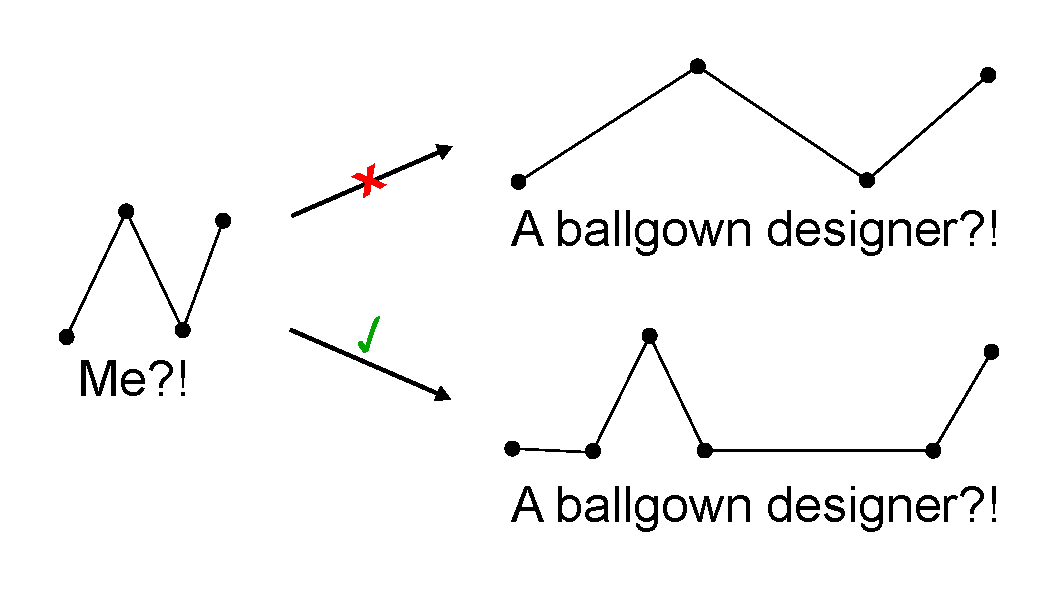
\includegraphics[width=8cm]{figures/ch4/me_ballgown.pdf}
\caption[Schematic illustration of an intonation contour expressing incredulity.]{Schematic illustration of an intonation contour expressing incredulity \citep{HirschbergWard1992}. The right side shows two hypothetical options how the short version can be enlarged for longer sentences.}
\label{fig:me_ballgown}
\end{figure}

\largerpage\largerpage
A possible analysis in the AM tradition \citep[as in ToBI:][]{BeckmanHirschbergShattuckHufnagel2005} would describe the contour as L*+H L-H\%\footnote{The fact that the phrase starts low is accounted for with a default boundary tone that is described as mid or low in the speaker's range and, being the default, is omitted from the transcription.} with the L of the boundary tone spreading ``leftwards" to the end of the pitch accent to create a low stretch on the non-prominent syllables after the pitch accent. Depending on the inventory of pitch accents and boundary tones (e.g. presence of leading and/or trailing tones), models in the AM framework can differ in their description of the same contour. The common assumption, however, is that the contour can be decomposed into tonal events and that such a description is better able to capture generalisations on intonational structure and meaning than a holistic approach.  

\section{A first look at prosodic focus marking}
\label{sec:focus1}

In West-Germanic languages, like German, Dutch and English, the placement of a pitch accent is used as a means to package the information conveyed by a sentence. In these languages, prosody plays a role in signalling which parts of the utterance are in \emph{focus}, and which are in the \emph{background} \citep{Lambrecht1994}. This structure, the \emph{focus structure} of the sentence, manifests the speaker's beliefs about how the information of the sentence fits the knowledge of the listener \citep{Vallduvi1992}. The focus constituent includes the information that the speaker believes to be significant, the background constituent contains information that is less relevant \citep{Gussenhoven2004}. Often, the focus constituent contains new information while the background contains given information, but this is not always the case. In the above-mentioned languages, the focussed part usually receives the nuclear pitch accent. The background constituent usually does not receive the nuclear pitch accent and is often completely unaccented, in particular when the background part follows the focus part (\largerpage{}also known as \emph{post-focal deaccentuation}).

Consider the example in \ref{ex:broad_focus}. The answer contains only new information \citep{Ladd1980, Gussenhoven2004}, nothing is given by the question, everything is in focus. This condition is often called \emph{broad focus} \citep{Ladd1980}. In this case, the nuclear pitch accent is usually placed on the last noun, ``Jana”. Even though ``Jana" receives the nuclear pitch accent, this does not mean that it is the only word in focus. The mechanism that assigns the nuclear pitch accent within the focussed constituent is called \emph{focus projection} \citep{Büring2003, Ladd2008}. The word that receives the nuclear pitch accent functions as the \emph{focus exponent} for the larger focus domain \citep{Ladd2008}. 

\begin{equation}
\begin{tabular}{ll}
Q: & 	Was gibt’s Neues?\\
&	What’s up?\\
A: &	[Melanie will Jana treffen.]$_F$\\
&	[Melanie wants to meet Jana.]$_F$
\end{tabular}
\label{ex:broad_focus}
\end{equation}

In example \ref{ex:narrow_focus}, the question triggers a different focus structure in the answer. The new information is contained in the word ``Jana” only. The focus structure of this example is called \emph{narrow focus} \citep{Ladd1980, Gussenhoven2004}. As in the example before, the pitch accent is placed on the word ``Jana".

\begin{equation}
\begin{tabular}{ll}
Q: & 	Wen will Melanie treffen?\\
&	Who does Melanie want to meet?\\
A: &	Melanie will [Jana]$_F$ treffen.\\
&	Melanie wants to meet [Jana.]$_F$
\end{tabular}
\label{ex:narrow_focus}
\end{equation}

A special case of narrow focus is illustrated in example \ref{ex:contrastive_focus}. Again, all information except for ``Jana” is given by the question. In addition, ``Jana” serves as a direct alternative to the referent ``Peter” given in the question. The nuclear pitch accent is again placed on the word ``Jana”. This focus structure is often labelled \emph{contrastive focus} or \emph{corrective focus} \citep{Gussenhoven2004}.

\begin{equation}
\begin{tabular}{ll}
Q: & 	Will Melanie Peter treffen?\\
&	Does Melanie want to meet Peter?\\
A: &	Melanie will [Jana]$_F$ treffen.\\
&	Melanie wants to meet [Jana.]$_F$
\end{tabular}
\label{ex:contrastive_focus}
\end{equation}

So far, the pitch accent location did not change in the examples as a function\largerpage{} of the focus structure of the sentence. Either the last noun was the only focussed element (narrow and contrastive focus) or it served as the focus exponent for a larger focus domain (broad focus). Example \ref{ex:background} demonstrates what happens if the focus is earlier in the sentence. The example in fact shows a case of contrastive focus. This time, however, the focussed element is ``Melanie”. As a consequence, the nuclear pitch accent is placed on ``Melanie” and the part of the utterance after this word, ``will Jana treffen”, is in the background. This part is deaccented and characterised by a low stretch of F0, lower amplitudes and shorter durations.

\begin{equation}
\begin{tabular}{ll}
Q: & 	Will Paul Jana treffen?\\
&	Does Paul want to meet Jana?\\
A: &	[Melanie]$_F$ will Jana treffen.\\
&	[Melanie]$_F$ wants to meet Jana.
\end{tabular}
\label{ex:background}
\end{equation}

Moving the nuclear pitch accent to a different word as a means of packaging the information is a very well described phenomenon in intonation languages like English, German and Dutch. Other intonation languages like Spanish and Italian do not use the manipulation of the nuclear pitch accent location to mark focus structure or do so only to a limited extent \citep{Ladd2008}. Languages that use nuclear pitch accent location to mark focus have been called \emph{plastic} languages, those that do not have been called \emph{non-plastic} languages \citep{Vallduvi1991}.

Although manipulating the location of the nuclear pitch accent is a very well documented and salient feature of focus marking, this is not to say that focus structures with the nuclear pitch accent in the same place are identical with regard to their prosodic realisation. Later in this chapter, evidence for fine-grained strategies of prosodic focus marking will be discussed. The second part of this book presents a large data pool supporting and extending this evidence. It will become clear that both categorical and continuous modulations are used in the differentiation of focus structures. Therefore, before turning to this central issue, it is useful to take a closer look at what is known about categorical and continuous characteristics of prosody. 

\section{The nature of prosody: categorical and continuous}
\label{sec:prosody_catcont}

The outlined view of intonation in the AM framework is characterised by the assumption of discrete events in tonal structure. The last two sections sketched the motivation for this perspective. First, as illustrated by the example of the ``incredulity contour" (see Figure \ref{fig:me_ballgown}), it is plausible to analyse intonation contours as composites. Some units that form these composites are associated with strong syllables while others are associated with phrase constituents. Hence, the wide-spread approach of AM intonation analysis posits that categoriality is a major feature of the structure of intonation contours: Tones can belong to the categories pitch accent or boundary tone. 

Second, the examples of focus realisation in German (\ref{ex:broad_focus}, \ref{ex:narrow_focus}, \ref{ex:contrastive_focus}, and \ref{ex:background}) have added another important aspect of categorical patterning in the analysis of intonation. It is a discrete choice which syllable a pitch accent (in this case the nuclear pitch accent) is associated with. The pitch accent is either associated with syllable A or B (or C or...). Moreover, different types of pitch accents exist in the AM analysis. This means that while there is a possible syntagmatic contrast between a syllable that receives a pitch accent and one that does not, there are also possible paradigmatic contrasts between pitch accent types. A pitch accent can be of type A or B (or C or...), or in AM terms: H* or L* or H+L* (or L+H* or...). Models within the tradition of AM draw pitch accents from a closed inventory and consider these pitch accent types as phonologically distinct. Analogously, boundary tones are also given as a closed set of distinctive types.

The identification of categoriality in the structure of intonation forms the basis of the ``intonational phonology" \citep{Ladd2008} put forward by scholars in the AM framework. However, it is not restricted to this framework and has antecedents in other models. For instance, intonation analysis in the tradition of the \emph{British School} \citep{OConnorArnold1973} identifies categorical distinctions on multiple levels. Pitch accented syllables are distinguished from other categories of prominence (secondary stress, tertiary stress, unstressed). Moreover, intonation contours are decomposed into parts like head, nucleus and tail. With regard to the \emph{nuclear tone}, consisting of the nucleus and the tail, the British School has attempted to identify distinct tunes that evoke differences in meaning, like ``high fall" or ``low rise" \citep{Cruttenden1997}. In the \emph{IPO} model of intonation \citep{tHartCollierCohen1990} -- named after the Institute of Perception Research, in Dutch: Instituut voor Perceptie Onderzoek -- similar to the analysis of the AM framework, a distinction is made between pitch movements associated with boundaries and pitch movements associated with prominences. Tonal patterns are described in terms of a composition of ``categorically distinct entities" \citep[14]{Ladd2008}, e.g. ``Type A Fall" or ``Type 1 Rise". 

To conclude, the assumption of the categorical, phonological status of intonation contours or building blocks of contours plays a significant role in various aspects of the description of intonation. Experimental approaches have been developed to assess the notion of categoriality in intonation empirically. For example, \citet{PierrehumbertSteele1989} manipulated the timing of the accentual peak of a rise-fall-rise contour on the sentence ``Only a millionaire" from relatively early to relatively late with 13 intermediate steps.\footnote{The ``relatively early peak" L+H* in this experiment should not be confused with the general notion of an early peak accent that is usually transcribed as H+L* or H+!H*.} The resulting 15 stimuli represented a continuum between two contours that can be described as L*+H L-H\% and L+H* L-H\% with the pitch accent associated with the syllable ``mil". Apart from the alignment of the accentual peak with the accented syllable, the contour was unaltered. The subjects participating in the study were asked to listen to a stimulus and imitate it. The authors' prediction was the following: If the nature of the difference between the two pitch accent types is categorical, the subjects should not be able to reproduce the continuum exactly. The data should instead cluster around two alignment patterns, one representing L*+H and the other one representing L+H*. If, on the contrary, alignment is used as continuous dimension in the intonation of American English, the subjects should be able to reproduce the continuum faithfully.

The result showed that almost all participants produced patterns that more or less clustered around two points on the continuum of peak alignment, yielding bimodal distributions for almost all speakers. Interestingly, although the results of the study suggest that peak alignment is used in a categorical fashion rather than continuously, two interesting observations can be made. First, the relative sizes of the two modes of the bimodal distributions differ across speakers, indicating that the continuum of stimuli is divided differently by individual speakers. Most speakers categorise a larger portion of the continuum as L+H* but there is also one speaker that divides the continuum into two approximately equal parts. Second, the modes of the alignment distributions of individual speakers are located differently in time. Both observations show that categories like L*+H and L+H* are not invariantly linked to patterns of phonetic implementation. 

Results pointing towards a categorical use of tonal alignment were also obtained by \citet{DImperioHouse1997}, investigating the intonation of narrow focus statements and yes/no questions in Neapolitan Italian. In this variety of Italian, both narrow focus statements and yes/no questions are characterised by a rising nuclear pitch accent followed by low boundary tone. The pitch accent of the narrow focus statement is analysed as H* while the pitch accent of the yes/no question is analysed as L+H*. According to \citet{DImperioHouse1997}, this difference is at least partially expressed with respect to timing of tonal events: The accentual peak of the H* is reported to be reached earlier than the peak of L+H*. The stimuli of this study comprise a five step continuum from relatively early (H*) to relatively late peak (L+H*). One set of stimuli was synthetically produced on the basis of the natural production of a statement and another set was produced on the basis of a question.

In contrast to \citet{PierrehumbertSteele1989}, a different experimental design was employed by \citet{DImperioHouse1997} to elicit the subject's responses. Participants were asked to listen to the continuum and categorise the stimuli they just heard as a question or a statement. The results showed that subjects categorise the earlier peak (H*) as a narrow focus statement and the later peak (L+H*) as a yes/no question as expected. Around the mid-point of the continuum, the proportions of ratings for both categories are around 50\% and the variability in the responses is high -- a response pattern expected for categorical oppositions. It should be noted, however, that these effects are clearest for stimuli that were resynthesised from a natural production of a statement. Additional evidence for the role of temporal alignment in the categorisation of pitch accent types comes from \citet{DilleyHeffner2013} for American English as well as \citet{Kohler1987} for German.

\citet{GussenhovenRietveld2000} provided support for categoriality of pitch accents in Dutch. The authors investigated the difference between a ``high rise" and ``low rise" question contour. In the former contour, the nuclear accented syllable is mid-pitched. In the latter contour, the nuclear accented syllable is low. Both contours are characterised by a rise from the accented syllable to the end of the phrase. In terms of an AM analysis, the contours could be described as H* H-H\% and L* H-H\% \citep{Gussenhoven2004}. The experimental paradigm of \citet{GussenhovenRietveld2000} is based on the observation that speakers expand the pitch range when speaking in an emphatic or surprised fashion. Accordingly, subjects were presented with artificial contours in which the height of both the accentual target (L* or H*) and the boundary tone target (H-H\%) were manipulated. 

The results are in line with the prediction that what is analysed as a phonological low tone (L) behaves differently from what is analysed as a phonological high tone (H) when the pitch range is expanded. A L* accent is perceived as ``more surprised" when realised lower whereas a H* accent is perceived as ``more surprised" when realised higher. These results suggest that it is plausible to describe the accent as belonging to two different categories. At the same time, they reveal that intonational meaning, in this case ``surprise", is carried by continuous variation as well. In addition, the results of \citet{GussenhovenRietveld2000} show that the implementation of categories is subject to contextual variation and not invariant.

The experiment of \citet{GussenhovenRietveld2000} was based on the assumption that pitch range constitutes a parameter continuously varied by speakers. \citet{LaddMorton1997} questioned the purely continuous nature of pitch range as a parameter of intonation. The authors sought empirical evidence for the existence of \emph{normal} and \emph{emphatic} peak pitch accents as two distinct categories in British English. This distinction is assumed to be (at least partially) expressed by pitch range with the emphatic accent having a larger pitch range than the normal accent. Since in this study phrases with only one accent are used, it remains open whether pitch range is interpreted ``globally" on the level of the phrase or ``locally" on the level of the accent. Regardless of which interpretation is to be favoured, one can speak of a difference in \emph{pitch excursion}, manifested phonetically in the relation between the F0 target of the peak on the accented syllable and the F0 target of the low boundary following.

The findings of \citet{LaddMorton1997} on the categorical use of pitch excursion remain inconclusive and thereby provide an interesting example of the study of categoriality and continuity in intonation. The methodology of the study included both rating on a scale as well as forced choice tasks. In a first perception experiment -- which was designed to be a norming study to test the usefulness of the speaker's voice and the manipulation strategies -- the authors randomly played stimuli from a continuum of pitch excursions to 35 subjects. This continuum consisted of resynthesised contours based on natural utterances produced in either a ``normal" or an ``emphatic" fashion. The pitch excursion on the continuum was increased in steps of 6 Hz. Two instructions to elicit the participants' answers were used. In the first instruction, the participants were asked to rate the degree of emphasis on a ten-point scale. In the second instruction, two different interpretations were presented, ``a neutral statement" and ``a contradiction or correction". The participants were asked to rate on a ten-point scale how likely the interpretations were. The results show that stimuli manipulated from an emphatic natural basis were interpreted as more emphatic, a finding that indicates that emphasis is expressed by more than just pitch excursion. Apart from this effect, both sets of stimuli evoked similar responses: The larger the pitch excursion, the more ratings towards an ``emphatic" interpretation. This trend showed no clear discontinuities that would be expected for a categorical difference.

In a second experiment, \citet{LaddMorton1997} used a subset of the stimuli from the first experiment and employed a classic categorical perception paradigm consisting of two forced choice tasks, an \emph{identification task} and a \emph{discrimination task}. In the identification task, subjects listened to a stimulus from the continuum and judged whether the sentence described an ``everyday occurrence" or an ``unusual experience". In the discrimination task, subjects listened to pairs of stimuli in quick succession and were asked to choose whether they were the same or different. The stimuli of a pair were either neighbours on the manipulated continuum and thus differed by 6 Hz or were identical. 

The responses of the identification task provided the classic S-shaped curve expected for the presence of two categories. The curve showed that in the region between 138 and 156 Hz, the responses abruptly become more variable and tend towards 50\%, i.e. subjects were less certain about the interpretation of the stimuli. This result alone does, however, not suffice to attest the existence of two distinct categories of normal and emphatic. It has to be kept in mind that the subjects had only two options to choose from. To provide clearer evidence for categoriality, the discriminability of stimuli must increase in the region of the putative category boundary. Remember that the pairs of different stimuli played in the discrimination task consisted of neighbours on the continuum differing by 6 Hz. Subjects should perform better at discriminating stimuli belonging to different categories compared to stimuli belonging to the same category. In fact, in the study of \citet{LaddMorton1997}, subjects were better at discriminating stimuli pairs at the putative category boundary. However, the discrimination rate was rather low even in this region. In addition, the discrimination rates at the ends of the acoustic continuum, i.e. within the assumed categories, were also larger than zero.

While the findings of \citet{LaddMorton1997} do not support categorical perception of normal and emphatic pitch accents in a strict sense, they suggest that the continuum was not completely linearly perceived. These observations reflect the fact that pitch excursion may be used in a categorical and continuous way at the same time. For example, transcription systems in the AM tradition acknowledge that H* and L+H* accents are, among other parameters, distinguished in terms of in the magnitude of the rise towards the starred tone H* \citep{GriceBaumann2002}. The rise is described as steeper and higher for L+H* compared to H*. Thus, in this case, local pitch excursion is one phonetic parameter to differentiate phonological categories. At the same time, this parameter is used in a continuous fashion. The continuous use can be the result of global or local pitch range expansions to signal emotional affection or surprisal (as in the case of Gussenhoven and Rietveld's experiment) or to make a distinction between different accent types clearer. The latter case might be classified as a kind of intonational hyperarticulation in the sense of Lindblom's (\citeyear{Lindblom1990}) Hyper- and Hypo-Articulation theory (H\&H theory).

Striking similarities are found for the phonetic parameter of temporal alignment of an accentual peak. At the beginning of this section, evidence has been presented for the existence of a categorical implementation of this parameter. However, it is also known that later alignment of an accentual peak may be used in addition to increased pitch excursion -- or even as a substitute for increased pitch excursion -- to increase prominence in intonation languages like German and English \citep{Gussenhoven2004, LaddMorton1997}. A possible explanation might be that higher pitch excursions take longer to be executed. Therefore, higher peaks have a potential physiological correlate of delay, a mechanism that speakers may have ``tacit knowledge" of \citep[90]{Gussenhoven2004}. Regardless of the validity of this explanation, the observation is interesting for two reasons. First, it shows that alignment is used in a continuous manner as well. Second, while the symbiosis of pitch excursion and alignment is conceptualised as a phonetic effect, it is also manifested in the description of intonational categories: In addition to a difference in the magnitude of the rise towards the high accentual target (as already mentioned above), the distinction of H* and L+H* in German ToBI is based on a difference in alignment. A later peak alignment is attributed to the L+H* accent in comparison to the H* accent in this model.

Essentially, these observations suggest a deep intertwining of the use of prosodic parameters to establish phonological categories on the one hand and their direct, continuous (or: phonetic) use on the other. The next section will present evidence on the realisation of focus types that provides support for the idea of an interrelation of phonetic and phonological aspects of intonation developed in the present section.

\section{A closer look at prosodic focus marking}
\label{sec:focus2}

Earlier in this chapter, the use of nuclear pitch accent placement in West-German\-ic languages to mark focus structure was introduced. It was noted that the placement of the nuclear accent might not change as a function of focus structure in some cases. In the examples, the nuclear accent remained on the word ``Jana", the last noun, regardless of whether the focus structure was broad focus, narrow focus or contrastive focus. The literature nevertheless discusses prosodic ways of  differentiation between these focus types.

For American English, \citet[296]{PierrehumbertHirschberg1990} state that the L+H* pitch accent ``evokes a salient scale". It is described to mark contrastive focus as opposed to the H* accent that -- combined with a low boundary tone -- contributes to a ``neutral declarative intonation" \citep[290]{PierrehumbertHirschberg1990}. \citet{WatsonTanenhausGunlogson2008} add supporting evidence for the interpretation of L+H* as marking contrastive focus in an eye-tracking study. They note, however, that the uses of L+H* and H* seem to overlap.

For German, \citet{Baumannetal2007} found that the proportion of downstepped H* accents, i.e. !H*, is highest in broad focus. The number of upstepped H* accents, \^{}H*, is highest in contrastive focus. Plain H* accents are predominantly found in narrow focus. While the distributions are overlapping, in line with the perceptual findings of \citet{WatsonTanenhausGunlogson2008}, these results by \citet{Baumannetal2007} indicate that different pitch accent types are used to signal different focus types. Crucially, the predominantly used accent types are characterised by increasing acoustic salience from broad focus to narrow focus, and from narrow focus to contrastive focus \citep[see][]{BaumannRöhr2015}. The results are supported by data presented in \citet{BaumannGriceSteindamm2006} that show fewer downstepped accents in narrow compared to broad focus, and fewer downstepped accents in contrastive compared to narrow focus. 

Contrary to these findings, \citet[63]{Fery1993} reported no difference between broad and narrow focus. The divergence of the results might be attributed to the fact that the speech material of this study is different from the sentences used in above-mentioned studies by \citet{Baumannetal2007} and \citet{BaumannGriceSteindamm2006} (and the examples given earlier in the present chapter). Another explanation might be sought in the fact already mentioned several times in this discussion: The distributions of pitch accent types used for different functions are overlapping. Hence, there does not seem to be a one-to-one mapping of pitch accent type to focus type.

\citet{Griceetal2017} investigated the categorical and continuous aspects of intonational patterns used to mark focus structures by 5 German speakers (data also reported on in \citealp{MückeGrice2014}). The speech material used was very similar to the examples \ref{ex:broad_focus}, \ref{ex:narrow_focus}, and \ref{ex:contrastive_focus}. Their analysis comprised both symbolic annotations as well as measurements of continuous, phonetic parameters. Figures \ref{fig:grice_etal_2017_PA_types} and \ref{fig:grice_etal_2017_PA_types_speakers} give a first insight into their data by showing the GToBI nuclear pitch accent distributions based on consensus annotations by two annotators. Figure \ref{fig:grice_etal_2017_PA_types} gives the distributions for all speakers together and confirms the finding outlined above, namely that there is not a one-to-one mapping of pitch accent type to focus type but that there are tendencies: Most falling accents, H+!H*, can be found in broad focus, most accents with a steep rise, L+H*, can be found in contrastive focus. Narrow focus seems to be positioned in between with a rather high number of H* accents but also a considerable number of L+H* and even H+!H* accents. Figure \ref{fig:grice_etal_2017_PA_types_speakers} presents the distributions for each speaker separately. While for some speakers (F1 and F2) the overall tendency of Figure \ref{fig:grice_etal_2017_PA_types} can be observed at least for the differentiation of broad focus and contrastive focus, for other speakers (F3 and M2), a different picture is obtained. These speakers use one pitch accent category predominantly for all three focus types. In the case of speaker F3, it is H*; in the case of speaker M2, it is L+H*. Speaker M1 seems to use a mixed strategy between the two groups. This speaker differentiates broad and\largerpage{} narrow focus by using different pitch accent types, but shows almost exclusively L+H* accents in both narrow and contrastive focus.

\begin{figure}[p]
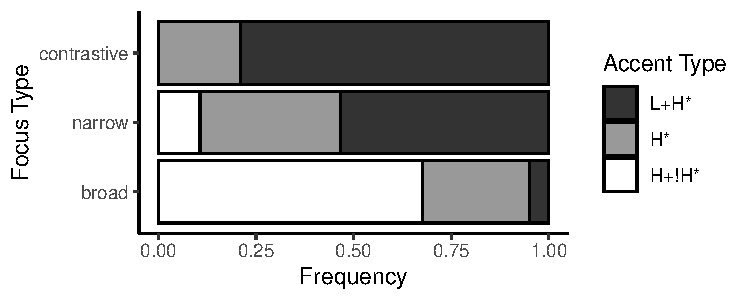
\includegraphics[width=10cm]{figures/ch4/Grice_etal_PA_Types.pdf}
\caption{Nuclear pitch accent type distributions in the data set of \citet{Griceetal2017}.}
\label{fig:grice_etal_2017_PA_types}
\end{figure}

\begin{figure}[p]
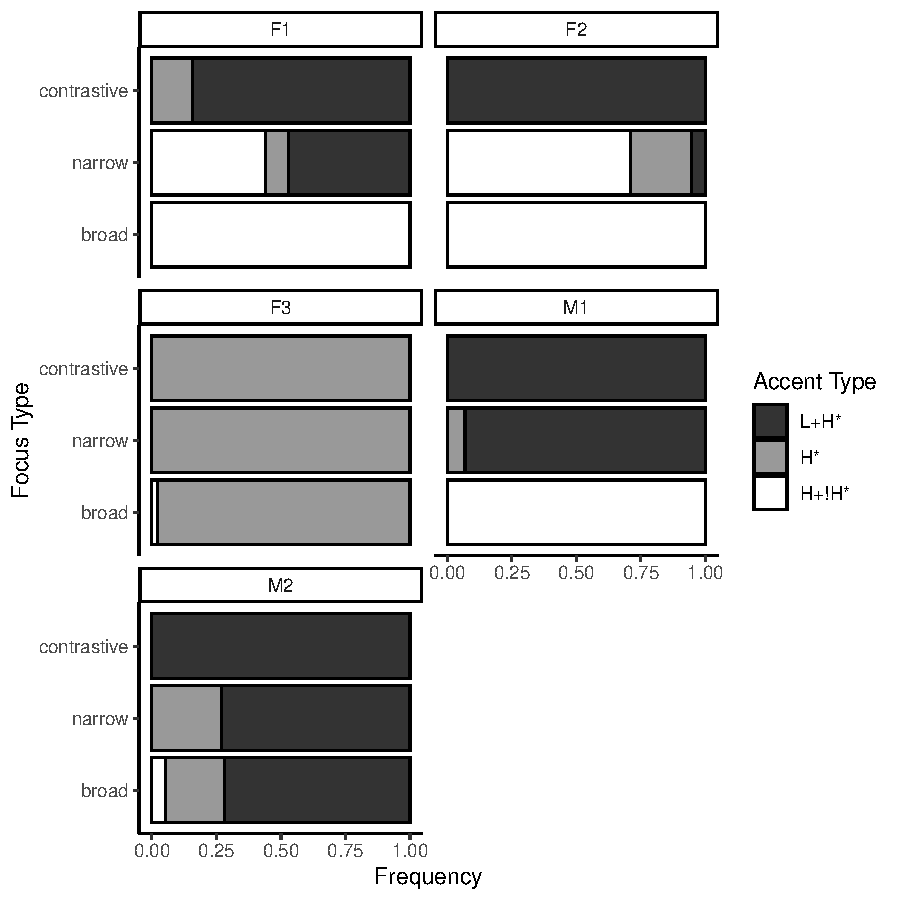
\includegraphics[width=.9\textwidth]{figures/ch4/Grice_etal_PA_Types_Speakers.pdf}
\caption{Nuclear pitch accent type distributions in the data set of \citet{Griceetal2017} for each speaker separately.}
\label{fig:grice_etal_2017_PA_types_speakers}
\end{figure}

The data of \citet{Griceetal2017} was used in a perception test by \citet{CangemiKrügerGrice2015} and \citet{Krüger2009}. Their results showed that all five speakers were ``able to convey their pragmatic intentions to listeners in a comparable way" \citep[91]{Griceetal2017}. This conclusion is rather surprising with regard to the different pitch accent distributions and considering that some speakers do not differentiate the focus types clearly in terms of their pitch accent choice. Motivated by the discrepancy of pitch accent choice and scores in perception testing, the analysis by \citet{Griceetal2017} went beyond the description of intonational patterns using pitch accent types and investigated various continuous parameters. Interestingly, their results reveal that the speakers' strategies are not as disparate as the pitch accent distributions suggest. Figure \ref{fig:grice_etal_2017_alignment} shows the mean alignment values of the peak of the nuclear pitch accent in relation to the onset of the accented syllable.\footnote{The original paper uses the alignment relative to the accented vowel onset which yields comparable results. The current figure is based on the openly available data set which contains both alignment relative to the onset of the accented syllable (that has a CV structure) as well as alignment relative to the onset of the accented vowel.} Note that the peak does not have to belong to the starred tone (as in the case of H* and L+H*). In H+!H* accents, the peak is part of the leading tone (H+). The alignment data reveal the same pattern for all five speakers: Broad focus has the earliest peak alignment, contrastive focus has the latest peak alignment, narrow focus is in between the two extremes: broad < narrow < contrastive. For the speakers that showed pitch accent type differentiation (F1 and F2, partly M1), the alignment modification ``crosses" category boundaries of pitch accent types. H+!H* accents in broad focus, for example, contribute negative alignment values as opposed to clearly positive values for L+H* accents in contrastive focus. For the other speakers (F3 and M2, partly M1), the alignment is modified within the boundaries of a single category. In other words, the parameter alignment is used in both continuous, ``phonetic" and categorical, ``phonological" ways but the general trend of modification, or the direction of modification, is invariant across speakers.

\begin{figure}
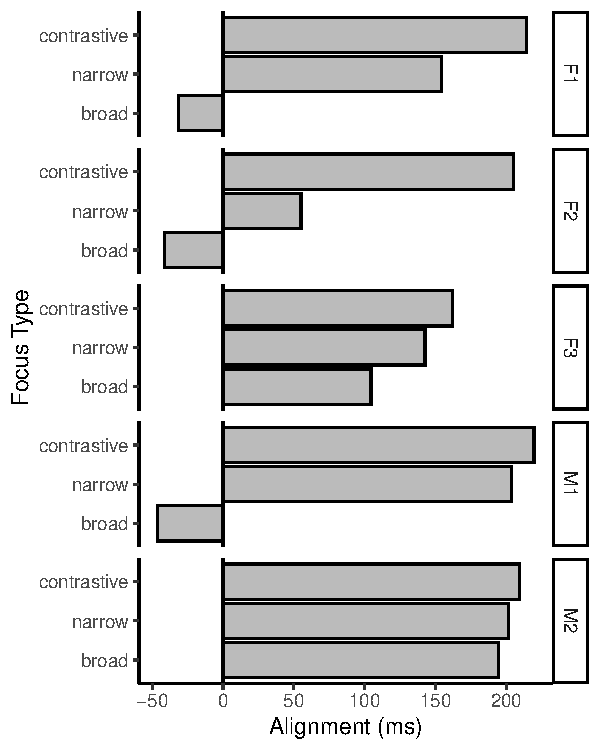
\includegraphics[width=9cm]{figures/ch4/Grice_etal_Alignment.pdf}
\caption{Mean alignment of the peak relative to the onset of the accented syllable in the data set of \citet{Griceetal2017} for each speaker separately.}
\label{fig:grice_etal_2017_alignment}
\end{figure}

In addition to the alignment of the peak, \citet{Griceetal2017} measured the \emph{tonal onglide} \citep{RitterGrice2015}, a parameter that plays an important role throughout the following parts of this work. The tonal onglide is a means to assess the F0 movement towards the main tonal target of the accent -- in AM terms, the starred tone. In the version that \citet{Griceetal2017} employed, the tonal onglide is quantified as the difference in semitones between the starred tone target and a fixed point 30 ms before the onset of the accented syllable. If the accent is falling, the resulting tonal onglide is negative, if the accent is rising, the tonal onglide is positive. This means that the tonal onglide gives an indication of the movement of the accent (falling vs. rising) but also of the magnitude of this movement. It is comparable to the measure of alignment by answering the question whether the accent is an early peak accent like H+!H* or a mid to late peak accent like H* or L+H*. But it also assesses pitch excursion continuously, for example by quantifying the magnitude of the rise in accents like L+H*.

In Figure \ref{fig:grice_etal_2017_onglide}, the results of the tonal onglide measure from \citet{Griceetal2017} are shown. The picture obtained here is comparable to the results for the peak alignment -- it is even clearer in some cases. All speakers manipulate the tonal onglide in the same direction. Broad focus has the smallest tonal onglide values, contrastive focus has the largest, narrow falls in between: broad < narrow < contrastive. As in the case of alignment, some speakers cross clear category boundaries. For example, the negative tonal onglide values of F1, F2 and M1 in broad focus are an indication of accents of the falling type H+!H* whereas the positive onglide values in contrastive focus result from the frequent use of the rising accent type L+H*. Crucially however, a speaker like F3 that exhibits only H* accents in the categorical analysis of Figure \ref{fig:grice_etal_2017_PA_types_speakers} differentiates the focus types in terms of onglide values. The same is true for speaker M2 and the difference between narrow and contrastive focus in speaker M1.

\begin{figure}[t]
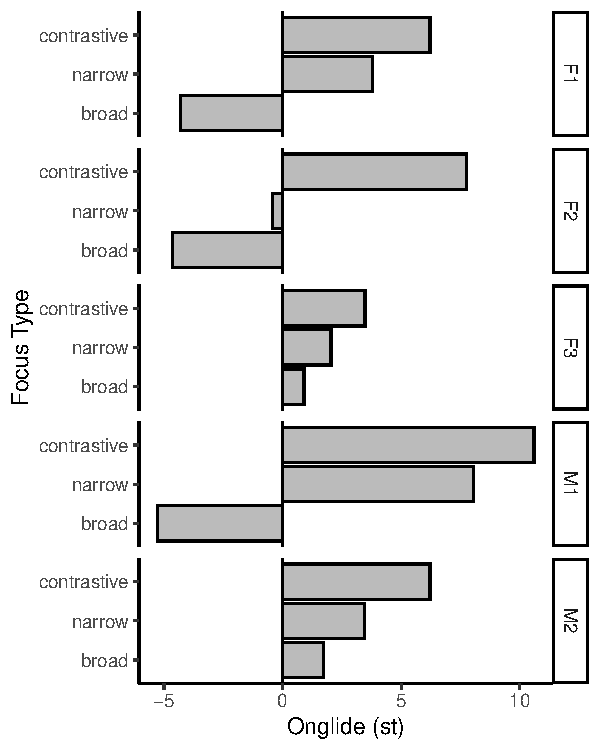
\includegraphics[width=9cm]{figures/ch4/Grice_etal_Onglide.pdf}
\caption{Mean tonal onglide values in the data set of \citet{Griceetal2017} for each speaker separately.}
\label{fig:grice_etal_2017_onglide}
\end{figure}


Both alignment and tonal onglide give a deeper insight into strategies of focus marking. What appears to be disparate strategies in a symbolic account is shown to be very similar when looking at the continuous parameters in addition to the symbolic transcription. Moreover, the results suggest that there might be no clear boundary between a categorical and a continuous use of intonation to mark focus types. Rather, speakers seem to integrate the two uses with a clear mutual trend. As the perception results of \citet{CangemiKrügerGrice2015} and \citet{Krüger2009} show, listeners are able to use the information encoded in the speech signal, regardless of whether the differences are in terms of what is described as pitch accent categories or more subtle and subsymbolic variation. This finding resonates well with the remark of \citet[88]{Ladd2014} discussed in Chapter \ref{chapter_pandp} that categorical and continuous variation commonly go hand in hand and very often ``are likely to interact and reinforce one another".

\section{Prosodic strengthening}
\label{sec:prosodic_strengthening}

So far, this chapter has concentrated on tonal aspects of prosody. A large body of research shows, however, that many other aspects play an important role as well. One important aspect is that the articulation of consonants and vowels -- also often called \emph{supra-laryngeal} articulation as opposed to \emph{laryngeal} articulation that produces tone -- is affected by prosodic structure \citep{Mücke2018}. More specifically, it has been shown that some positions in the prosodic hierarchy are characterised by ``stronger" articulation to increase syntagmatic and paradigmatic contrasts. Often, articulatory gestures are expanded in the spatio-temporal domains \citep{Cho2011}. This phenomenon, termed \emph{prosodic strengthening} \citep{Cho2006}, can be observed as a result of marking the boundaries of prosodic units, like an intonational phrase, but also as a concomitant of accentuation, e.g. in syllables with the nuclear pitch accent. This section attempts to give an overview on parts of this research that are most relevant to the topic of the present work, and will thus focus on prominence-induced strengthening.

Speakers have multiple possibilities to express prominence in the speech signal. As has been discussed extensively in this chapter, the placement of a (nuclear) pitch accent is a very important prosodic feature -- perhaps the principal feature in this regard. A pitch accent is characterised by a pitch movement around the syllable that bears it. However, as introduced above, amplitude, and duration \citep{Ladd2008, Grice2006} as well as spectral properties of vowels in the accented syllable \citep{Cho2011, Gussenhoven2004} have been identified as important prosodic parameters. Under the influence of accent, amplitude and duration are increased, and the spectral properties of vowels and consonant are modified \citep{Cho2011}. The source of all these modulations can be found in various modifications of supra-laryngeal articulatory patterns during the production of syllables under accent \citep{Mücke2018, Cho2005, DeJong1995, BeckmanEdwardsFletcher1992, DeJongBeckmanEdwards1993, HarringtonFletcherBeckman2000, ChoMcQueen2005, MückeGrice2014}.

The research literature describes different strategies of supra-laryngeal articulatory marking of accent in the case of vowels. One strategy that has been discussed is \emph{sonority expansion} \citep{BeckmanEdwardsFletcher1992}. Sonority expansion enhances the sonority of the vowel to strengthen the syntagmatic contrasts between accented and unaccented syllables. This strategy reflects the speaker's intention to produce louder and more sonorous
syllables by opening the mouth wider as a more open oral cavity allows for a greater radiation of acoustic energy from the mouth.

Another strategy is referred to as \emph{localised hyperarticulation} \citep{DeJong1995}. Based on the H\&H theory developed by \citet{Lindblom1990}, it follows the observation that prosodic prominence is expressed by a more extreme articulation of the tongue body in vowel productions. This strategy is often connected to the enhancement of paradigmatic features such as the place feature for a specific vowel. The tongue body position becomes lower in hyperarticulated low vowels such as /a/, while it is more fronted in front vowels such as /i/ and more retracted in back vowels such as /ʊ/ \citep{DeJongBeckmanEdwards1993, HarringtonFletcherBeckman2000, ChoMcQueen2005}.

Sonority expansion and hyperarticulation are highly overlapping strategies in low vowels like /a/. Opening the mouth wider and lowering the jaw and the tongue both achieve a higher sonority as well as a hyperarticulated, more distinct lower vowel. In other vowels, for example high vowels, the strategies may compete. Opening the mouth wider and lowering the jaw counteracts the raising of the tongue that is necessary to hyperarticulate a high vowel, i.e. to make it higher. There is, however, evidence that it is possible to combine the two strategies in the coordination of different articulatory subsystems that are used independently to some degree. Speakers may use the lingual system to hyperarticulate the place feature in high vowels such as /i/ and /ʊ/, while the mandibular and the labial system contribute to sonority expansion by increasing the degree of lip opening \citep{HarringtonFletcherBeckman2000}.

Regardless of the strategy pursued by the speaker, modifications found in the articulatory movements can be described in terms of variation in the parameters of the gestural model of Articulatory phonology that is based on the critically damped harmonic oscillator. Figure \ref{fig:cho_2006} presents an overview following \citet{Cho2006} on the possible parameter changes. In (a) a change in stiffness is shown. In the exposition of the harmonic oscillator model in Chapter \ref{chapter_ds}, stiffness corresponds to the parameter $k$. With higher stiffness values, the target is reached earlier, the velocity of the movement is increased.\footnote{While the parameter stiffness relates to the temporal organisation of the gesture only in this definition, it is defined in different ways in the literature. \citet[465]{MunhallOstryParush1985} define stiffness as a tempo-spatial parameter such that  ``higher stiffness corresponds to shorter duration [of] movements and greater peak velocity/movement amplitude ratios".} In (b) a change in the intergestural timing is shown. If a gesture is activated earlier, it can truncate a preceding gesture before this gesture reaches its target. Remember that temporal overlap was used in modelling assimilation in Chapter \ref{chapter_pandp}. There, overlap took place on different tiers, i.e. in different tract variables. The result was that one gesture was hidden. If overlap takes place in the same tract variable, truncation is the outcome. In (c) a change in the target is illustrated. The target corresponds to the parameter $x_0$ in the harmonic oscillator model. With a larger target to be reached in the same time, the velocity of the movement increases as well. In (d) a simultaneous change in target and stiffness is shown, resulting in a scaling (shrinking or enlargement) of the gesture.

\begin{figure}[t]
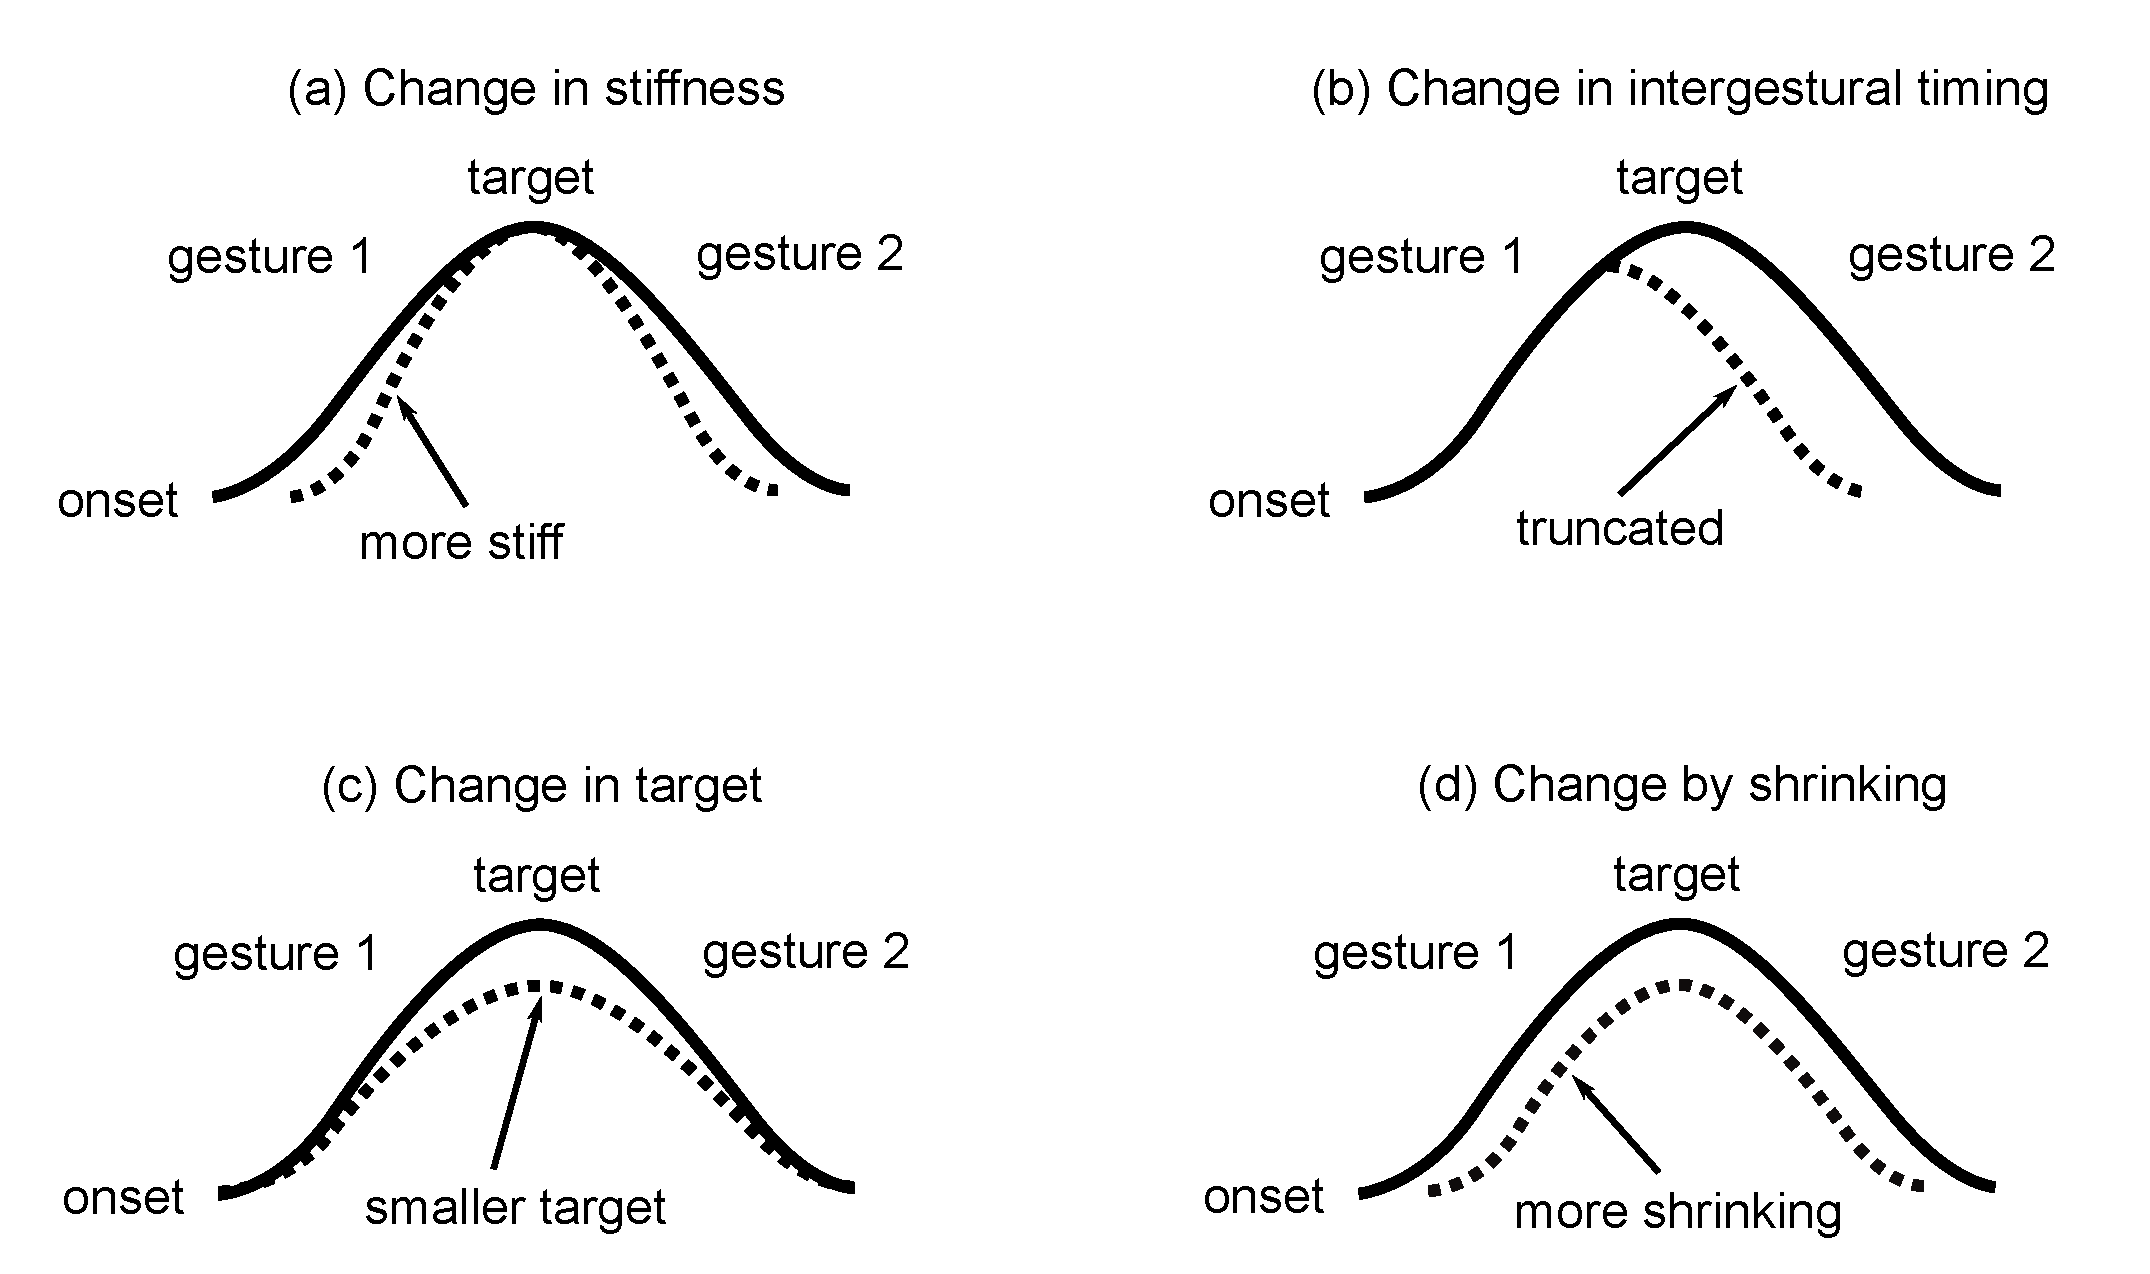
\includegraphics[width=\textwidth]{figures/ch4/cho_modifications.pdf}
\caption{Modifications of articulatory gestures induced by prominence following \citet{Cho2006}.}
\label{fig:cho_2006}
\end{figure}

The effect of prosodic structure on articulation, resulting in the modification of gestures as shown above, can be modelled using \emph{prosodic gestures}. Prosodic gestures are conceptualised as special gestures without any constriction. They exert control on the individual gestures responsible for the constrictions to produce vowels and consonants. This approach was developed to account for the fact that gestures are executed slower and overlap less in time at prosodic boundaries \citep{Byrd2000, ChoKeating2001, Fougeron2001, Tabain2003, Cho2006, KrivokapicByrd2012}. The proposal of \citet{Byrdetal2000} and \citet{ByrdSaltzman2003} is a prosodic gesture, called $\pi$-gesture, that modulates the intergestural timing at prosodic boundaries by modifying the stiffness of the constriction gestures co-activated with it. The extent to which the ``local speaking rate", i.e. the stiffness of gestures, is affected depends on the strength of the $\pi$-gesture \citep[13]{Byrd2000}. The activation level of the $\pi$-gesture is defined by the rank of the constituent in the prosodic strength.

While the $\pi$-gesture models what happens at prosodic boundaries, the $\mu$-ges\-ture has been developed to account for the modifications of articulatory gestures under prominence. Initially proposed to account for the effect of stress \citep{Saltzmanetal2008}, it comes in two different versions. The $\mu_T$-gesture is slows down the constriction gestures in the interval of activation like the $\pi$-gesture \citep{Krivokapic2014}. The $\mu_S$-gesture modulates the spatial properties of the constriction gestures. Although developed for stress, $\mu_S$-gestures can be applied to the level of accent as well.

\section{Prosodic focus marking beyond tone}
\label{sec:focus3}

With regard to focus structure, the results of \citet{MückeGrice2014} give interesting insights into how speakers use the modification of supra-laryngeal articulation. The study used the same data set as \citet{Griceetal2017} with the three focus types broad, narrow and contrastive focus. In addition, the data set contains material of a fourth condition in which the target word is in the background, i.e. out-of-focus. This condition corresponds to example \ref{ex:background}. Remember that in this condition the target word does not receive an accent. 

All target words in this data set are disyllabic with stress on the first syllable that is either /bi:/, /ba:/ or /bo:/. The authors measured the duration and the displacement of the opening gesture of the lips from the maximal constriction of the lips for the bilabial stop to the maximal opening for the vowel.

The data of \citet{MückeGrice2014} show that there is a gradual increase in the duration and displacement of the opening gesture from background to contrastive focus with intermediate values for broad and narrow focus, see Figure \ref{fig:muecke_grice_2014}. Interestingly, there does not seem to be a big step between background and broad focus, i.e. between unaccented and accented. In fact, \citet{MückeGrice2014} find a statistically significant effect between the two conditions for only one speaker (F1). In contrast to this finding, the modifications between broad focus and contrastive focus seem to be much larger. 

\begin{figure}
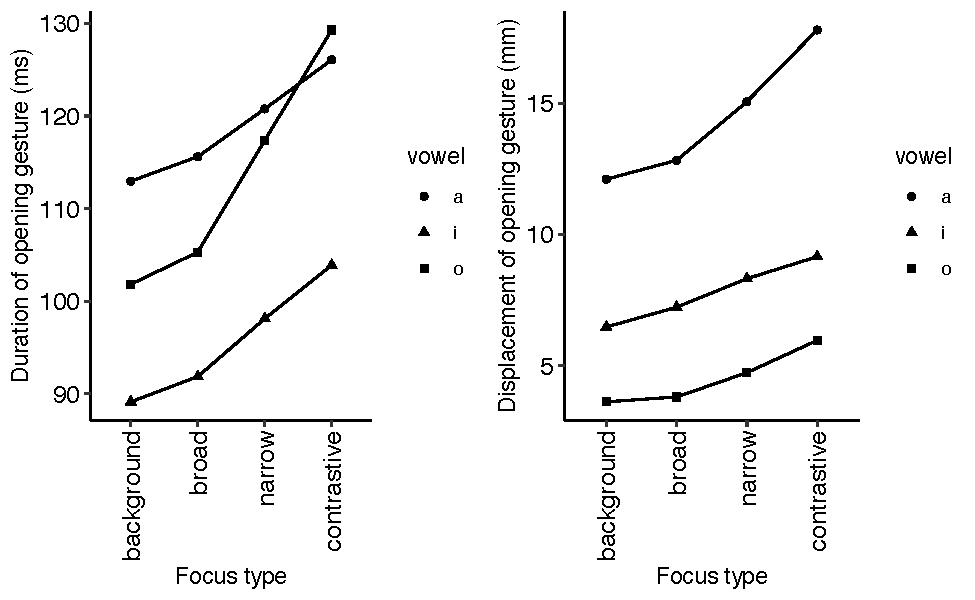
\includegraphics[width=\textwidth]{figures/ch4/muecke_grice_2014.pdf}
\caption{Mean duration and displacement of the vocalic opening gesture of the lips in the stressed syllable from the study of \citet{MückeGrice2014}.}
\label{fig:muecke_grice_2014}
\end{figure}

These data suggest that accented words do not necessarily have to be articulated differently from unaccented words (at least in the investigated articulatory dimensions). In addition, modifications of the supra-laryngeal articulation are used to encode focus structures that have the nuclear pitch accent in the same place (broad, narrow and contrastive focus all have the nuclear pitch accent on the target word). The latter result aligns well with the findings of \citet{Griceetal2017} that show tendencies to enhance prosodic prominence by choice of pitch accent type and the phonetic parameters of the pitch accent (alignment, onglide) from broad to narrow focus and from narrow to contrastive focus. It indicates that placing a nuclear pitch accent on a word is not the only important mechanism and that prominence is marked beyond accentuation. In addition to the categorical property of accentuation, continuous modulations play a significant role in the supra-laryngeal as well as the laryngeal system. These observations provide strong support for a view that acknowledges the importance of categoriality and continuity in prosody.

\section{Summary}
\label{sec:summary_prosody}

This chapter has been a whirlwind exploration of important concepts of prosody, prosodic structure and prosodic prominence. It has reviewed arguments for why it is reasonable to consider prosody as shaped by both categorical and continuous traits. The prosodic expression of focus was considered from different perspectives as focus is one of the most important functions of prosody in West-Germanic intonation languages. In addition, studies dealing with the prosodic marking of focus have revealed interesting results concerning the categorical and continuous aspects of prosody and their integration. The data presented in the following chapters of this book will also concentrate on focus and take the studies of \citet{MückeGrice2014} and \citet{Griceetal2017} as a basis for the experimental design, attempting to advance their conclusions by providing a formal modelling account.



  
%\chapter{Data collection: a controlled corpus of prosodic focus marking}
\label{chapter_data}

Forming the second part of the book, the next few chapters are concerned with a study on prosodic prominence in German that is designed to explore integration in a two-fold manner: First, it concentrates on the intertwining of categorical and continuous aspects of prosodic prominence. Second, it takes into account aspects of tonal structure as well as supra-laryngeal articulation, since both have been shown to be relevant for prosodic prominence in Chapter \ref{chapter_prosody}. Special attention is going to be paid to the theoretical implications that the data reveal. Therefore, a major part of this second part of the book is going to be concerned with the development of a model that is able to explain categoriality and continuity as the outcome of a single system. This model owes a lot to the dynamical models presented in Chapter \ref{chapter_ds} and aims to contribute to a theoretical symbiosis of the categorical and the continuous aspects of speech. This symbiosis can be stated more concretely in viewing phonetics and phonology as a unified system in which ``a single formal language, nonlinear dynamics, makes it possible to model the relation between the discreteness of phonological form and the continuity of phonetic substance" \citep[937]{GafosBenus2006}. 

Building on the studies of \citet{MückeGrice2014} and \citet{Griceetal2017}, the current work investigates the expression of focus by prosodic means in a controlled laboratory setting. A large data pool was elicited that allows extensive examinations of the interplay of categorical and continuous aspects of prosodic focus marking and prosodic prominence. The following chapters describe the results obtained from the various analyses performed on the corpus and the modelling approaches designed to capture the main generalisations that the data provides for linguistic theory. Both chapters make use of the same data set, or subsets of the same data set, and employ similar measurement methods. These methods are explained in the current chapter. But before turning to the methodology, the research goals of the present study shall be stated more clearly. 

The aims pursued by the research presented in this second part of the present work can be formulated as follows: First, it will be investigated whether the relation of nuclear pitch accent type to focus type can be described as one-to-one or whether the mapping can best be characterised as fuzzy and probabilistic with different proportions of pitch accent types present in each focus type. Second, in addition to tendencies of the use of categories to differentiate focus types -- even if their distributions might not be clear-cut or non-overlapping -- the continuous aspects of the realisation of the pitch accent types will be investigated. Third, it will be examined whether there is co-variation of categorical and continuous aspects of the pitch accent patterns found in the data. Fourth, as stated above, the study will take a look beyond F0 and investigate the supra-laryngeal modifications (tongue and lip kinematics) used to express prominence and mark focus types. In this context, modifications found between unaccented and accented words as well as modifications within the group of accented words in different focus types will be considered. This last research goal is suited to contribute to our understanding of the interplay between categories and continuous modifications. Since \emph{accentuation} is conceptualised as a categorical quality of prosodic structure, it is interesting to consider whether articulatory modifications mirror this categorical nature or whether articulatory modifications are used in a continuous way to enhance prosodic prominence beyond accentuation. Furthermore, including tonal and articulatory aspects in the analysis has the potential to advance our understanding of the multiple dimensions that are recruited to express prosodic prominence.

\section{Speakers and recordings}

Twenty-seven monolingual German native speakers were recorded acoustically using a head-mounted condenser microphone and with 3D Electromagnetic Articulography (EMA) using a Carstens AG501 articulograph. The acoustic recordings were carried out with an AKG C520 headset microphone into a computer via a PreSonus AudioBox 22 VSL interface at a sampling rate of 44.1 kHz and a bit depth of 16 bit. For the EMA recordings, sensors were placed on the jaw, upper and lower lip, tongue tip, tongue blade, and tongue body to track the movements of the articulators. To compensate for head movements, reference sensors were placed on the bridge of the nose and behind the ears. A bite plate measure was used to rotate the occlusal plane. The articulatory data were recorded at 1,250 Hz, downsampled to 250 Hz and smoothed with a 3-step floating mean. In this work, the data from the lip sensors and the backmost tongue sensor are analysed.

All recordings took place at the I\emph{f}L -- Phonetik department of the University of Cologne. The speakers were aged between 19 and 35 at the time of recording. 17 of them were female, 10 were male. None of the subjects had a special training in phonetics, phonology or prosody, or reported any speech or hearing impairments. The participants received compensation for their participation in the study. The recording session, after the participant had been prepared, lasted about 45 minutes including a training session.

The participants were involved in an interactive animated game sitting in front of a computer screen. They were told that the game revolved around two robots working in a factory. One of the robots likes to move around the tools while the other, slightly older and technologically outdated, needs the participant's help to retrieve these tools. In each trial, the participant first saw one robot placing the tool on an object in the factory room and leaving the scene. In the next step, the second, older robot entered the scene. This robot did not enter the factory room but stopped in front of the closed door asking a question about the action of the first robot. After the participant's answer, the door opened and the second robot entered the room, took the tool, and left the scene.

\section{Speech material}

Natural productions by a male, native German speaker were used for the robot's questions that served as triggers for the focus structures of the answers. They were chosen such that the target word denoting the object (where the tool is placed) could be in broad focus, narrow focus, contrastive focus, or in background (with a contrastive focus on the direct object). 

Table \ref{tab:focus_trigger_target} shows examples for such question-answer-pairs. In the examples, square brackets and subscript $F$ mark the focus domain. Each question was given auditorily and additionally shown as a combination of pictures in a thought bubble above the robot's head: the question tool on top of the question object in the case of background and contrastive focus; a simple question mark in the case of broad focus; the object and the question word ``wo?" (`where?') in the case of narrow focus. The answers that the participant had to produce were presented in written form at the bottom of the screen. Many participants reported that they were able to give the answers without reading them on the screen after some trials. The participants were asked to always produce the answer with the same syntactic structure and to not add any words like ``nein" (`no'). None of the participants had any problems with this restriction. Likewise, none of the participants reported that they found the sentences unnatural or difficult.

\begin{table}
\caption{Example question-answer-pairs to elicit the focus structures.}
\label{tab:focus_trigger_target}
\begin{tabularx}{\textwidth}{l Q}
	\lsptoprule
Focus structure & Example trigger (Q) and target sentence (A) \\
\midrule
Background & Q: Hat er die Säge auf die Wohse gelegt? \\
& \hspace{5 mm}`Did he put the saw on the Wohse?' \\
& A: Er hat [den Hammer]$_F$ auf die Wohse gelegt. \\
& \hspace{5 mm}`He put the hammer on the Wohse.'\\
& \\
Broad focus & Q: Was hat er gemacht? \\
& \hspace{5 mm}`What did he do?' \\
& A: Er hat [den Hammer auf die Wohse gelegt.]$_F$ \\
& \hspace{5 mm}`He put the hammer on the Wohse.' \\
& \\
Narrow focus & Q: Wo hat er den Hammer hingelegt? \\
& \hspace{5 mm}`Where did he put the hammer?' \\
& A: Er hat den Hammer [auf die Wohse]$_F$ gelegt. \\
& \hspace{5 mm}`He put the hammer on the Wohse.' \\
& \\
Contrastive focus & Q: Hat er den Hammer auf die Mahse gelegt? \\
& \hspace{5 mm}`Did he put the hammer on the Mahse?' \\
& A: Er hat den Hammer auf [die Wohse]$_F$ gelegt. \\
& \hspace{5 mm}`He put the hammer on the Wohse.'\\
\lspbottomrule
\end{tabularx}
\end{table}

To control for the segmental context and for word frequency, twenty German sounding disyllabic nonce words with a C$_1$V$_1$:C$_2$ǝ structure were chosen as target words. The words were designed to have word stress on the first syllable. The stressed vowel V$_1$ was either /a:/ or /o:/, the second vowel always schwa. The consonants (C$_1$ and C$_2$) either require movements of the labial system or the tongue tip to avoid influences on the tongue body measures for the vowel. The first consonant was chosen from the set of /n m b l v/, the second consonant from /n m z l v/. The consonants and vowels were combined such that each first consonant C$_1$ of /n m b l v/ occurred twice with each first vowel V$_1$ /a:/ or /o:/. Each second consonant-schwa-combination /nǝ mǝ zǝ lǝ vǝ/ occurred four times in the whole set. Special care was taken that the words did not overlap with real German words. All words were presented with the female determiner ``die" /di:/. All participants pronounced the words as expected. The target words are listed in Table \ref{tab:target_words}.

\begin{table}
\caption{Target words.}
\begin{tabularx}{\textwidth}{XXXXl}
\lsptoprule
Nohme & Mohme & Bohme & Lohne & Wohme \\ 
Nohse & Mohwe & Bohwe & Lohle & Wohse \\ 
Nahne & Mahne & Bahle & Lahse & Wahne \\ 
Nahle & Mahse & Bahwe & Lahle & Wahwe\\
\lspbottomrule
\end{tabularx}
\label{tab:target_words}
\end{table}

In the setting of the experiment, each target word was associated with a fictitious visual object. The association remained fixed throughout the whole experiment and across all participants. There was no connection between the appearance of the object and the sound of the word. The participants were presented with all objects and target words in a preparation phase immediately before the experiment and were asked to read the words aloud with the determiner ``die" (``die Nohme", ``die Lahse", etc.). This phase lasted a few minutes and was included to ensure that no participant placed the stress on the second syllable or had any difficulties pronouncing the words. All participants placed word stress on the first syllable starting with the first production.

As described above, in each trial, a tool is placed on one of the fictitious objects. Each object was paired with a tool to occur with. All tools are given in Table \ref{tab:tools}. Since there were 10 tools and 20 target words in the game, each tool had to occur twice. Furthermore, for the background condition and the contrastive focus condition, a competitor tool or object was needed: for the direct object of the question when the target word was in the background (``Did he place X on A?” “He placed Y on A!”) and for the indirect object of the question when the target word was in contrastive focus (``Did he place X on A?” “He placed X on B!"). These combinations were fixed for all participants, yielding 20 quadruples of target object, tool, competitor object, and competitor tool.\footnote{In the case of trials with broad focus or narrow focus, the competitor object and the competitor tool are not needed. Thus, in the quadruples for broad and narrow focus trials, these positions are empty.} The competitor object was chosen randomly with the restriction that the first consonant or the first vowel did not equal the first vowel or consonant of the target object. The competitor tool was selected such that it differed in the first consonant from the target sentence tool. The 20 target words occurred with all four focus conditions resulting in 80 trials per speaker. As a training phase, 16 trials with different objects and tools (everyday objects, e.g. a table) preceded the actual experiment session. 

\begin{table}
\caption{Tools with English translation.}
\begin{tabularx}{\textwidth}{XlXl}
	\lsptoprule
\textbf{Tool} & \textbf{Translation} & \textbf{Tool} & \textbf{Translation} \\
\hline
Amboss & anvil & Pinsel & Paint brush \\
Besen & broom & Rolle & Paint roller \\ 
Bohrer & drill & Säge & Saw \\
Bürste & brush & Schere & Scissors \\
Hammer & Hammer Zange & Pliers\\
 \lspbottomrule
\end{tabularx}
\label{tab:tools}
\end{table}

For each of the 27 participants the order of trials was randomised with some restrictions: Subsequent trials were not allowed to contain the same target word or tool used in the target sentence. Furthermore, there were no three subsequent trials with the same focus condition. For two subsequent trials with identical focus condition an upper limit was set: In only 15\% of the list, two adjacent trials with equal focus conditions occurred.

The scenes, objects, tools, and robots were drawn by a professional book illustrator. The game was developed as an interactive website using HTML and JavaScript with jQuery for animation (e.g. robots' arm and mouth movement, the door opening, and closing). The experimenter sat behind the participant and pressed a key on the keyboard to make the robot move toward the tool and proceed to the next trial. There was a ``rescue key" to repeat the trial in case something went wrong. Between trials, the scenery disappeared for 4 seconds and the screen transitioned through a series of light, muted colours. This short break detached the trials from one another to make sure that the focus structure of the target sentence made reference to the current trial only and not to the previous trial. In order to make the task more game-like, points were counted for each complete trial in the lower right corner of the screen. Figure \ref{fig:exp_trial} presents an example of the experiment screen where the second robot has just asked his question and is waiting for the answer of the participant. The code of the experiment app is available under open source and creative commons license: \href{http://doi.org/10.5281/zenodo.2611287}{http://doi.org/10.5281/zenodo.2611287}.

\begin{figure}
\fbox{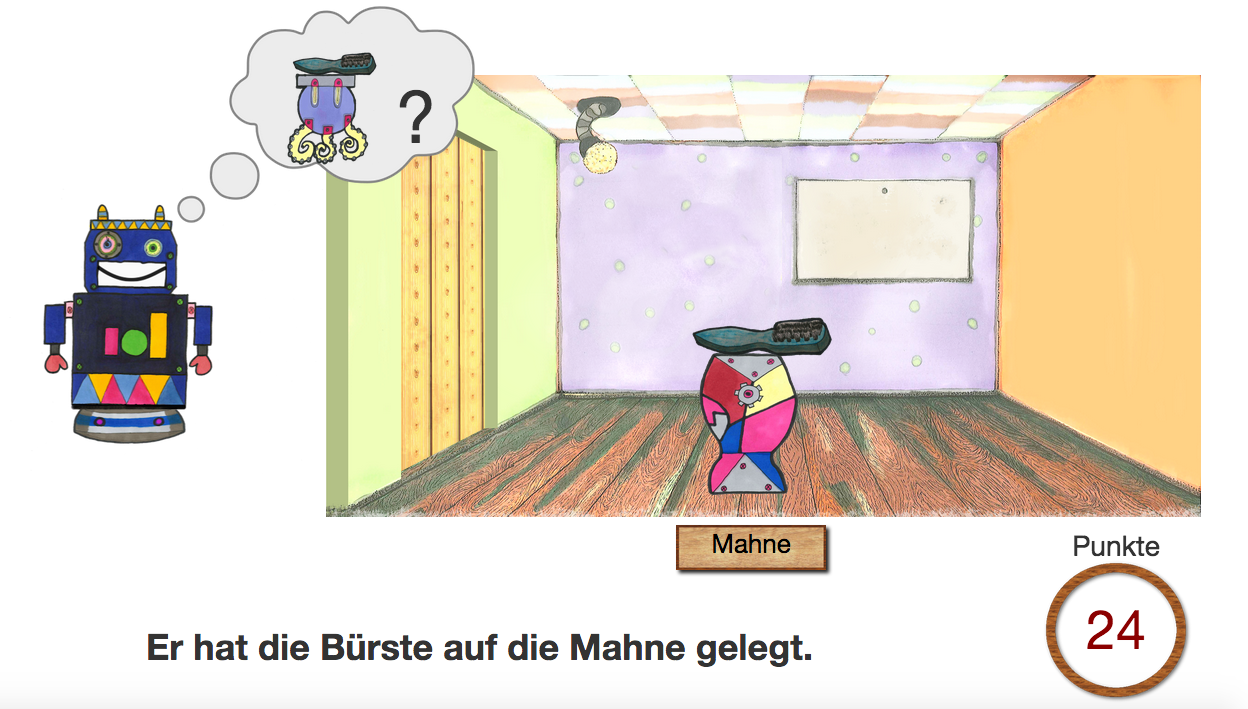
\includegraphics[width=.95\textwidth]{figures/ch5/Exp_Trial.png}}
\caption{Example screen from the experiment during a trial with contrastive focus condition.}
\label{fig:exp_trial}
\end{figure}

\section{Measures}

This section describes the various measures performed on the data set. All measures are in some form based on the annotation of the stressed syllable and the vowel of the stressed syllable. One trained annotator labelled the beginning and end of the stressed syllable of each target word using the waveform and the spectrogram in the emuR speech database system \citep{Winkelmannetal2018}. Another trained annotator labelled the beginning of the vowel of this syllable in Praat \citep{BoersmaWeenink2018}. 

\subsection{Tonal onglide}

To assess the differences in the F0 contours, the tonal onglide of each nuclear pitch accent was measured. Figure \ref{fig:onglide_measure} provides a schematic depiction of the tonal onglide measure. The tonal onglide characterises the portion of the F0 movement towards the main tonal target of the pitch accent \citep{RitterGrice2015}. In terms of an autosegmental-metrical analysis, like GToBI \citep{GriceBaumannBenzmüller2005}, L+H* and H* pitch accent types are described by a rising movement and result in positive onglide values. In contrast, the accent types H+L* or H+!H* are described by a falling movement from the initial high portion of the accent down to the L* or !H* on the accented syllable and result in negative onglide values. In addition to capturing the direction of the tonal movement (``is it rising or falling?"), the tonal onglide reflects the magnitude of the rise or fall in semitones (``how much does it rise or fall?"). Albeit being a continuous variable that represents both the direction of the pitch movement as well as the magnitude of this movement, the tonal onglide does not capture all relevant details of pitch accents \citep{Griceetal2017}. Nevertheless, it has been shown that the tonal onglide movement is a perceptually relevant parameter of pitch accents in German \citep{BaumannRöhr2015, RitterGrice2015}.

F0 movements were annotated by two labellers with training in prosody using a simple labelling scheme without having access to the intended focus structures of the sentences. First, the labellers identified all utterances in which the speaker did not place the nuclear pitch accent on the object. Only cases which exhibited a clear nuclear accent on the target word for both annotators were labelled as accented. Second, the labellers judged perceptually whether the nuclear pitch accent was falling or rising. Third, the labellers identified the beginning and the end of the onglide movement manually within a window of three syllables including the accented syllable in the centre, the syllable before and the syllable after the accented syllable.

For rising accents, a local minimum just before the rising movement was annotated in the pre-accented syllable or the accented syllable itself as the beginning of the onglide movement. A local maximum at the end of the rise was labelled in the accented syllable or the post-accented syllable as the end of the movement. For falling accents, a relatively high point at the start of the fall was labelled in the pre-accented syllable or the accented syllable itself as the beginning of the onglide movement. Since F0 is usually falling throughout the syllable in a falling accent and hence a tonal target is virtually impossible to determine, the midpoint of the vowel of the accented syllable was marked as the end of the accentual movement.

If the nuclear accent was not placed on the target word, it was placed on the direct object of the sentence. In this case, the part of the phrase containing the target word and the following verb is characterised by a low stretch of F0. This situation -- deaccentuation of the target word -- was found in almost all cases of the background condition and in a minority of cases of the other conditions. When deaccentuation of the target word occurred, an ``onglide” measure was carried out with fixed time points (5 ms before the start and 50 ms before the end of the stressed syllable). It is not possible to speak of tonal onglide in a strict sense here since there is no tonal movement of a pitch accent. Hence, there is no beginning and end of a tonal movement that can be identified. However, this measure makes it possible to compare and model the intonation of all utterances, with accented and unaccented target words, and to relate the intonational and articulatory modifications used to express focus structure across all experimental conditions.

Although using the semitones scale already eliminates a great deal of variation between speakers, like gender effects, normalisation is needed to make the speakers more comparable. To do so, each rising onglide value is divided by the mean of the speaker’s rising onglides, and each falling onglide value is divided by the mean of the speaker’s falling onglides. It is plausible that a rise is best interpreted in relation to other rises, while a fall is best interpreted in relation to other falls of the same speaker. For example, a raw onglide value of +6 semitones might be quite extreme for a speaker with a mean of +4 semitones for rises compared to a speaker with a mean of +6 semitones for rises. For the unaccented cases, where it is not possible to speak of rises and falls, the overall mean of the absolute onglide values for each speaker was used in the normalisation procedure.

\begin{figure}
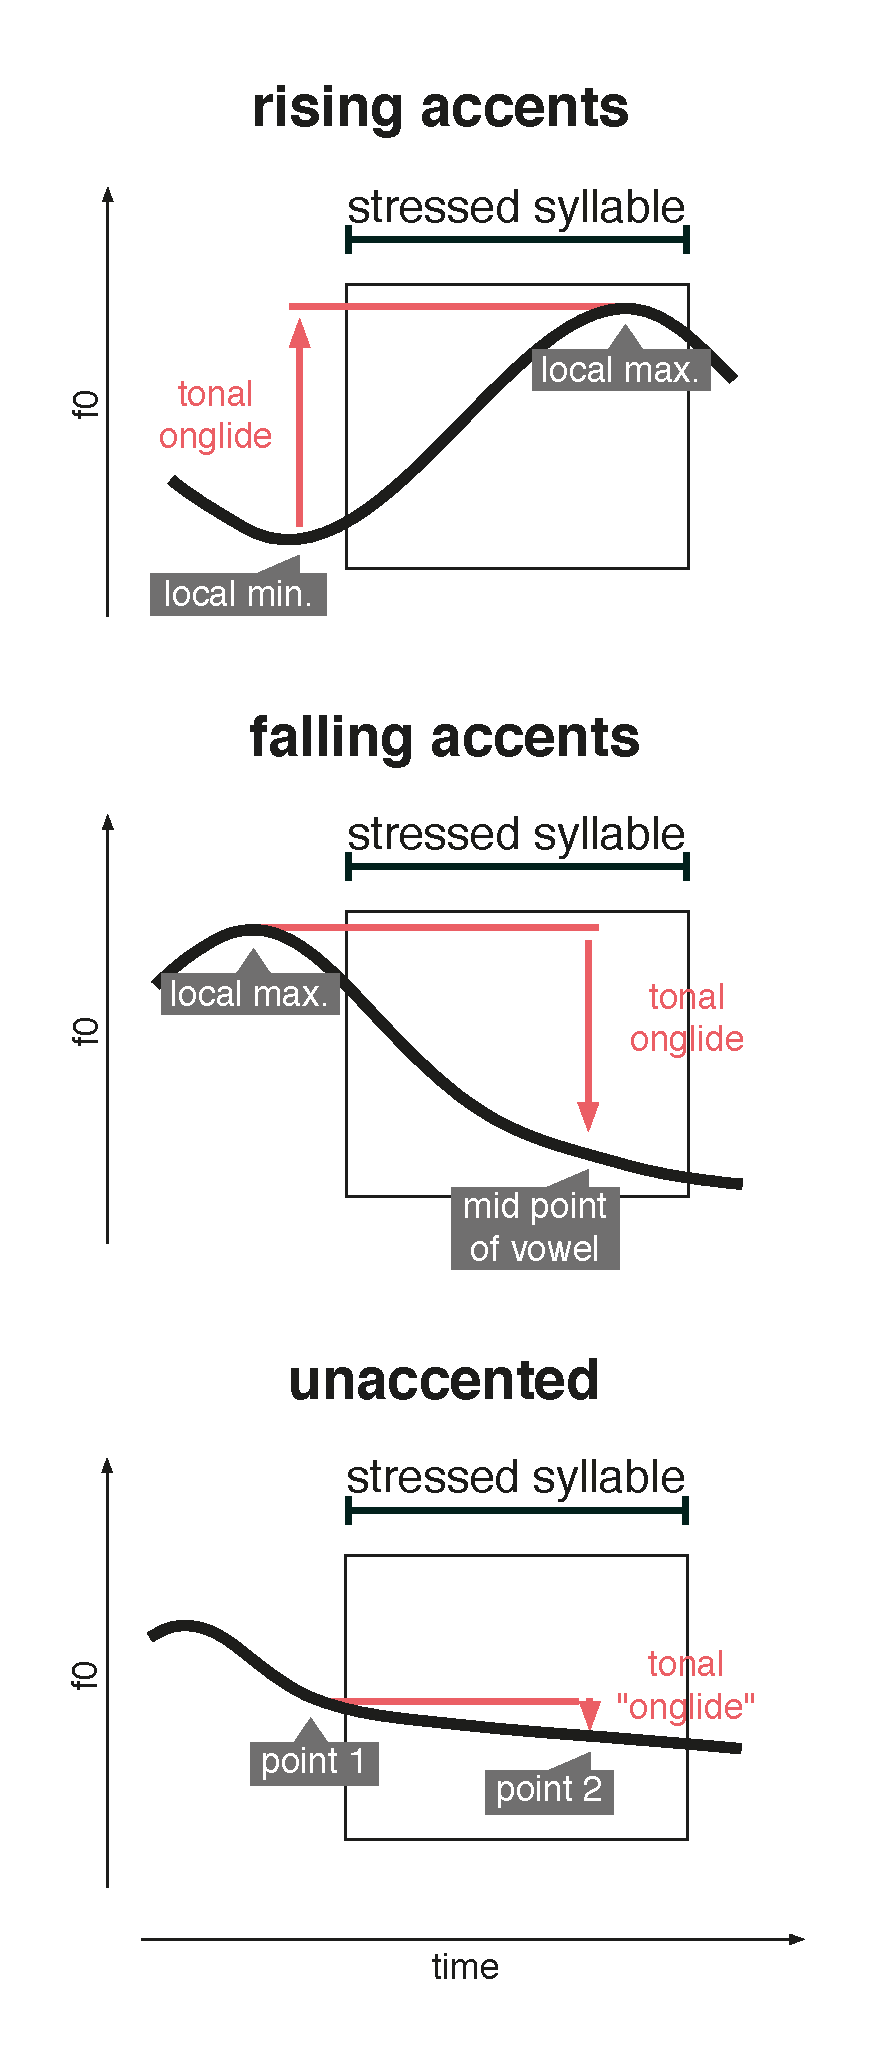
\includegraphics[width=7cm]{figures/ch5/measures_onglide.pdf}
\caption{Schema of tonal onglide measure.}
\label{fig:onglide_measure}
\end{figure}

\subsection{Alignment of the peak}

The labels described above for the tonal onglide were used to determine the alignment of the peak. In the case of falling accents, the beginning of the fall was used as the peak; in the case of rising accents, the end of the rise was used as the peak. The alignment of the peak is calculated as the difference between the time point of the peak and the time point of the beginning of the vowel in the accented syllable in ms. No equivalent for deaccented target words could be applied for this measure. Figure \ref{fig:alignment_measure} shows a schema of the measure.

\begin{figure}
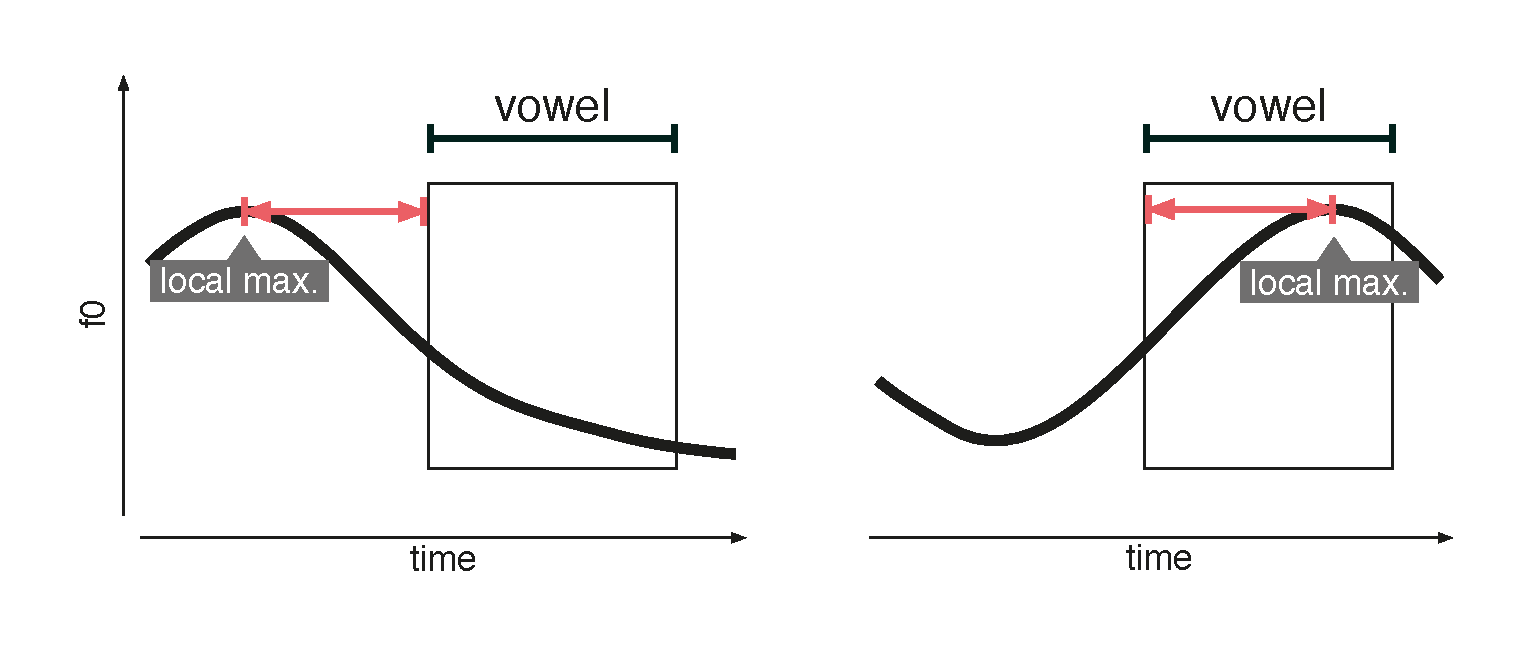
\includegraphics[width=\textwidth]{figures/ch5/measures_alignment.pdf}
\caption{Schema of alignment measure.}
\label{fig:alignment_measure}
\end{figure}

\subsection{Lip aperture}

Lip aperture was evaluated as the Euclidean distance between the lips, as given in Equation \ref{eq:eukl_lips} \citep{Byrd2000}, within the boundaries of the syllable. An automatic procedure was used to determine the maximum of the trajectory within the boundaries of the labelled acoustic syllable. The maximal lip aperture represents the widest opening of the lips during the production of the vowel. Figure \ref{fig:lip_measure} presents a schema of this measure.

\begin{equation}
\begin{split}
\text{lip aperture } x &= \text{upper lip } x - \text{lower lip } x\\
\text{lip aperture } y &= \text{upper lip } y - \text{lower lip } y\\
\text{lip aperture} &= \sqrt{(\text{lip aperture } x)^2+(\text{lip aperture } y)^2}
\end{split}
\label{eq:eukl_lips}
\end{equation}

\begin{figure}
\includegraphics[width=7cm]{figures/ch5/measures_lips.pdf}
\caption{Schema of the lip aperture measure.}
\label{fig:lip_measure}
\end{figure}

\subsection{Position of the tongue body}

The vertical (high-low) and the horizontal (front-back) position of the back-most tongue sensor was measured as an indication of the position of the tongue body. Because the stressed syllable is followed by a syllable containing schwa, the exact target of the horizontal tongue body movement could not consistently be determined for the vowel /o/ in the stressed syllable as schwa can be lower than /o/. Therefore, a different method was applied for all tongue trajectory measures: The first 50\% of each acoustic vowel was taken as a time window to measure the tongue body position. The mean of all points on the trajectory falling in this 50\% window was calculated for each token. The length of the window (50\%) is, of course, arbitrary. However, it seems plausible to assume that the acoustic vowel is a perceptually relevant time interval. It thus makes sense to ask how high or low, back or front the vowel is articulated in this window. Using only the first 50\% reduces the influence of the following vowel on the measure. Figure \ref{fig:tounge_measure} shows a schema of the measure for two different trajectories and the potential outcome of the measure (as bar graphs). The measure was used on both the horizontal and the vertical dimension of the movement as well as for both vowels /a/ and /o/ to make all measures comparable.

\begin{figure}
\includegraphics[width=\textwidth]{figures/ch5/measures_tbo2.pdf}
\caption{Schema of the tongue body measure.}
\label{fig:tounge_measure}
\end{figure}

\section{Data and availability}

Of the 2160 planned utterances (80 utterances per speaker, 27 speakers), 29 (1.3\%) productions had to be excluded due to technical problems during the recording or because the participant did not pronounce the words of the sentence correctly (and the trial was not repeated). The total dataset comprised 2131 recordings. 

As stated above, the target word is unaccented in the background condition in the majority of cases. Conversely, the target word is accented in the majority of cases in all other conditions (broad focus, narrow focus, and contrastive focus). This situation was expected and planned in the design of the study (see Chapter \ref{chapter_prosody}). The opposition background vs. \{broad focus, narrow focus, contrastive focus\} is used for the comparison of unaccented and accented. Therefore, all tokens with accented target words are excluded from the background condition (0.14\% of the productions in the complete corpus of 2131 utterances). Likewise, all tokens with unaccented target words are excluded from the conditions broad focus, narrow focus and contrastive focus (1.88\% of the productions in the complete corpus of 2131 utterances). It has to be noted that only those cases were labelled as accented that exhibited a clear nuclear pitch accent on the target word for both annotators. All in all, 2088 utterances enter the analysis, i.e. 96.67\% of the 2160 planned utterances. The data set is accessible for download: \href{https://osf.io/4g6s2/}{https://osf.io/4g6s2/}.

 
%\chapter{Integrating categorical and continuous aspects of pitch accents}
\label{chapter_onglide_modelling}

The first analysis of the controlled corpus of prosodic focus marking is concerned with intonation contours, more specifically with nuclear pitch accents. The results outlined in this chapter show that parameters of pitch accents are used in a categorical as well as a continuous manner at the same time. The two kinds of using F0 modulations seem to be applied by speakers to achieve the same -- or at least comparable -- communicative ends. This striking parallel is implemented in a first sketch of a dynamical model. The model conceptualises pitch accents as attractors in a continuous phase space. In doing so, it is able to capture the categorical nature of pitch accents, continuous variation within one pitch accent category and the generalisation that the categorical and the continuous use of intonation are related. In addition, two subgroups of speakers are identified that exhibit different patterns of intonational focus marking. Despite their differences, the behaviour of both groups can be described by means of the same model.

\section{Results of F0 measures}

As outlined in Chapter \ref{chapter_data}, the nuclear pitch accents in the corpus are assessed using two continuous parameters: tonal onglide and alignment of the peak. This section outlines the results of the two measures. Since the present chapter deals with nuclear accents only, the background condition is not included in the analyses since the vast majority (99\%) of target words in the background condition were unaccented. A treatment of this condition is added to the analysis in the next chapter (Chapter \ref{chapter_multi_prosody}).

\subsection{Tonal onglide}

Before turning to the results of the tonal onglide, it is useful to consider some example contours from the corpus. Gaining an impressionistic perspective of the data is particularly helpful in discussing tonal onglide since this measure is far less established in the research literature than the alignment of the peak. Figure \ref{fig:example_contours} presents one instance of broad (top), narrow (middle) and contrastive focus (bottom) each produced by male speaker. The stressed syllable of the target word is marked by the blue box, the arrows illustrate the F0 movement that is captured by the tonal onglide measure. The informative value of these examples is of course limited since they only represent individual utterances. However, accompanying the quantitative results, they help to give a thorough insight into the data. The figure shows that the speaker uses a falling accent in broad focus and rising accents in narrow focus and contrastive focus. Comparing these last two conditions, a larger magnitude of the rise can be attested in contrastive focus. As the following quantitative results show, this first impression is supported by the data set but there is more variation involved. 

\begin{figure}[t]
\includegraphics[width=\textwidth]{figures/ch6/intonation_contours.pdf}
\caption[Examples of intonation contours for broad, narrow, and contrastive focus.]{Example intonation contours for broad (top), narrow (middle), and contrastive focus (bottom). The blue box marks the nuclear accented syllable. The red arrows indicate the direction of the tonal onglide.}
\label{fig:example_contours}
\end{figure}

Figure \ref{fig:onglide_distributions_within} plots the distributions of normalised onglide values of all speakers together for broad focus, narrow focus and contrastive focus. Note that negative onglides indicate a falling tonal movement while positive onglides indicate a rising tonal movement. Broad focus is characterised by an almost symmetrical bimodal distribution, reflecting the fact that both falling and rising accents are equally possible in this focus condition. Moving on to narrow focus, the right mode of the distribution grows, indicating that the majority of accents are rising in this condition. This trend is continued in contrastive focus for which an even higher proportion of rising accents is found. The numbers and proportions of falling and rising onglides are summarised in Table \ref{tab:props_onglide}. In a minority of cases (6 cases, 0.38\% of the data), it was not possible to track the F0 at the locations marked by the labellers, rendering the onglide measure impossible to apply (labelled ``NA" in the table). 

The distributions reveal that there is no one-to-one mapping of accent type (rising/falling) to focus type, a finding that is in line with the literature. Rather, a probabilistic mapping of accent type to focus type with a large degree of overlap can be attested. Figure \ref{fig:onglide_means} provides a closer look at the rising portions of all three distributions. In addition to the increase in the proportion of rising accents, the rises themselves tend to become larger in magnitude. 

\begin{figure}
\includegraphics[width=\textwidth]{figures/ch6/onglide_norm_distribution_within.pdf}
\caption{Distributions of normalised tonal onglide values for broad, narrow and contrastive focus.}
\label{fig:onglide_distributions_within}
\end{figure}

\begin{table}
\caption{Proportions of falling and rising onglides.}
\begin{tabularx}{\textwidth}{Xllll}
	\lsptoprule
\textbf{focus types	} &	\textbf{falling accents}&		\textbf{rising accents} &			\textbf{NA} & 	\textbf{all}\\
&				\textbf{(negative onglides)} &	\textbf{(positive onglides)} &		&			\\	
\midrule
broad focus &		241 (47.07\%) & 				270 (52.73\%)  & 					1 (0.2\%) &			512 \\
%&				47.07\% &				52.73\% &					0.2\% &		\\
\midrule
narrow focus &		115 (21.78\%)  &				411 (77.84\%) & 					2 (0.38\%)  &			528 \\
%&				21.78\% &				77.84\% & 					0.38\% &		\\
\midrule
contrastive focus &		47 (9.04\%)  &					470 (90.38\%) &						3 (0.58\%) &			520 \\
%&				9.04\% &				90.38\% &					0.58\% &		\\
\midrule
all &				403 (25.83\%) &					1151 (73.78\%)  &					6 (0.38\%) &			1560\\\lspbottomrule
%&				25.83\% & 				73.78\% &					0.38\% & 		\\ \lspbottomrule\lspbottomrule
\end{tabularx}
\label{tab:props_onglide}
\end{table}%

\begin{figure}
\includegraphics[width=7.5cm]{figures/ch6/onglide_norm_rising_means.pdf}
\caption{Means of rising onglides (normalised) for broad, narrow and contrastive focus.}
\label{fig:onglide_means}
\end{figure}

The results are analysed using a Bayesian linear mixed model in R \citep{RCoreTeam2018} with the package brms \citep{Buerkner2018} which implements an interface to Bayesian inference with MCMC sampling in Stan \citep{Carpenteretal2017}. The estimated differences between focus conditions in terms of posterior means are reported in addition to 95\% credible intervals, and the probability of the estimate being greater than zero. Given the data and the model, the 95\% credible intervals indicate the range in which one can be certain with a probability of 0.95 that the difference between estimates can be found. To calculate the differences between focus types,  the analysis subtracts the posterior samples for background from broad focus (broad–background), broad focus from narrow focus (narrow–broad), narrow focus from contrastive focus (contrastive–narrow), and broad focus from contrastive focus (contrastive–broad).

Normalised onglide is included as the dependent variable in the model, focus type as a fixed effect, and random intercepts for speakers and target words as well as by-speaker slopes for the effect of focus type. Since the distribution of the dependent variable is bimodal, a prior for the predictor is used that is characterised by a mixture of two Gaussian distributions centred around −0.5 and 0.5 respectively. The model estimates the parameter theta that represents the extent to which the two Gaussian distributions are mixed. This parameter is referred to as the mixing parameter. For this parameter, a prior centred around zero is used. Differences in the mixing parameter indicate differences in the proportions of the two modes in the onglide data. The model runs with four sampling chains of 3,000 iterations each.

The presentation of the results starts with the mixing parameter. Given the model and the data, the analysis yields evidence for differences in the posterior probabilities for the mixing parameter between broad focus and narrow focus ($\hat\beta=1.32, CI=[0.60, 1.95], \allowbreak Pr(\hat\beta>0)=1$), narrow focus and contrastive focus ($\hat\beta=1.59, CI=[0.56, 2.65], \allowbreak Pr(\hat\beta>0)=1$) as well as broad focus and contrastive focus ($\hat\beta=2.91, CI=[1.61, 4.09], \allowbreak Pr(\hat\beta>0)=1$).

To assess the differences between the focus conditions regarding the rising distributions, the mean estimates of the right Gaussian sub-distribution are investigated. Given the model and the data, the analysis yields evidence for differences in the posterior probabilities for the mixing parameter between broad focus and narrow focus ($\hat\beta=0.14, CI=[0.07, 0.20], \allowbreak Pr(\hat\beta>0)=1$), narrow focus and contrastive focus ($\hat\beta=0.24, CI=[0.16, 0.32], \allowbreak Pr(\hat\beta>0)=1$) as well as broad focus and contrastive focus ($\hat\beta=0.37, CI=[0.30, 0.45], \allowbreak Pr(\hat\beta>0)=1$).

\subsection{Alignment of the peak}

In addition to the scaling of an accent -- an aspect that is captured by the tonal onglide -- the alignment of the peak has been reported to be an important dimension of pitch accents \citep[see also Chapter \ref{chapter_prosody}]{Gussenhoven2004, Ladd2008, LaddMorton1997}. The measure includes not only the peak alignment of rising accents but also the peak alignment of falling accents. This means that the peaks investigated here are of two kinds in terms of an autosegmental-metrical analysis: In rising accents, H* and L+H*, the peak belongs to the starred tone, for falling accents, H+!H* or H+L*, it belongs to the leading tone.

Negative alignment values indicate that the peak is early, i.e. before the onset of the vowel, while positive alignment values characterise a mid or late peak, i.e. after the vowel onset. The latter are referred to as \emph{mid to late peaks} in what follows. Figure \ref{fig:alignment_distributions_within} presents the distributions of alignment values of all speakers together for broad, narrow and contrastive focus. Similar to the distributions of the tonal onglide, the right mode increases in relation to the left mode when going from broad to narrow focus and from narrow to contrastive focus. The numbers and proportions of early and mid to late peaks are summarised in Table \ref{tab:props_alignment}. Note that the numbers of NA data points is different from the tonal onglide as the alignment measure is only based on the time points and not on the calculation of F0 that may fail due to technical issues in some cases.

Figure \ref{fig:alignment_means}\footnote{Note that the x-axis does not start at zero.} presents the means of the positive alignments (mid to late peaks) and shows that in addition to lower proportions of early peaks, the positive alignments increase, i.e. the instances within the group of mid to late peaks become later, although the difference between narrow and contrastive focus appears to be very subtle.

\begin{figure}
\includegraphics[width=\textwidth]{figures/ch6/alignment_distribution_within.pdf}
\caption{Distributions of alignment values for broad, narrow and contrastive focus.}
\label{fig:alignment_distributions_within}
\end{figure}

\begin{table}
\caption{Proportions of early and mid to late alignments.}
\begin{tabularx}{\textwidth}{Xllll}
	\lsptoprule
\textbf{focus types	} &	\textbf{early peak}&		\textbf{mid to late peak} &		\textbf{NA} & 	\textbf{all}\\
&				\textbf{(negative alignment)} &	\textbf{(positive alignment)} &		&			\\	
\midrule
broad focus &		241 (47.07\%) & 				271 (52.93\%)  & 					0 (0\%) &			512	\\
%&				47.07\% &				52.93\% &					0\% &			\\
\midrule
narrow focus &		117 (22.16\%)  &				411 (77.84\%) & 					0 (0\%)  &			528 \\
%&				22.16\% &				77.84\% & 					0\% &			\\
\midrule
contrastive focus &		47 (9.04\%)  &					473 (90.96\%) &						0 (0\%) &			520 \\
%&				9.04\% &				90.96\% &					0\% &			\\
\midrule
all &				405 (25.96\%) &					1155 (74.04\%)  &					0 (0\%) &			1560	\\\lspbottomrule
%&				25.96\% & 				74.04\% &					0\% & 		\\ \lspbottomrule
\end{tabularx}
\label{tab:props_alignment}
\end{table}%

\begin{figure}
\includegraphics[width=7.5cm]{figures/ch6/alignment_mid_late_means.pdf}
\caption{Means of positive alignment values for broad, narrow and contrastive focus.}
\label{fig:alignment_means}
\end{figure}

A similar Bayesian model to the one employed for the tonal onglide is used. The dependent variable is changed to alignment. For the mixing parameter a bimodal prior centred around −130 and 130, respectively, is used. Everything else is parallel to the statistical modelling of tonal onglide. Again, the presentation of the results starts with the mixing parameter. Given the model and the data, the analysis yields evidence for differences in the posterior probabilities for the mixing parameter between broad focus and narrow focus ($\hat\beta=1.29 , CI=[0.56, 1.91], \allowbreak Pr(\hat\beta>0)=1$), narrow focus and contrastive focus ($\hat\beta=1.56, CI=[0.50, 2.60],\allowbreak Pr (\hat\beta>0)=0.99$) as well as broad focus and contrastive focus ($\hat\beta = 2.85, CI=[1.48, 4.10], \allowbreak Pr(\hat\beta>0)=1$).

As in the case of tonal onglide, the mean estimates of the right Gaussian sub-distribution are investigated to assess the differences between the focus conditions regarding the rising distributions. Given the model and the data, the analysis yields evidence for differences in the posterior probabilities for the mixing parameter between broad focus and contrastive focus ($\hat\beta=7.72, CI=[2.22, 13.50], \allowbreak Pr(\hat\beta>0)=1$). The evidence is weaker for differences between broad focus and narrow focus ($\hat\beta=5.86, CI=[-0.22, 11.36], \allowbreak Pr(\hat\beta>0)=0.98$) and between narrow focus and contrastive focus ($\hat\beta=1.86, CI=[-3.56, 6.74], \allowbreak Pr(\hat\beta>0)=0.75$), confirming the impression given by Figure \ref{fig:alignment_means} that the peak alignments of narrow and contrastive focus are closer compared to those of broad and contrastive focus.

\section{Modelling account}

The data presented in the last sections reveal two major results: First, distributions of pitch accent types (rising/falling, early/mid to late) are overlapping between focus types but there are clear trends for more rising and more mid to late accents in narrow compared to broad focus, and in contrastive compared to narrow focus. Second, more subtle modifications in the positive portions of both distributions (i.e. rising accents and mid to late accents) take place as well. The magnitudes of the rising onglides increase and the mid to late peaks are aligned later. These findings point towards an intertwining of categorical and continuous aspects of prosodic focus marking. It could be described as a case of a parallel between the phonetics and the phonology of intonation in which one ``mimics" the other.

This interpretation motivates a modelling approach that describes both categorical and continuous aspects in the same formal system. Chapter \ref{chapter_ds} discussed the role of dynamical systems for such a modelling approach. The current section applies a dynamical model to the description of the pitch accent data outlined above for the dimension of tonal onglide. The alignment of the peak exhibits comparable results to those of the tonal onglide and, hence, the outlined model for tonal onglide will in general be applicable to this parameter as well. Since the distributions of tonal onglide show bimodal patterns, it seems natural to employ a system with two attractors as the one given by the potential $V(x)$ and the force $F(x)$ in Equation \ref{eq:onglide_model}. 

This dynamical system is similar to the systems with double-well potentials discussed extensively in Chapter \ref{chapter_ds}. The reader is reminded that the scaling of the control parameter in these systems (e.g. $k$ in Equation \ref{eq:onglide_model}) tilts the potential, the attractor landscape, to one side or the other, lending more stability to one of the attractors. In a stochastic conception of the system, it is more likely that the system settles in the more stable attractor as more noise is needed to push the system out of the ``deeper", more stable attractor. When the control parameter is zero, both attractors are equally stable. For all other values, one attractor is more stable than the other. Past critical thresholds of the control parameter on both sides (negative and positive), the system bifurcates and only one attractor remains. 
\begin{equation}
\begin{split}
V(x) = -kx + \frac{x^4}{4} - x^2 \\
F(x) = k - x^3 + 2x
\label{eq:onglide_model}
\end{split}
\end{equation}

The emphasis of the approach outlined here is on the qualitative correspondence of the experimental observations and the theoretical model. The coefficients for the model are chosen for presentation purposes, the system does not produce the same scale as the real data. As will become clear in the course of the section, the presented system is able to capture at least the most important aspects of the structure of the data. The choice of two attractors, as stated above, is motivated by the structure of the data. Using a system with two attractors for the model does not imply that there are only two pitch accent categories in German. The GToBI model of German intonation \citep{GriceBaumann2002} posits six distinct accent types, although the importance of the differentiation between H+L* and H+!H* has decreased as there is only little evidence for a difference between the two. It is thus not uncommon to treat falling accents as one group. Furthermore, the current data set does not exhibit instances of L* accent types (L*+H and L*). 

As to the differentiation between the rising pitch accent types H* and L+H*, it can be stated that neither the positive portion of the alignment data, nor the positive portion of the tonal onglide data reveal a bimodal shape. Assuming only a single rising accent type is thus data-driven and does not claim that the intonational system of German is structured this way.

The control parameter $k$ which occurs in the functions of Equation \ref{eq:onglide_model} is used to modulate the attractor landscape such that one attractor becomes more stable and hence more resistant to noise. The attractor landscape is symmetrical with $k=0$. For broad focus, a value of $k$ slightly above $0$ can be used, e.g. $k=0.1$, tilting the landscape subtly to the right while retaining the characteristics of two nearly symmetrical attractors. For narrow focus, the value of the control parameter $k$ has to increase such that the right attractor, the ``rising attractor", becomes more stable. In the present model, $k$ is set to $0.45$ in narrow focus. For contrastive focus, the system has to tilt even more to the right side. Hence, a higher number, $k=0.9$, is chosen. Figure \ref{fig:potentials_force_br_na_co} plots the graphs of the resulting potential and force functions with this parametrisation of $k$.

\begin{figure}
\includegraphics[width=\textwidth]{figures/ch6/potentials_force.pdf}
\caption{Potential and force functions for $k$ values modelling broad, narrow and contrastive focus.}
\label{fig:potentials_force_br_na_co}
\end{figure}

Simulations are run on these attractor landscapes. The methodology of the simulation is as described in Chapter \ref{chapter_ds}: The system is conceptualised as a stochastic system that exhibits random fluctuations. The differential function describing the system (the force function) is solved using small discrete time steps. Noise is added in each of these time steps. The noise in this case is a random number from a Gaussian distribution with a mean of $0$ and standard deviation of $0.03$. The simulation is finished after 5,000 time steps and records the solution. This procedure is repeated to obtain 2,500 solutions for each value of $k$.

Figure \ref{fig:simulation_br_na_co} presents the results of one simulation for each of the $k$ values chosen to model the focus types (broad: $0.1$, narrow: $0.45$, contrastive: $0.9$). The histograms show the characteristic pattern of the real tonal onglide data (see Figure \ref{fig:onglide_distributions_within} for comparison): almost equal numbers of rises and falls in broad focus and increasing numbers of rises in narrow and contrastive focus. In Figure \ref{fig:simulation_means_br_na_co}, the means of the positive sub-distributions of the stimulation results are displayed. This figure also indicates a strong correspondance of the simulated data to the real data (compare to Figure \ref{fig:onglide_means}).  It becomes evident that while making the right (rising) attractor more stable, the attractor basin also shifts subtly towards more extreme values in the state space. This accounts for the observed pattern of increasing onglide magnitudes from broad to narrow focus and narrow to contrastive focus in the data. The phenomenon can be observed in Figure \ref{fig:right_basin}. This graph displays the right attractor basin for broad focus, narrow focus and contrastive focus, i.e. $k=0.1$, $k=0.45$ and $k=0.9$, plotted on top of each other. The vertical lines (solid for $k=0.1$, dotted for $k=0.45$, dashed for $k=0.9$)  indicate the location of the attractor that moves to the right, i.e. larger values for rising onglides with the increase in $k$.

\begin{figure}
\includegraphics[width=\textwidth]{figures/ch6/onglide_all_within.pdf}
\caption[Distributions of simulation results for $k$ values modelling broad ($k=0.1$), narrow ($k=0.45$) and contrastive focus ($k=0.9$).]{Distributions of simulation results for $k$ values modelling broad, narrow and contrastive focus (from left to right).}
\label{fig:simulation_br_na_co}
\end{figure}

\begin{figure}
\includegraphics[width=7.5cm]{figures/ch6/positive_means_within.pdf}
\caption{Means of positive simulated onglides for $k$ values modelling broad ($k=0.1$), narrow ($k=0.45$) and contrastive focus ($k=0.9$).}
\label{fig:simulation_means_br_na_co}
\end{figure}

\begin{figure}
\includegraphics[width=7.5cm]{figures/ch6/right_basin.pdf}
\caption[Zoom of right (rising) attractor basin.]{Zoom of right (rising) attractor basin. The vertical lines mark the location of the attractor. Solid line: broad focus; dotted line: narrow focus; dashed line: contrastive focus.}
\label{fig:right_basin}
\end{figure}

The modelling account outlined here employs a rather simple dynamical mod\-el that posits two attractor in a continuous state space. This state space is made up of only one dimension, namely the tonal onglide. Of course, this is a simplification: Pitch accents are best seen as multi-dimensional, as the alignment measure for instance demonstrated. A full model would include all relevant parameters. However, reducing the model to one dimension makes it more transparent. The present model is best seen as a proof of concept that is able to capture important generalisations in the data about the interplay of categorical and continuous aspects of intonation. The centrepiece of the model is the idea that phonological categories are not separated from their phonetic implementation. The stability relations, i.e. the presence of an attractor, position the categories (falling / rising accents) in the continuum of the state space. The phonetic realisation (magnitude of the movement in terms of onglide) follows from this position on the continuum. The category and the phonetic realisation are thus deeply intertwined and inseparable.

\section{Speaker groups}

With the dynamical model for pitch accents sketched, the question arises as to whether all speakers use the system in the same way. Even with as few subjects as five, \citet{Griceetal2017} could observe different strategies: One group of speakers used qualitative modifications, i.e. different pitch accent types, to differentiate between focus types, the other group used rising pitch accents only but produced more subtle quantitative variation in the realisation of the pitch accents. To assess these differences in the present data set, speakers were grouped according to their overall pattern of pitch accent productions. Group 1 consists of the 11 speakers who use falling onglides in more than 33\% of the cases overall. Group 2 consists of the 16 speakers who use up to 33\% falling onglides overall. Group 1 thus pools the speakers that make frequent use of clearly qualitatively different tonal onglide patterns, while the speakers in group 2 only rarely make use of a falling-rising distinction. 

The distributions of tonal onglide values for the two groups are given in Figure \ref{fig:onglide_distributions_groups}. For group 1, the distributions of broad, narrow and contrastive focus are more distinct. In broad focus, falling accents are most frequent; in narrow focus the distribution is dominated by rising accents but there is a considerable number of falling accents; in contrastive focus there is only a small number of falling accents. For group 2, the distributions appear less distinct. Rising onglides are predominantly used in all three focus types, although there is a small number of falling accents in broad focus and an even smaller number of falling accents in narrow focus. Hence, a minimal version of the trend observed for group 1, and the group of all speakers, can be attested here as well, i.e. less falls and more rises from broad to narrow focus and from narrow to contrastive focus.

\begin{figure}[t]
\includegraphics[width=\textwidth]{figures/ch6/onglide_norm_distribution_within_groups.pdf}
\caption[Distributions of normalised tonal onglide values for broad, narrow and contrastive focus, separately for the two speaker groups.]{Distributions of normalised tonal onglide values for broad, narrow and contrastive focus, separately for the two speaker groups. Top: group 1, bottom: group 2.}
\label{fig:onglide_distributions_groups}
\end{figure}

Figure \ref{fig:onglide_means_group1} and Figure \ref{fig:onglide_means_group2} display the means of the rising onglide distributions for the two speaker groups. For both groups, the means increase when going from broad through narrow to contrastive focus, indicating that the magnitudes of rising onglides become larger. In addition to this main trend, the means of group 2 are slightly higher overall than those of group 1.

\begin{figure}
\includegraphics[width=7.5cm]{figures/ch6/onglide_norm_rising_means_group1.pdf}
\caption{Means of rising onglides (normalised) of speaker group 1 for broad, narrow and contrastive focus.}
\label{fig:onglide_means_group1}
\end{figure}

\begin{figure}
\includegraphics[width=7.5cm]{figures/ch6/onglide_norm_rising_means_group2.pdf}
\caption{Means of rising onglides (normalised) of speaker group 2 for broad, narrow and contrastive focus.}
\label{fig:onglide_means_group2}
\end{figure}

In terms of the dynamical model outlined above, the behaviour of the speaker groups can be captured by choosing different values for the control parameter $k$. For group 1, broad focus may be modelled with $k = -0.4$, narrow focus with $k = 0.3$, and contrastive focus with $k = 0.8$. For group 2, broad focus may be modelled with $k = 0.8$, narrow focus with $k =  1.0$, and contrastive focus with $k = 1.2$. Crucially, in all cases, the scaling of the control parameter goes in the same direction: broad focus < narrow focus < contrastive focus. The resulting attractor landscapes are plotted in Figure \ref{fig:potentials_groups} for group 1 (top) and group 2 (bottom), the $k$ values chosen for the groups are compared graphically in Figure \ref{fig:groups_k}. In all cases, the model predicts less falling onglides from broad to narrow focus and from narrow to contrastive focus. The initial proportion of falling and rising accents differs between the group, the direction or mechanism of modification is comparable. In addition, the model predicts increasing magnitudes of the rising onglides and a higher overall level of rises in group 2 compared to group 1. It should be noted that the latter prediction -- the overall higher level of rising onglides in group 2 -- poses a limitation in the correspondence between the model and the real data. As a comparison of Figure \ref{fig:onglide_means_group1} and Figure \ref{fig:onglide_means_group2} shows, the means of the rises are higher in group 2, and thus the pattern predicted by the model can be found in the data. The difference between the two groups with regard to the means of the rises is, however, certainly less pronounced than the model predicts it.

\begin{figure}[t]
\includegraphics[width=\textwidth]{figures/ch6/potentials_groups.pdf}
\caption[Potential and force functions for $k$ values modelling broad (left), narrow (centre) and contrastive focus (right), separately for the two speaker groups.]{Potential and force functions for $k$ values modelling broad, narrow and contrastive focus, separately for the two speaker groups. Top: group 1, bottom: group 2.}
\label{fig:potentials_groups}
\end{figure}

\begin{figure}
\includegraphics[width=8.5cm]{figures/ch6/groups_k.pdf}
\caption{Control parameter values $k$ of the two speaker groups.}
\label{fig:groups_k}
\end{figure}

The discussion of these differences between speakers raises the question as to how communication is possible if the speakers' behaviour is so different. Since the current analysis includes only production results, no direct evidence for the effect on perception can be provided here. However, three points appear important to note. First, as pointed out in Chapter \ref{chapter_prosody}, the perception results of \citet{CangemiKrügerGrice2015} -- in which listeners rated the productions analysed in \citet{Griceetal2017} and \citet{MückeGrice2014} -- provide evidence that both speaker types yield comparable scores overall in perception. Some listeners preferred the categorical speakers (comparable to group 1) while other listeners preferred the more subtle speakers (comparable to group 2). Second, it has to be emphasised that tonal onglide only represents one of many dimensions in which pitch accents can vary, or as \citet[143]{CangemiKrügerGrice2015} put it: ``Rather than singly necessary and jointly sufficient features for category membership, phonetic cues are better understood as dimensions along which phonological categories cluster, in an individual-specific network of phonological knowledge". Third, in the light of evidence for phonetic accommodation \citep[e.g.][]{YuAbregoCollierSonderegger2013, Babel2009}, it may be plausible to assume that listeners are able to ``tune in" to a speaker and adjust their perceptual patterns to the production patterns of the speaker. Listeners may be able to quickly learn (or recall) the prosodic patterns of their interlocutor and adjust their mappings of forms and functions.

\section{Summary}

This section provided an analysis of nuclear pitch accents used to mark focus structure in German by 27 native speakers. The parameters investigated were tonal onglide and alignment of the peak. The analysis showed that speakers use categorical as well as continuous modifications to express different focus structures. Crucially, both types of modification appear to go hand in hand. From broad to narrow, and from narrow to contrastive focus, more rising and more mid to late peak accents (and less falling and early peak accents) are found. In addition, the magnitude of the tonal onglide of the rises and the peak alignment of the mid to late accents increase at the same time. These results support a perspective that emphasises an intertwining of categorical and continuous aspects of prosody and call for an integration of the two in a theoretical treatment. A dynamical model was proposed that does not separate phonological categories from their phonetic implementation and thus provides a first step towards treating both types of modifications as the outcome of the same system. Furthermore, it was shown that speakers differ in how they use the system while maintaining the general direction of scaling of the control parameter.

  
%\chapter{Integrating dimensions of prosody}
\label{chapter_multi_prosody}

The analysis of the current corpus of prosodic focus marking so far has concentrated on modulations of parameters related to F0. It was, however, shown in Chapter \ref{chapter_prosody} that modifications of the supra-laryngeal articulatory subsystem play an important role in prosodic prominence as well \citep{Cho2011, Mücke2018}. This chapter extends the analysis of the corpus to include tongue body and lip movements. In doing so, evidence will be provided that prosodic prominence can be regarded as a multi-dimensional bundle. The chapter also aims to gain a deeper insight into the tonal patterns of prosodic marking of focus by looking at unaccented tokens.

The modelling approach outlined in the previous chapter (Chapter \ref{chapter_onglide_modelling}) is enriched in a two-fold manner: First, the consequences of accent placement are integrated in the model. This is achieved by proposing a property of the model that results in a bifurcation, i.e. a qualitative change, when the control parameter is changed past a certain threshold. Second, the articulatory dimensions are included in the model, employing the same control parameter for F0 and articulatory patterns.

\section{Results of F0 measures}

The previous chapter (Chapter \ref{chapter_onglide_modelling}) presented the results of the tonal onglide measure that revealed the categorical and continuous nature of prosodic parameters at the same time. The analysis there was restricted to the nuclear pitch accents. However, focussing on nuclear pitch accents exclusively leaves an important part of the data aside, namely the condition in which the target word is in background. As described in Chapter \ref{chapter_data}, an equivalent measure of tonal onglide was performed on these unaccented cases using fixed time points (5 ms before the start and 50 ms before the end of the stressed syllable). This measure is employed in what follows to add the missing piece to the picture and to extend the model.

Before turning to the quantitative results, an example of a contour with an early nuclear accent on the direct object is presented to give a better impression of the kind of data that are analysed. As Figure \ref{fig:contour_background} illustrates for one production of a male speaker (the same male speaker as in the contours in \ref{fig:example_contours}), not placing an accent on the target word yields a flat stretch of F0 on and around the target word. 

\begin{figure}[t]
\includegraphics[width=\textwidth]{figures/ch7/intonation_contour_background.pdf}
\caption[Example intonation contour for the background condition.]{Example intonation contour for the background condition. The blue box indicates the lexically stressed (but unaccented) syllable of the target word. The red arrow traces the tonal onglide equivalent.}
\label{fig:contour_background}
\end{figure}

The fact that the F0 contour is flat on unaccented target words is reflected in the distributions of the tonal onglide displayed in Figure \ref{fig:onglide_distributions_across}. The distribution for background is characterised by a single mode slightly below zero. The other three conditions (broad focus, narrow focus, contrastive focus) are as reported in Chapter \ref{chapter_onglide_modelling} but are repeated here to be able to compare their distributions to the background condition. Repeated for convenience here are also the means of the rising accents, see Figure \ref{fig:onglide_means_second_occurence}. This figure only includes broad focus, narrow focus and contrastive focus since it is only possible to speak of rises in these cases. 

In sum, the full analysis of the tonal onglide reveals the following picture: In the background condition, the data show a single mode located slightly below zero. For broad focus, a bimodal shape of the distribution can be observed, with almost equal numbers of falling and rising onglides. In narrow and contrastive focus, the right mode is more pronounced (more rises in narrow compared to broad focus, and more rises in contrastive compared to narrow focus). In addition to the increase in the number of accents with a rising onglide, the magnitude of the onglides becomes larger, as reflected in the stepwise growth of the mean from broad focus to narrow focus, and from narrow focus to contrastive focus. The next section attempts to capture this pattern with a dynamical description.

\begin{figure}
\includegraphics[width=\textwidth]{figures/ch7/onglide_norm_distribution_all.pdf}
\caption{Distributions of normalised tonal onglide values for background, broad, narrow and contrastive focus.}
\label{fig:onglide_distributions_across}
\end{figure}

\begin{figure}
\includegraphics[width=7.5cm]{figures/ch7/onglide_norm_rising_means.pdf}
\caption{Means of rising onglides (normalised) for broad, narrow and contrastive focus.}
\label{fig:onglide_means_second_occurence}
\end{figure}

\section{Enriching the tonal onglide model I: accentuation}

This section is concerned with the development of a model to account for the results outlined above. In order to be able to exhibit a behaviour that is consistent with the data, the model sought here needs to change from a monostable attractor landscape to a bistable attractor landscape when moving from background to broad focus (first pattern of behaviour). In addition, the attractor landscape needs to be able to tilt to one or the other side giving more stability to one of the attractors (second pattern of behaviour). Both types of changes need to be induced by the scaling of a control parameter.

The first pattern of behaviour can be obtained by a model like the one described by the potential $A(x) = \frac{x^4}{4} - kx^2$ as displayed in the upper row of Figure \ref{fig:example_models} for different values of the control parameter $k$. When $k$ is below zero, the system has only one attractor. When $k$ passes zero, the system's landscape develops into a landscape with two attractors. The second pattern of behaviour is exhibited by a model like the one described by the potential $B(x) = \frac{x^4}{4} - x^2 - kx$. This is a version of the typical double-well potential that was discussed several times in the course of this book and is also used in the modelling of the tonal onglide in the previous chapter (Chapter \ref{chapter_onglide_modelling}). This landscape tilts from left to right when $k$ is scaled from negative to positive values.

\begin{figure}
\includegraphics[width=\textwidth]{figures/ch7/example_models.pdf}
\caption[Example models $A(x)$ and $B(x)$.]{Example models $A(x)$ (top) and $B(x)$ (bottom) for different control parameter $k$ values.}
\label{fig:example_models}
\end{figure}

\newpage
A possible model that ties these two patterns together can be formulated as given in Equation \ref{eq:onglide_model2} by the potential $V(x)$ and the corresponding force $F(x)$. Choosing parameter values for background, broad focus, narrow focus and contrastive focus, one can observe the change in the system as shown in Figure \ref{fig:potentials_force_bg_br_na_co}. The attractor landscape is monostable for $k = -0.5$ (background) but is bistable for $k = 2.1$ (broad focus). Scaling the control parameter further tilts the landscapes to the right side (i.e. it stabilises the rising attractor) for $k = 2.5$ (narrow focus) and $k = 3.0$ (contrastive focus). The jump from background to broad focus appears large. It has to be borne in mind, however, that the system has to go through a stage where the falling accents dominate the system's outcome. In this stage, the left attractor has to be more stable, e.g. to model the results of speaker group 1 (see Chapter \ref{chapter_onglide_modelling}).

\begin{equation}
\begin{split}
V(x) = \frac{x^4}{4} - (1-e^{\frac{1}{2}-k})x^2 - \frac{|k|(k-2)x}{4} \\
F(x) = - x^3 + 2(1-e^{\frac{1}{2}-k})x + \frac{|k|(k-2)}{4}
\label{eq:onglide_model2}
\end{split}
\end{equation}

\begin{figure}
\includegraphics[width=\textwidth]{figures/ch7/potentials_force_model2.pdf}
\caption{Potential and force functions for $k$ values modelling background ($k=-0.5$), broad ($k=2.1$), narrow ($k=2.5$) and contrastive focus ($k=3$).}
\label{fig:potentials_force_bg_br_na_co}
\end{figure}

Using a simulation with the addition of noise, the outcome of the model as a stochastic system can be observed; see Figure \ref{fig:simulation_bg_br_na_co} (distributions) and Figure \ref{fig:simulation_means_bg_br_na_co} (means for accented focus types). The simulation works as described before in Chapter \ref{chapter_onglide_modelling}. The differential function describing the system (the force function) is solved using small discrete time steps in each of which noise is added in the form of a random number from a Gaussian distribution with a mean of $0$ and standard deviation of $0.03$. The simulation is finished after 5,000 time steps and records the solution. In total, 2500 solutions are recorded.

The same characteristic pattern as in the results for the tonal onglide can be attested: The system produces a unimodal distribution slightly below zero for background. The bimodal distribution of broad focus is nearly symmetrical. In narrow and contrastive focus, the right mode (rising) becomes increasingly strong. The mean values of the rising (positive) distributions also show essentially the same stepwise increase for the “accented” focus types (broad, narrow and contrastive focus). This result reveals that the rising (right) attractor moves toward more extreme values when the control parameter value is increased and the attractor landscape tilts to the right side.

\begin{figure}[t]
\includegraphics[width=\textwidth]{figures/ch7/onglide_all_across.pdf}
\caption{Distributions of simulation results for $k$ values modelling background ($k=-0.5$), broad ($k=2.1$), narrow ($k=2.5$) and contrastive focus ($k=3$).}
\label{fig:simulation_bg_br_na_co}
\end{figure}

\begin{figure}[t]
\includegraphics[width=7.5cm]{figures/ch7/positive_means_across.pdf}
\caption{Means of positive simulated onglides for $k$ values modelling broad ($k=2.1$), narrow ($k=2.5$) and contrastive focus ($k=3$).}
\label{fig:simulation_means_bg_br_na_co}
\end{figure}

The proposed model captures the main features of the tonal onglide data and produces a close qualitative correspondence to the empirical data. The change from background to broad focus is modelled with a bifurcation from monostable to bistable. The modifications from broad to narrow focus, and from narrow to contrastive focus are modelled with the tilt of the bistable landscape. Crucially, all this happens as the consequence of scaling the same parameter.

\section{Results of articulatory measures}

F0 has been shown to be a very important parameter in signalling prosodic prominence and modulating the signal in order to encode pragmatic meanings. However, the literature has accumulated numerous examples of modifications of the supra-laryngeal articulation going hand in hand with prosodic structure \citep[for overviews see][]{Cho2011, Mücke2018}. This section is concerned with the exploration of lip and tongue movements in the data set. The data set does not contain missing values (NA) for the articulatory parameters. Hence, of the 2088 rows of the complete data set, all data points can be used. One half (1044 data points) contains data for the target words with vowel /a/, the other half contains data for the target words with /o/. All values of the articulatory measures presented here are z-scored for speaker and vowel.

Figure \ref{fig:eukl_max} presents the distributions and means of the maximal lip aperture during the opening of the vowel in the stressed syllable for both /a/ and /o/ and the four focus conditions. Although -- as an inspection of the distributions reveals -- the modifications are rather subtle, there is a systematic trend for the lips to be opened wider in broad focus compared to background, in narrow focus compared to broad focus, and in contrastive focus compared to narrow focus, or put more succinctly: background < broad focus < narrow focus < contrastive focus. This trend appears to be more pronounced in the vowel /a/ compared to /o/.

In light of the literature on prosodic strengthening, the opening of the lips to convey higher levels of prominence is interpreted as \emph{sonority expansion}. Employing this strategy the speaker aims to increase the acoustic energy radiating from the mouth \citep{BeckmanEdwardsFletcher1992}. In the case of the low vowel /a/, the higher degree of lip opening could also be a concomitant of a lower jaw position. The lower jaw position would allow for a lower tongue position to be employed as \emph{localised hyperarticulation} of the low vowel \citep{DeJong1995}. In either case, it is important to note that the prosody-induced modification of the articulatory gestures that are responsible for lip aperture does not only occur between unaccented and accented (i.e. background vs. broad focus) but also within the group of focus types that all share the same nuclear pitch accent location (i.e. the accent remains on the target word in broad, narrow and contrastive focus).

\begin{figure}
\includegraphics[width=\textwidth]{figures/ch7/eukl_max.pdf}
\caption[Distributions and mean values of the maximal lip aperture.]{Distributions (left) and mean values (right) of the maximal lip aperture for /a/ (top) and /o/ (bottom). The black dots in the distributions on the left indicate the position of the means for comparison with the right panel.}
\label{fig:eukl_max}
\end{figure}

Figure \ref{fig:tboy} illustrates the results of the vertical tongue body position, extracted using the 50\% window method, in distributions and means for both vowels and all focus types. As in the case of lip aperture, the differences between focus types seem to be subtle but systematic: The tongue body position is lowered in both /a/ and /o/ from background to broad focus, from broad focus to narrow focus, and from narrow focus to contrastive focus: background > broad focus > narrow focus > contrastive focus.\footnote{The direction is reversed since the tongue body is lowered and the values therefore decrease.}



For the low vowel /a/, this trend can again be identified as localised hyperarticulation and sonority expansion at the same time. On the one hand, a lower tongue body strengthens the identity of the low vowel. On the other hand, a lower jaw, used to let more acoustic energy radiate from the mouth, may also lead to a lower tongue body position. For the mid vowel /o/, the interpretation as sonority expansion seems more plausible. Again, the modifications do not exclusively take place under the influence of accentuation (i.e. from background to broad) but also within the group of accented target words to mark different focus types (broad $\,\to\,$ narrow $\,\to\,$ contrastive focus).

\begin{figure}
	\includegraphics[width=\textwidth]{figures/ch7/tboy.pdf}
	\caption[Distributions and mean values of the vertical tongue body position.]{Distributions (left) and mean values (right) of the vertical tongue body position for /a/ (top) and /o/ (bottom). The black dots in the distributions on the left indicate the position of the means for comparison with the right panel.}
	\label{fig:tboy}
\end{figure}


Finally, Figure \ref{fig:tbox} shows the distributions and means for the horizontal tongue body position for both vowels and all focus types, extracted using the 50\% window method. The results for /a/ do not show the clear trend found in the other parameters. In addition, the differences seem to be rather small. For the vowel /a/, hence, no conclusive results can be obtained for the horizontal tongue position. In contrast, for the vowel /o/, the trend observed in the other parameters is present. The tongue body is retracted from background to broad focus, from broad focus to narrow focus and from narrow focus to contrastive focus. These results are indicative for localised hyperarticulation of the back vowel /o/. 

\begin{figure}
\includegraphics[width=\textwidth]{figures/ch7/tbox.pdf}
\caption[Distributions and mean values of the horizontal tongue body position.]{Distributions (left) and mean values (right) of the horizontal tongue body position for /a/ (top) and /o/ (bottom). The black dots in the distributions on the left indicate the position of the means for comparison with the right panel.}
\label{fig:tbox}
\end{figure}

Analogously to the tonal onglide analysis in the previous chapter (Chapter \ref{chapter_onglide_modelling}), the results are analysed using Bayesian linear mixed models in R \citep{RCoreTeam2018} with the package brms \citep{Buerkner2018}. The estimated differences between focus conditions in terms of posterior means are reported in addition to 95\% credible intervals. Given the data and the model, the 95\% credible intervals indicate the range in which one can be certain with a probability of 0.95 that the difference between estimates can be found. To calculate the differences between focus types, the analysis subtracts the posterior samples for background from broad focus (broad–background), broad focus from narrow focus (narrow–broad), narrow focus from contrastive focus (contrastive–narrow), and broad focus from contrastive focus (contrastive–broad). 

In the case of the maximal lip aperture, the probability of the estimate being greater than zero is reported because it is interesting whether the lip aperture increases from one focus type to another. In the case of the tongue position measures, the probability of the difference being smaller than zero is reported, because it is interesting  whether the tongue position is lower or more retracted, i.e. whether the values decrease, from one focus type to another. All models are run separately for each vowel (/a/ or /o/).

The models include one z-scored articulatory parameter each (maximal lip aperture, vertical tongue position, horizontal tongue position) as the dependent variable. In all models, focus type is a fixed effect, and random intercepts for speakers and target words as well as by-speaker and by-target word slopes for the effect of focus type are included. The priors are centred around zero, the models run with four sampling chains of 3,000 iterations each.

The presentation starts with the modelling results for the maximal lip aperture for the vowel /a/. Given the model and the data, the analysis yields a clear difference in the posterior probabilities between background and broad focus ($\hat\beta=0.81 , \text{CI}=[0.65, 0.97], \allowbreak Pr(\hat\beta>0)=1$) and broad and contrastive focus ($\hat\beta=0.30 , \text{CI}=[0.12, 0.49], \allowbreak Pr(\hat\beta>0)=1$), i.e. across accentuation (background vs. broad) as well as within accentuation (broad vs. contrastive focus). There is also clear evidence for differences between narrow and contrastive focus ($\hat\beta=0.21 , \text{CI}=[0.02, 0.40], \allowbreak Pr(\hat\beta>0)=0.99$), while the evidence is not as strong for the opposition of broad vs. narrow focus ($\hat\beta=0.09 , \text{CI}=\allowbreak[-0.08, 0.26], \allowbreak Pr(\hat\beta>0)=0.84$).

For the vowel /o/, the model shows evidence for differences between background and broad ($\hat\beta=0.24 , \text{CI}=[0.08, 0.39], \allowbreak Pr(\hat\beta>0)=1$). There is weaker evidence for a difference between broad and contrastive ($\hat\beta=0.12, \text{CI}=[-0.05, 0.30], \allowbreak Pr(\hat\beta>0)=0.92$). Narrow focus seems to pattern with contrastive focus, but there is no clear evidence for narrow focus to be differentiated from broad ($\hat\beta=0.07 , \text{CI}=[-0.11, 0.23], \allowbreak Pr(\hat\beta>0)=0.79$) or contrastive ($\hat\beta=0.05, \text{CI}=[-0.12, \allowbreak 0.23], \allowbreak Pr(\hat\beta>0)=0.73$). 

To sum up the results of the lip aperture: Modifications of the degree of lip opening are attested from unaccented to accented (background < broad focus) and also within the group of accented focus types (broad < contrastive focus). The modifications always go in the same direction, the lips are opened wider. However, the evidence is stronger for the vowel /a/ than for /o/. In addition, the differentiation of narrow from broad and contrastive focus is not as clear as the differentiation of broad from contrastive focus. Narrow seems to overlap with both ``neighbouring" focus types.

For the vertical tongue body position in the vowel /a/, the model provides the following results: There is clear evidence for a differentiation of background from broad focus ($\hat\beta=-0.30 , \text{CI}=[-0.48, -0.11], \allowbreak Pr(\hat\beta<0)=1$) and of broad focus from contrastive focus ($\hat\beta=-0.32 , \text{CI}=[-0.53, -0.11], \allowbreak Pr(\hat\beta<0)=1$). There is also evidence for a difference between broad and narrow focus ($\hat\beta=-0.23 , \text{CI}=[-0.46, 0.02], \allowbreak Pr(\hat\beta<0)=0.98$) while narrow focus seems to overlap more with contrastive focus and there is no clear difference between these two conditions ($\hat\beta=-0.09 , \text{CI}=[-0.32, 0.14], \allowbreak Pr(\hat\beta<0)=0.79$).

For the vowel /o/, the analysis of the vertical tongue body position reveals clear evidence for differences between background and broad focus ($\hat\beta=-0.23, \text{CI}=[-0.41, -0.04], \allowbreak Pr(\hat\beta<0)=0.99$) and broad and contrastive focus ($\hat\beta\!=\!-0.29 , \text{CI}=[-0.51, -0.09], \allowbreak Pr(\hat\beta<0)=0.99$) -- similar to the vowel /a/. The evidence for a difference between narrow focus and contrastive focus is weaker ($\hat\beta=-0.17, \text{CI}=[-0.37, 0.04], \allowbreak Pr(\hat\beta<0)=0.95$). Broad and narrow focus seem to overlap to a higher degree ($\hat\beta=-0.12, \text{CI}=[-0.32, 0.09], \allowbreak Pr(\hat\beta<0)=0.88$).

To sum up the results of the vertical tongue body position: As with lip aperture, there is evidence for modifications of the tongue body position from unaccented to accented (background > broad focus) and within the group of accented focus types (broad > contrastive). Again, all modifications go in the same direction, the tongue body is lowered. Similar to the case of lip aperture, the differentiation of broad from contrastive focus is clear while narrow focus seems to overlap with both.

For the horizontal tongue body position in the vowel /a/, the analysis provides a less clear picture (a result that is congruent with the descriptive statistics). All comparisons yield no or only weak differences and the direction of modification is not systematic: background vs. broad focus $\hat\beta=0.04 , \text{CI}=[-0.13, 0.22], \allowbreak Pr(\hat\beta<0)=0.32$; broad vs. narrow focus $\hat\beta=0.02 , \text{CI}=[-0.17, 0.20], \allowbreak Pr(\hat\beta<0)=0.43$; narrow vs. contrastive focus $\hat\beta=-0.10 , \text{CI}=[-0.29, 0.08], \allowbreak Pr(\hat\beta<0)=0.85$; broad vs. contrastive focus $\hat\beta=-0.08 , \text{CI}=[-0.28, 0.12], \allowbreak Pr(\hat\beta<0)=0.79$.

The picture is again clearer for the horizontal tongue body position in the vowel /o/, although the evidence for differences is overall not as strong as for lip aperture and vertical tongue body position. There is rather strong evidence that background is differentiated from broad focus  ($\hat\beta=-0.14, \text{CI}=[-0.30, 0.01], \allowbreak Pr(\hat\beta<0)=0.96$) and that broad focus is differentiated from contrastive focus ($\hat\beta=-0.17 , \text{CI}=[-0.33, 0.00], \allowbreak Pr(\hat\beta<0)=0.98$). The difference between broad and narrow focus ($\hat\beta=-0.11 , \text{CI}=[-0.28, 0.06], \allowbreak Pr(\hat\beta<0)=0.90$) and between narrow and contrastive focus ($\hat\beta=-0.06 , \text{CI}=[-0.22, 0.11], \allowbreak Pr(\hat\beta<0)=0.75$) is not as strong.

To sum up the results of the horizontal tongue body position: For the vowel /a/, the differences do not appear to be systematic. This comes as no surprise since the vowel /a/ in German is usually associated to a central position in the horizontal (front-back) domain. For the vowel /o/, there is evidence for systematic differences in the form of retraction of the tongue between unaccented and accented (background > broad focus) and within the group of accented focus types (broad > contrastive focus). Overall, the evidence is not as strong as for the other parameters. In addition, the prosodic marking of narrow focus seems to overlap with the marking of both broad focus and contrastive focus.

\section{Enriching the tonal onglide model II: articulation}

The articulatory data reveal the following important results: First, lip aperture is increased continuously from background to contrastive focus with broad focus and narrow focus positioned in between the two. Second, the reverse is true for the vertical tongue body position, indicating a continuous lowering of the tongue in both /a/ and /o/ from background to contrastive focus with intermediate positions for broad and narrow focus. Third, for /o/, also the horizontal tongue body position seems to follow this pattern with a continuous retraction of the tongue from background to contrastive focus (and intermediate positions for broad and narrow focus). Hence, the modifications do not only apply to accented vs. unaccented but can also be observed in the group of focus types with the nuclear pitch accent on the same word (broad focus, narrow focus, contrastive focus). These results are (at least partially) in line with \citet{MückeGrice2014} and point towards the importance of subtle continuous modulations of the supra-laryngeal articulation to enhance prominence.

In the light of this finding, it is worthwhile to take a short look at how it relates to the widespread view of prosodic prominence as a characteristic of a hierarchically organised structure. As outlined in Chapter \ref{chapter_prosody}, different hierarchies of prosodic structure have been proposed in the literature \citep{NesporVogel1986, PierrehumbertBeckman1988, Hayes1989, Selkirk1996, ShattuckHufnagelTurk1996}. All proposals share the assumption that utterances can be decomposed into hierarchically organised constituents with a minimal structure as follows \citep{Grice2006}: An utterance consists of one or more intonational phrases which contain one or more smaller phrases (e.g. an intermediate phrase). A constituent on the smallest level of phrasing contains one or more words, a word contains one or more feet, and a foot contains one or more syllables. 

Within this framework, one approach is to assume that the levels in the hierarchy are headed by prominences \citep{BeckmanEdwards1994, ShattuckHufnagelTurk1996}. For example, a nuclear pitch accented syllable is the head of an intermediate phrase. This theory would interpret the modifications of supra-laryngeal articulatory gestures in the target word’s stressed vowel as a correlate of the reorganisation in the prosodic prominence structure from background to broad focus. The nucleus is placed on the target word and hence the head status is moved from the stressed syllable of the direct object to the stressed syllable of the target word. 

However, the findings of the current analysis go beyond what is conceptualised as a reorganisation of the head-assignment in the prosodic hierarchy. They contribute to an understanding of prosodic prominence that is sensitive to both categorical and more fine-grained, continuous phenomena. When looking at the focus types with the nuclear pitch accent in the same position, i.e. the same assignment of the head status, an additional increase in prominence can be observed. Moreover, the results reveal a deep intertwining of the use of tonal and articulatory cues to prosodic prominence. The modifications in articulatory effort are correlated with a higher probability of rising accents, and larger tonal onglides. Therefore, prosodic prominence is best seen as a multi-dimensional bundle of cues. 

The model of tonal onglide as proposed above can be seen as picturing one dimension of prosodic prominence. It is plausible to assume that there are more dimensions than onglide in the tonal domain (in fact, the results in Chapter \ref{chapter_onglide_modelling} demonstrated this for peak alignment) and more dimensions in supra-laryngeal articulation than the ones analysed here. The results presented in the current chapter concentrate on a subset of phonetic dimensions that play a role for prosodic prominence. In what follows, an extension of the model is sketched that can be considered as a proof of concept to demonstrate how we can think of prosody in a dynamical systems framework.

Equation \ref{eq:onglide_lips_model} adds a dimension for lip aperture to the model. This dimension exhibits a different shape and behaviour than tonal onglide. Since the distribution of lip aperture is uni-modal, only one attractor is assumed. When scaling the control parameter, the attractor moves towards more extreme values on the dimension of lip aperture, yielding higher degrees of lip opening. The resulting attractor landscape is visualised in Figure \ref{fig:3d_landscapes1} in a two-dimensional phase space with tonal onglide on one axis and lip aperture on another. In background, when $k=-0.5$, there is a single attractor basin defined by the two dimensions. When $k$ is scaled to $2.1$ (broad focus), the combined landscape goes through a bifurcation and develops into having two basins. On the dimension of tonal onglide, this means that there can be falling \emph{and} rising accents. On the dimension of lip aperture, the basins are shifted ``forward", i.e. in the direction of higher values. This change in the parameter $k$ models what happens when the nuclear accent is placed on the target word. 

From broad focus to narrow focus and from narrow focus to contrastive focus, the parameter $k$ is scaled further. The scaling, however, does not lead to a qualitative change. Rather, the attractor landscape tilts to produce more rising accents and also moves towards higher lip aperture values. This change can best be observed in Figure \ref{fig:3d_landscapes2}. This figure shows the same landscapes as Figure \ref{fig:3d_landscapes1} for $k = 2.1$, $k = 2.5$ and $k = 3.0$ zoomed in to highlight the differences.

\begin{equation}
\begin{split}
V(x,y) = \frac{x^4}{4} - (1-e^{\frac{1}{2}-k})x^2 - \frac{|k|(k-2)x}{4} + \frac{(y-k)^2}{2}
\label{eq:onglide_lips_model}
\end{split}
\end{equation}

\begin{figure}
\includegraphics[width=\textwidth]{figures/ch7/3d_landscapes1.pdf}
\caption[Attractor landscapes defined by the dimensions tonal onglide and lip aperture for background, broad, narrow and contrastive focus.]{Attractor landscapes defined by the dimensions tonal onglide and lip aperture for $k$ values modelling background (top left), broad (top right), narrow (bottom left) and contrastive focus (bottom right).}
\label{fig:3d_landscapes1}
\end{figure}

\begin{figure}
\includegraphics[width=\textwidth]{figures/ch7/3d_landscapes2.pdf}
\caption[Attractor landscapes defined by the dimensions tonal onglide and lip aperture for broad, narrow and contrastive focus.]{Attractor landscapes defined by the dimensions tonal onglide and lip aperture for $k$ values modelling broad (left), narrow (centre) and contrastive focus (right).}
\label{fig:3d_landscapes2}
\end{figure}

The probability density function of this non-deterministic dynamical system can be found as a stationary solution to the Fokker-Planck equation for the system \citep{Haken1977, GafosBenus2006}. In Figure \ref{fig:3d_probs1} and Figure \ref{fig:3d_probs2}, the graphs of probability functions are given for the system with two dimensions from two perspectives. They reveal the pattern described above for the attractor landscapes with a change from a single peak to two almost equal peaks from $k = -0.5$ to $k = 2.1$ (background to broad focus), and a strengthening of the right peak from $k = 2.1$ to $k = 2.5$ (broad focus to narrow focus) and from $k = 2.5$ to $k = 3.0$ (narrow focus to contrastive focus). 

\begin{figure}
	\includegraphics[width=\textwidth]{figures/ch7/probabilities1.pdf}
	\caption[Probability density functions for the system with the $k$ values modelling background, broad, narrow and contrastive focus -- perspective 1.]{Probability density functions for the system with the $k$ values modelling background (top left), broad (top right), narrow (bottom left) and contrastive focus (bottom right) -- perspective 1.}
	\label{fig:3d_probs1}
\end{figure}

The outlined model can be extended by adding an unrestricted number of dimensions, for example the vertical and horizontal tongue body position. Their shape may resemble the shape of the lip aperture dimension. Since the modifications in these parameters go in the opposite direction, the part added to the potential would be minimally different (i.e. $\frac{(z+k)^2}{2}$ instead of $\frac{(z-k)^2}{2}$, where $z$ denotes the state of the tongue position). Most of the results presented above make it plausible to think of these dimensions as being modulated by the same control parameter. The horizontal tongue position of the vowel /a/, however, does not fit in this picture.



\begin{figure}[t]
\includegraphics[width=\textwidth]{figures/ch7/probabilities2.pdf}
\caption[Probability density functions for the system with the $k$ values modelling background, broad, narrow and contrastive focus -- perspective 2.]{Probability density functions for the system with the $k$ values modelling background (top left), broad (top right), narrow (bottom left) and contrastive focus (bottom right) -- perspective 2.}
\label{fig:3d_probs2}
\end{figure}

\section{Summary}

This chapter has dealt with the completion of the picture drawn by Chapter \ref{chapter_onglide_modelling} on prosodic marking of focus in German. Tonal and articulatory data of 27 native speakers were presented. The analysis showed that the background condition is characterised by a stretch of flat F0 on and around the target word since no accent is placed on the target word in this condition. The tonal onglide model was extended to be able to capture the change from these flat F0 stretches to falling and rising accents as the result of a bifurcation in the system. 

Furthermore, the examination of the articulatory data revealed that lip aperture and tongue body position are modulated as a means of increasing prosodic prominence continuously through the focus types. This implies that the kinematic parameters are modified from unaccented to accented (background to broad focus) but also from broad to narrow focus and from narrow to contrastive focus. The latter finding is important because it shows that prosody-induced modifications go beyond the categorical notion of accentuation and are used to signal prosodic prominence directly. Emphasising the importance of a multi-dimensional perspective on prosody, a model was sketched that ties the tonal and articulatory dimensions together (and is open to extension to an unrestricted number of dimensions). A key feature of this model is that the dimensions are modulated by the same control parameter.

To conclude, this chapter concentrated on the idea of integration in a two-fold manner: First, a full model of tonal onglide modifications was proposed that is able to capture categorical (accentuation \emph{and} accent types) and continuous aspects of intonation. Second, multiple dimensions were tied together with a joint control parameter in  a dynamical approach.

%\chapter{General discussion}
\label{chapter_discussion}

The present work provided a dynamical systems approach to contribute to an integration of categorical and continuous aspects of prosody. In a multi-dimensional account that incorporates various facets of prosodic prominence, this approach fuses intonation and articulatory modulations of prosody within a joint system. The model was developed on the basis of a large EMA corpus of recordings of 27 speakers of German allowing for an extensive analysis of the tonal and articulatory patterns of marking different focus structures. The results showed that prosodic prominence entails a symbiosis of categorical and continuous, as well as tonal and articulatory adjustments and that speakers use the bundle of cues to prosodic prominence flexibly, yet systematically at the same time. The present work thereby participates in a long-standing debate that revolves around categorical and continuous phenomena in speech, and the tension between symbolic and continuous descriptions.

\section{Summary of the results and modelling approach}

The main findings of the study with regard to F0 can be summarised as follows:

\begin{enumerate}

\item The data of prosodic focus marking reveal categorical and continuous modulations at the same time.

\item The first, most obvious – and of course unsurprising – categorical modulation is the placement of a nuclear pitch accent on the target word from background to broad focus.

\item In addition, speakers use roughly equal numbers of falling / early and rising / mid to late pitch accents in broad focus but increase the number of rising / mid to late accents in narrow focus. From narrow to contrastive focus, the number of rising / mid to late accents is increased even further.

\item In addition, the magnitude of the rises, assessed here as the quantity in terms of tonal onglide, is increased and the alignment of the peak is delayed from broad to narrow focus and from narrow focus to contrastive focus.

\end{enumerate}

These results are in line with the observation of \citet{Bolinger1961} or \citet{Ladd2014} that categorical and continuous modulations in prosody are often hard to disentangle. The data of the present study show that the two types of modulation are used in symbiosis: A higher frequency of rises goes hand in hand with an increase in the magnitude of the rises. Likewise, a higher frequency of mid to late accents goes hand in hand with a later peak alignment of these accents. The analysis is congruent with the general notion of prosody as a ``half-tamed savage” \citep{Bolinger1978, Gussenhoven2004}. It is, however, questionable that it is possible to draw a ``sharp dividing line” \citep[49]{Gussenhoven2004} between the tamed and the untamed half, as envisioned by many phonological models of prosody. Rather, the symbiosis of the categorical and continuous aspects underline Bolinger's \citeyearpar[475]{Bolinger1978} claim that ``to understand the tamed or linguistically harnessed half [...] one has to make friends with the wild half".

The present data reveal that a great deal of fuzziness is involved in the prosodic modulations used by speakers to mark focus. There is no one-to-one mapping between focus types and pitch accent types. Rather, overlapping distributions are found, both in the categorical domain as well as in the continuous domain. For example, broad focus may be expressed by using a falling accent or a ``mildly” rising accent. However, narrow focus also exhibits many rather shallow rises and even some falling accents. 

This might be due to the fact that meaning differences expressed through prosody are often not as clear-cut as differences in lexical meanings in languages like German and English. However, as the discussions in Chapter \ref{chapter_pandp} and Chapter \ref{chapter_ds} showed, even when it comes to speech sound phenomena involved in the differentiation of lexical meanings (often termed the ``segmental” domain), a lot of fuzziness and variation is found. Purely symbolic approaches often have difficulties in dealing with this fuzziness and variation. 

The integration of categorical and continuous, as well as the fuzziness or probabilistic nature can well be captured in the dynamical modelling approach outlined in this book. It resonates with a view ``in which the human mind/brain typically construes the world via partially overlapping fuzzy gray areas that are drawn out over time” \citep[3]{Spivey2007}, a perspective referred to as ``the continuity of mind”. 

The models sketched here use the concept of the attractor to induce stability that is comparable to the notion of prosodic categories. The attractors vary in stability when the control parameter is scaled, providing a mechanism to capture the overlapping of the tonal onglide distributions. Since the attractors are stable states on continuous dimensions, the implementation of the categories follows directly from the location of the attractors themselves. In other words, there is no separation between an abstract category and a concrete implementation. This allows for fuzziness in the physical output of the system. As the control parameter is changed and the attractor landscape tilts towards the ``rising” side, the rising attractor stabilises and also shifts subtly to the right. Hence, comparing the rising (positive) parts of outcome distributions of the different control parameter values (e.g. by simulation), there is of course a lot of overlap but also a general trend towards more extreme values in addition to more rises in general – exactly as in the empirical data. 

The analysis of speaker groups reveals that speakers use this system in different but comparable ways. For both speaker groups, the differentiation of broad from narrow and of narrow from contrastive focus can be accounted for by a stabilising of the rising attractor, i.e. an increase in the control parameter. However, the speaker groups differ with respect to the range of control parameter values they use. Group 1 starts lower than group 2. As a consequence, the speakers of group 2 have almost exclusively rising accents in their repertoire, the speakers of group 1 have considerable numbers of rising \emph{and} falling accents. The speaker groups mirror the main speaker strategies found in \citet{Griceetal2017}. In this study, it was demonstrated that all speakers manipulate the F0 parameters under scrutiny in the same direction. In doing so, some speakers crossed category boundaries, e.g. negative tonal onglides in broad focus and positive onglides in narrow focus, while other speakers modulated the parameters within the boundaries of the same pitch accent category. The former group of speakers corresponds to group 1 in the current work, the latter corresponds to group 2. The dynamical model provides a formal implementation of the generalisation that the parameters are manipulated \emph{in the same direction}. It even goes a step further in employing the control parameter as a device to scale the prosodic prominence. The common strategy of both speaker groups is that they increase the control parameter from broad to narrow focus and from narrow to contrastive focus, the difference lies in the range of values that are used for the control parameter.

The qualitative change in the data from background to broad -- a unimodal distribution of onglide values changes into a bimodal distribution -- is accounted for by a bifurcation in the model of Chapter \ref{chapter_multi_prosody}. In a classical phonological sense, this change in the system corresponds to the placement of an accent. This part of the modelling reveals one of the major strengths of dynamical systems. In addition to the more gradual modifications (between broad, narrow and contrastive focus), the system is able to exhibit a ``dramatic" change (between background and broad focus). Crucially, the cause of the qualitative change is of the same kind as the cause of the gradual changes, both kinds of change are effected by the scaling of the same control parameter.

In addition to an extensive analysis of the tonal pattern in the data, the book provided results in the domain of supra-laryngeal articulation. With 27 speakers and 2088 productions of the target sentence, the current data collection represents a large EMA corpus contributing to our understanding of the role of articulatory modulations in prosody. The results of the supra-laryngeal articulatory parameters can be summarised as follows:

\begin{enumerate}

\item The lips are opened wider from background to broad focus (unaccented $\rightarrow$ accented) and from broad to contrastive focus (within accentuation) with an intermediate step for narrow focus, i.e. within the group of accented target words.

\item The tongue body is lowered from background to broad focus (unaccented $\rightarrow$ accented) and from broad to contrastive focus (within accentuation) with an intermediate step for narrow focus (within the group of accented target words).

\item In the vowel /o/, the tongue body is retracted  from background to broad focus (unaccented $\rightarrow$ accented) and from broad to contrastive focus (within accentuation) with an intermediate step for narrow focus (within the group of accented target words), although these results are not as clear as those for the vertical tongue body position.

\end{enumerate}

Again, the distributions reveal a great deal of overlap or fuzziness. This is particularly evident when it comes to the differentiation of narrow focus from the two ``neighbouring" focus types broad and contrastive focus. Narrow focus overlaps with both of them, the statistical results are not always clear. However, a general trend for a continuous increase in prosodic prominence beyond accentuation expressed by a larger opening of the vocal tract and more peripheral vowel articulation, can be attested. The articulatory results were used to extend the model outlined for tonal onglide to include more dimensions. In this model, the prosodic dimensions contribute differently to the shared attractor landscape. The complexity of the articulatory dimensions is lower compared to the tonal onglide dimensions as they do not exhibit bifurcation or the presence of two attractors. An important point conveyed by the modelling approach is that change on all dimensions is induced by the scaling of the control parameter of the system. 

\section{Limitations and future directions}

Like many models, the current approach has some limitations. First, as already discussed in Chapter \ref{chapter_onglide_modelling}, the results of the speaker groups do not fit perfectly the predictions of the model. The differences between the rising means of group 1 compared to group 2 are predicted to be larger than they are in the real data. It is plausible to assume that the tonal onglide, albeit being a very important parameter, does not capture all details in the tonal domain. Speakers certainly mark prominences and differentiate pragmatic meanings on many dimensions \citep{BaumannWinter2018}.

Another regard in which the model is simplifying is the domain of tonal movement. The analyses look at a stretch of the F0 contours that has been shown to be a critical part \citep{RitterGrice2015, BaumannRöhr2015}. However, when it comes to the flat contours in background, it is not entirely clear how the arbitrary window translates into a production unit. From an AM perspective, where contours are underspecified, it seems unusual to specify tonal onglide values for this low stretch of F0 as it only represents an interpolation between two tonal targets. It is not the intention of the model to state that speakers choose certain F0 values in the arbitrarily chosen time window. However, what is going on in this time window is representative for the intonation contour as such. It is thus better to take the characterisation that the measure is able to provide as a representation of a larger unit (for example, in the case of background this could be something like ``everything after the direct object should sound flat or low"). Likewise, with regard to the nuclear pitch accents, it should be noted that -- despite choosing the tonal onglide -- the study intends to leave open as to whether portions of F0 after the tonal target on the accented syllable (``offglide" portions) might play an important role like the data of \citet{KüglerGollrad2015} suggest.

Using a single control parameter for multiple dimensions, in the way the model does in the current version, leads to the simplifying assumption that the relation of scaling on all dimensions is proportional for all speakers. It is, however, not implausible to assume that speakers might weight one dimensions more in relation to another. For example, a speaker could concentrate on sonority expansion and show large differences between the focus types with regard to lip aperture, but use only slight modulations in terms of F0. Another speaker might exhibit large changes in F0 but only subtle changes of lip aperture. These fine-grained differences are not captured by the model in the current form. One the one hand, the analysis needs to be extended on speaker-specific strategies in all prosodic domains, including articulation. On the other hand, the model might need additional weights or control parameters. In extending the model, the interconnection of dimensions should be maintained. How this is to be achieved has to be left for future research.

Another task of future research will be to consolidate the general idea that a dynamical systems approach is the right avenue to pursue in modelling prosody and that a plausible type of dynamical model is assumed. This work already showed that scaling the control parameter of the system in the current form may lead to a bifurcation. From a dynamical modelling point of view, this property is important, as \citet[1538]{Kelso2013} puts it: ``you only know for certain you have identified a control parameter if, when varied, it causes the system’s behaviour to change qualitatively or discontinuously". One important problem of the current approach is, however, that it assumed a dynamical formulation by investigating only the equilibrium positions of the putative system, i.e. the attractors where the system comes to rest. The trajectories, i.e. the paths towards the attractors, were not included in the description and in fact they may be impossible to observe. It has also to be borne in mind that the trajectories in the proposed model are shaped by noise to a large degree. Further work on this topic will have to deal with this limitation. In addition, it might be promising to test other important traits of dynamical systems such as sensitivity to initial conditions or hysteresis, although here as well the implications of noise have to be taken into account. 

Finally, the work presented here was based on production data alone. In future works on the topic, the relevance of the prosodic modulations for the decoding of pragmatic meanings should be investigated in more detail. Data of the kind presented here can be used in a perception task. It may also be feasible to model the patterns of perception of the prosodic data in a dynamical framework. In particular, the perception of speakers employing different strategies (like group 1 vs. group 2 in the current data set) may be an interesting research topic. From the modelling perspective in this work, it could be assumed that listeners adjust their attractor landscapes or scalings of attractor landscapes according to a given speaker they listen to. In addition, interlocutors may also be able to align their uses of the system in interaction as an effect of accommodation or entrainment.

\section{Conclusion}

The current book provided an analysis of tonal and articulatory strategies of prosodic focus marking in German. It investigated the implications of the obtained results for the relation between the categorical and the continuous aspects of prosodic prominence -- thereby contributing to a long-standing debate on the relation between phonology and phonetics. While categorical and continuous modulations seem to go hand in hand and often form a kind of symbiosis, it is desirable to reconcile the two in a joint theoretical treatment. The work presented here followed work on models of cognition in the framework of dynamical systems and sketched out an attractor modelling approach for the patterns of prosodic prominence in the data. This modelling account is able to unify the categorical as well as the continuous aspects of prosodic prominence on one level, and therefore provides a promising tool to integrate the phonology and phonetics of prosody. In addition, it offers a first outline of an integration of different tiers or dimensions that contribute to prosodic prominence, tonal and articulatory, that have often been treated separately. Future research will investigate the patterns of prosodic prominence in both production and perception in more detail and consolidate the idea of prosody as a multi-dimensional dynamical system.

  

%%%%%%%%%%%%%%%%%%%%%%%%%%%%%%%%%%%%%%%%%%%%%%%%%%%
%%             Backmatter                       %%%
%%%%%%%%%%%%%%%%%%%%%%%%%%%%%%%%%%%%%%%%%%%%%%%%%%%

% \is{some term| see {some other term}}
\il{some language| see {some other language}}
\issa{some term with pages}{some other term also of interest}
\ilsa{some language with pages}{some other lect also of interest}
% % There is normally no need to change the backmatter section
\backmatter
\phantomsection%this allows hyperlink in ToC to work
{\sloppy\printbibliography[heading=references]}
\cleardoublepage
%
% \phantomsection
% \addcontentsline{toc}{chapter}{\lsIndexTitle}
% \addcontentsline{toc}{section}{\lsNameIndexTitle}
% \ohead{\lsNameIndexTitle}
% \printindex
% \cleardoublepage
%
% \phantomsection
% \addcontentsline{toc}{section}{\lsLanguageIndexTitle}
% \ohead{\lsLanguageIndexTitle}
% \printindex[lan]
% \cleardoublepage
%
% \phantomsection
% \addcontentsline{toc}{section}{\lsSubjectIndexTitle}
% \ohead{\lsSubjectIndexTitle}
% \printindex[sbj]
% \ohead{}

\end{document}

% you can create your book by running
% xelatex main.tex


